%----------------------------------------------------------------------------------------
%	PACKAGES AND OTHER DOCUMENT CONFIGURATIONS
%----------------------------------------------------------------------------------------

\documentclass[paper=a4, fontsize=11pt]{scrartcl} % A4 paper and 11pt font size

\usepackage[T1]{fontenc} % Use 8-bit encoding that has 256 glyphs
\usepackage{fourier} % Use the Adobe Utopia font for the document - comment this line to return to the LaTeX default
\usepackage[english]{babel} % English language/hyphenation
\usepackage{amsmath,amsfonts,amsthm} % Math packages

% user added packages
\usepackage{scalerel}
\usepackage{mathtools}
\usepackage{python}
\usepackage{graphicx}
\usepackage{subfigure}
\usepackage{adjustbox}
\usepackage{csvsimple}
\usepackage{color}
\usepackage{hyperref}
\usepackage{url}
\usepackage{float}
 
% user defined commands
\newcommand\numberthis{\addtocounter{equation}{1}\tag{\theequation}}


\usepackage{sectsty} % Allows customizing section commands
\allsectionsfont{\centering \normalfont\scshape} % Make all sections centered, the default font and small caps

\usepackage{fancyhdr} % Custom headers and footers
\pagestyle{fancyplain} % Makes all pages in the document conform to the custom headers and footers
\fancyhead{} % No page header - if you want one, create it in the same way as the footers below
\fancyfoot[L]{} % Empty left footer
\fancyfoot[C]{} % Empty center footer
\fancyfoot[R]{\thepage} % Page numbering for right footer
\renewcommand{\headrulewidth}{0pt} % Remove header underlines
\renewcommand{\footrulewidth}{0pt} % Remove footer underlines
\setlength{\headheight}{13.6pt} % Customize the height of the header

\numberwithin{equation}{section} % Number equations within sections (i.e. 1.1, 1.2, 2.1, 2.2 instead of 1, 2, 3, 4)
\numberwithin{figure}{section} % Number figures within sections (i.e. 1.1, 1.2, 2.1, 2.2 instead of 1, 2, 3, 4)
\numberwithin{table}{section} % Number tables within sections (i.e. 1.1, 1.2, 2.1, 2.2 instead of 1, 2, 3, 4)

\setlength\parindent{0pt} % Removes all indentation from paragraphs - comment this line for an assignment with lots of text

%----------------------------------------------------------------------------------------
%	TITLE SECTION
%----------------------------------------------------------------------------------------

\newcommand{\horrule}[1]{\rule{\linewidth}{#1}} % Create horizontal rule command with 1 argument of height

\title{	
\normalfont \normalsize 
\textsc{University College London -- Advanced Topics in Machine Learning -- COMPGI13} \\ [25pt] % Your university, school and/or department name(s)
\horrule{0.5pt} \\[0.4cm] % Thin top horizontal rule
\huge Assignment 3: Deep reinforcement learning\\ % The assignment title
\horrule{2pt} \\[0.5cm] % Thick bottom horizontal rule
}

\author{Sudhanshu Kasewa \\[3ex] Student number: 15115014} % Your name

\date{\normalsize\today} % Today's date or a custom date

\begin{document}
\begin{center}
{\Huge COVER SHEET}\\
\end{center}


STUDENT NAME:  Sudhanshu Kasewa\\

DEGREE AND YEAR: MSC Machine Learning 2017\\

MODULE CODE: COMPGI13/COMPM050\\

MODULE TITLE: Advanced Topics in Machine Learning\\

COURSEWORK TITLE: Assignment 3\\

LAB GROUP (if applicable): N/A\\

DATE OF LAB SESSION (if applicable): N/A\\

DATE COURSEWORK DUE FOR SUBMISSION: 11:55PM 11TH APRIL\\

ACTUAL DATE OF SUBMISSION: 11TH APRIL\\

LECTURER'S NAME (who set courswork): Thore Graepel, Koray Kavukcuoglu, Hado van Hasselt, Joseph Modayil\\

PERSONAL TUTOR'S NAME: Mark Herbster\\

DECLARATION BY STUDENT \\


By submitting this coursework with this information, I am confirming that the coursework is entirely my own work  and that I have clearly referenced any quotations, ideas,  judgements, data, figures, software or diagrams that are not my own. \\


I have read the UCL guidance and advice on plagiarism available from http://www.ucl.ac.uk/current-students/guidelines/plagiarism and I understand that any false claim in respect of this work will result in disciplinary action in accordance with the University of London's General Regulations for Internal Students.\\


Signed\\

Sudhanshu Kasewa\\

\newpage



\maketitle % Print the title

%----------------------------------------------------------------------------------------
%	PROBLEM 
%----------------------------------------------------------------------------------------

\section{Problem A: Cart-pole}

We examine several different algorithms on the Cart-pole problem. For all learning in this section, tensorflow's \texttt{GradientDescentOptimizer} was used. Learning rates are reported in each question separately.\\

\subsection{3 trajectories under random policy}
Three trajectories under random policy are reported below. Since there was no learning here, no learning rate was used. The trajectories are in the form state (a 4-tuple) followed by an action (0 or 1). Rewards are all 0 except for the terminal state where they are -1.\\

\texttt{
Problem A: 1 \newline
[-0.03787321 -0.01932859  0.04120055 -0.01311537] 0 \newline
[-0.03825978 -0.21501645  0.04093824  0.29227685] 1 \newline
[-0.04256011 -0.02050139  0.04678378  0.0127812 ] 1 \newline
[-0.04297014  0.17391949  0.0470394  -0.2647816 ] 0 \newline
[-0.03949175 -0.0218412   0.04174377  0.04235909] 1 \newline
[-0.03992857  0.17265807  0.04259095 -0.23686655] 1 \newline
[-0.03647541  0.36714648  0.03785362 -0.51581664] 1 \newline
[-0.02913248  0.5617155   0.02753729 -0.7963348 ] 1 \newline
[-0.01789817  0.75644896  0.01161059 -1.0802293 ] 1 \newline
[-0.00276919  0.95141571 -0.00999399 -1.36924628] 1 \newline
[ 0.01625912  1.14666127 -0.03737892 -1.66503818] 1 \newline
[ 0.03919235  1.34219773 -0.07067968 -1.96912484] 0 \newline
[ 0.0660363   1.14788982 -0.11006218 -1.69915321] 0 \newline
[ 0.0889941   0.95419521 -0.14404524 -1.44266228] 1 \newline
[ 0.108078    1.15076667 -0.17289849 -1.77666875] 0 \newline
[ 0.13109334  0.95796295 -0.20843186 -1.54235443] 0 \newline
[ 0.1502526   0.765866   -0.23927895 -1.32128168] \newline
Episode finished after 16 timesteps 	Reward from initial state is -0.8600583546412883 \newline
\newline
[ 0.02580076 -0.04125614 -0.0221125   0.0319984 ] 0 \newline
[ 0.02497563 -0.23605412 -0.02147253  0.31762339] 0 \newline
[ 0.02025455 -0.43086376 -0.01512006  0.60345805] 0 \newline
[ 0.01163728 -0.62577101 -0.0030509   0.89134038] 1 \newline
[-0.00087814 -0.4306078   0.0147759   0.59769997] 0 \newline
[-0.0094903  -0.62593336  0.0267299   0.89500028] 1 \newline
[-0.02200897 -0.43118387  0.04462991  0.61083804] 1 \newline
[-0.03063265 -0.23671321  0.05684667  0.33253936] 0 \newline
[-0.03536691 -0.43259627  0.06349746  0.64259325] 0 \newline
[-0.04401883 -0.62854313  0.07634932  0.95457691] 1 \newline
[-0.0565897  -0.43452667  0.09544086  0.68682494] 1 \newline
[-0.06528023 -0.24085002  0.10917736  0.42564914] 1 \newline
[-0.07009723 -0.04743019  0.11769034  0.16928122] 1 \newline
[-0.07104584  0.14582777  0.12107597 -0.08407929] 0 \newline
[-0.06812928 -0.05080295  0.11939438  0.24421699] 1 \newline
[-0.06914534  0.14242928  0.12427872 -0.00854929] 0 \newline
[-0.06629675 -0.05423559  0.12410773  0.32061676] 1 \newline
[-0.06738147  0.13892053  0.13052007  0.06950514] 0 \newline
[-0.06460305 -0.05780764  0.13191017  0.40035148] 1 \newline
[-0.06575921  0.13522062  0.1399172   0.15199372] 1 \newline
[-0.06305479  0.32809071  0.14295708 -0.09348261] 0 \newline
[-0.05649298  0.13123994  0.14108742  0.2406678 ] 1 \newline
[-0.05386818  0.32409415  0.14590078 -0.00439689] 1 \newline
[-0.0473863   0.51685512  0.14581284 -0.24772351] 0 \newline
[-0.0370492   0.31998433  0.14085837  0.08716616] 0 \newline
[-0.03064951  0.12315379  0.1426017   0.42076337] 1 \newline
[-0.02818643  0.31599778  0.15101696  0.17621649] 0 \newline
[-0.02186648  0.11907348  0.15454129  0.51247144] 1 \newline
[-0.01948501  0.31171966  0.16479072  0.27220054] 1 \newline
[-0.01325062  0.50415376  0.17023473  0.03568932] 1 \newline
[-0.00316754  0.69647751  0.17094852 -0.19881862] 1 \newline
[ 0.01076201  0.88879462  0.16697215 -0.43307498] 1 \newline
[ 0.0285379   1.08120773  0.15831065 -0.66881865] 0 \newline
[ 0.05016206  0.88428004  0.14493427 -0.33077182] 1 \newline
[ 0.06784766  1.07707357  0.13831884 -0.57446841] 0 \newline
[ 0.08938913  0.88031121  0.12682947 -0.24160755] 1 \newline
[ 0.10699535  1.07341482  0.12199732 -0.49174845] 1 \newline
[ 0.12846365  1.26662381  0.11216235 -0.74362959] 1 \newline
[ 0.15379613  1.46003373  0.09728976 -0.99901489] 1 \newline
[ 0.1829968   1.65373005  0.07730946 -1.25962731] 0 \newline
[ 0.2160714   1.45770889  0.05211691 -0.94376746] 1 \newline
[ 0.24522558  1.65209143  0.03324156 -1.21962994] 0 \newline
[ 0.27826741  1.45655713  0.00884897 -0.91671931] 0 \newline
[ 0.30739855  1.26131665 -0.00948542 -0.6212685 ] 1 \newline
[ 0.33262488  1.45656977 -0.02191079 -0.91692367] 1 \newline
[ 0.36175628  1.65198102 -0.04024926 -1.21641145] 0 \newline
[ 0.3947959   1.45740065 -0.06457749 -0.93660736] 1 \newline
[ 0.42394391  1.65333123 -0.08330964 -1.24886322] 0 \newline
[ 0.45701054  1.45937019 -0.1082869  -0.98339544] 1 \newline
[ 0.48619794  1.65576321 -0.12795481 -1.30803363] 0 \newline
[ 0.5193132   1.46247365 -0.15411549 -1.05798566] 0 \newline
[ 0.54856268  1.26969187 -0.1752752  -0.81737116] 0 \newline
[ 0.57395652  1.07734676 -0.19162262 -0.58454145] 0 \newline
[ 0.59550345  0.88535225 -0.20331345 -0.35781386] 0 \newline
[ 0.6132105   0.69361319 -0.21046973 -0.13549236] \newline
Episode finished after 54 timesteps 	Reward from initial state is -0.5870367819374844 \newline
\newline
[-0.01132796  0.02695163  0.03791375 -0.02881114] 1 \newline
[-0.01078893  0.22150994  0.03733752 -0.30929491] 1 \newline
[-0.00635873  0.41608056  0.03115162 -0.58997275] 0 \newline
[ 0.00196288  0.2205366   0.01935217 -0.28764201] 0 \newline
[ 0.00637361  0.02514409  0.01359933  0.01108105] 0 \newline
[ 0.0068765  -0.17017022  0.01382095  0.30802351] 1 \newline
[ 0.00347309  0.0247521   0.01998142  0.01973119] 1 \newline
[ 0.00396813  0.21958188  0.02037604 -0.266581  ] 0 \newline
[ 0.00835977  0.02417513  0.01504442  0.03245841] 1 \newline
[ 0.00884327  0.21907815  0.01569359 -0.25544013] 0 \newline
[ 0.01322484  0.02373568  0.01058479  0.04215121] 0 \newline
[ 0.01369955 -0.17153644  0.01142781  0.33815486] 1 \newline
[ 0.01026882  0.02342104  0.01819091  0.04909743] 0 \newline
[ 0.01073724 -0.17195696  0.01917286  0.34746378] 1 \newline
[ 0.0072981   0.02288711  0.02612213  0.06088787] 1 \newline
[ 0.00775584  0.21762497  0.02733989 -0.22344024] 1 \newline
[ 0.01210834  0.41234571  0.02287109 -0.50737526] 1 \newline
[ 0.02035526  0.60713806  0.01272358 -0.79276386] 1 \newline
[ 0.03249802  0.80208305 -0.00313169 -1.08141704] 1 \newline
[ 0.04853968  0.9972462  -0.02476004 -1.37508105] 0 \newline
[ 0.0684846   0.80244227 -0.05226166 -1.09024342] 1 \newline
[ 0.08453345  0.9982127  -0.07406652 -1.39885606] 1 \newline
[ 0.1044977   1.1941732  -0.10204365 -1.71374658] 0 \newline
[ 0.12838117  1.00035985 -0.13631858 -1.45448765] 0 \newline
[ 0.14838837  0.80714938 -0.16540833 -1.20731422] 1 \newline
[ 0.16453135  1.00397589 -0.18955462 -1.54693292] 0 \newline
[ 0.18461087  0.81156772 -0.22049327 -1.31888613] \newline
Episode finished after 26 timesteps 	Reward from initial state is -0.7778213593991465 \newline
}
From the results in the following section, we will see that the second trajectory is an outlier under the random policy.

\subsection{100 runs under random policy}

The mean and standard deviations of returns and episode lengths over a hundred runs under a uniform random policy are reported below.\\

\texttt{Mean and stddev. of episode times: \quad\quad\quad\quad\quad\quad 22.06 \quad\quad\quad 10.9414989832 \newline
Mean and stddev. of episode rewards: -0.805817253927 \quad\quad\quad 0.0836435358041 \newline
}

It is clear from these results that the second run in section 1.1 of 54 timesteps is an outlier over 3-sigma away from the mean.\\

\textit{For the remaining sections of Problem A we present plots of training losses and test performance. All plots follow the same structure. Each plot has 4 graphs, each of which has training time measured either in episodes or epochs running along the x-axis. The graphs themselves are, starting from the top left and going clock-wise: i) $0.5 \times \delta^2$, labelled Bellman Loss, averaged over all the training in an epoch or episode, as per context; ii) the Average distance from target, or $\delta$, averaged over all the training in an epoch or episode, as per context; iii) Average moves, which is the average test performance of an agent over 10 trials unless otherwise specified, measured in number of moves before the pole topples over; and 4) Discounted rewards, which is the average of discounted rewards of the test trials mentioned previously.\\
Models were saved at their best performance test performance, measured in average discounted reward.}
\newpage
\subsection{Batch Q-learning}

The version of batch Q-learning we implemented is similar to that as described in Chapter 2 of "Reinforcement Learning: State-of-the-Art.", edited by Wiering, Marco, y Martijn van Otterlo \footnote{\url{http://citeseerx.ist.psu.edu/viewdoc/download?doi=10.1.1.229.787&rep=rep1&type=pdf}}, as the algorithm 'fitted-Q-iteration'.\\

In these experiments, we used learning rates of $[10^{-5},10^{-4},10^{-3},10^{-2},10^{-1},0.5]$. We used a mini-batch size of 5000.\\

\subsubsection{Linear transform}

The linear transform did not include any bias. Results are given below. Evaluation was over 10 episodes after every epoch of training.
%a3a

\begin{figure}[H]
	\begin{center}
     	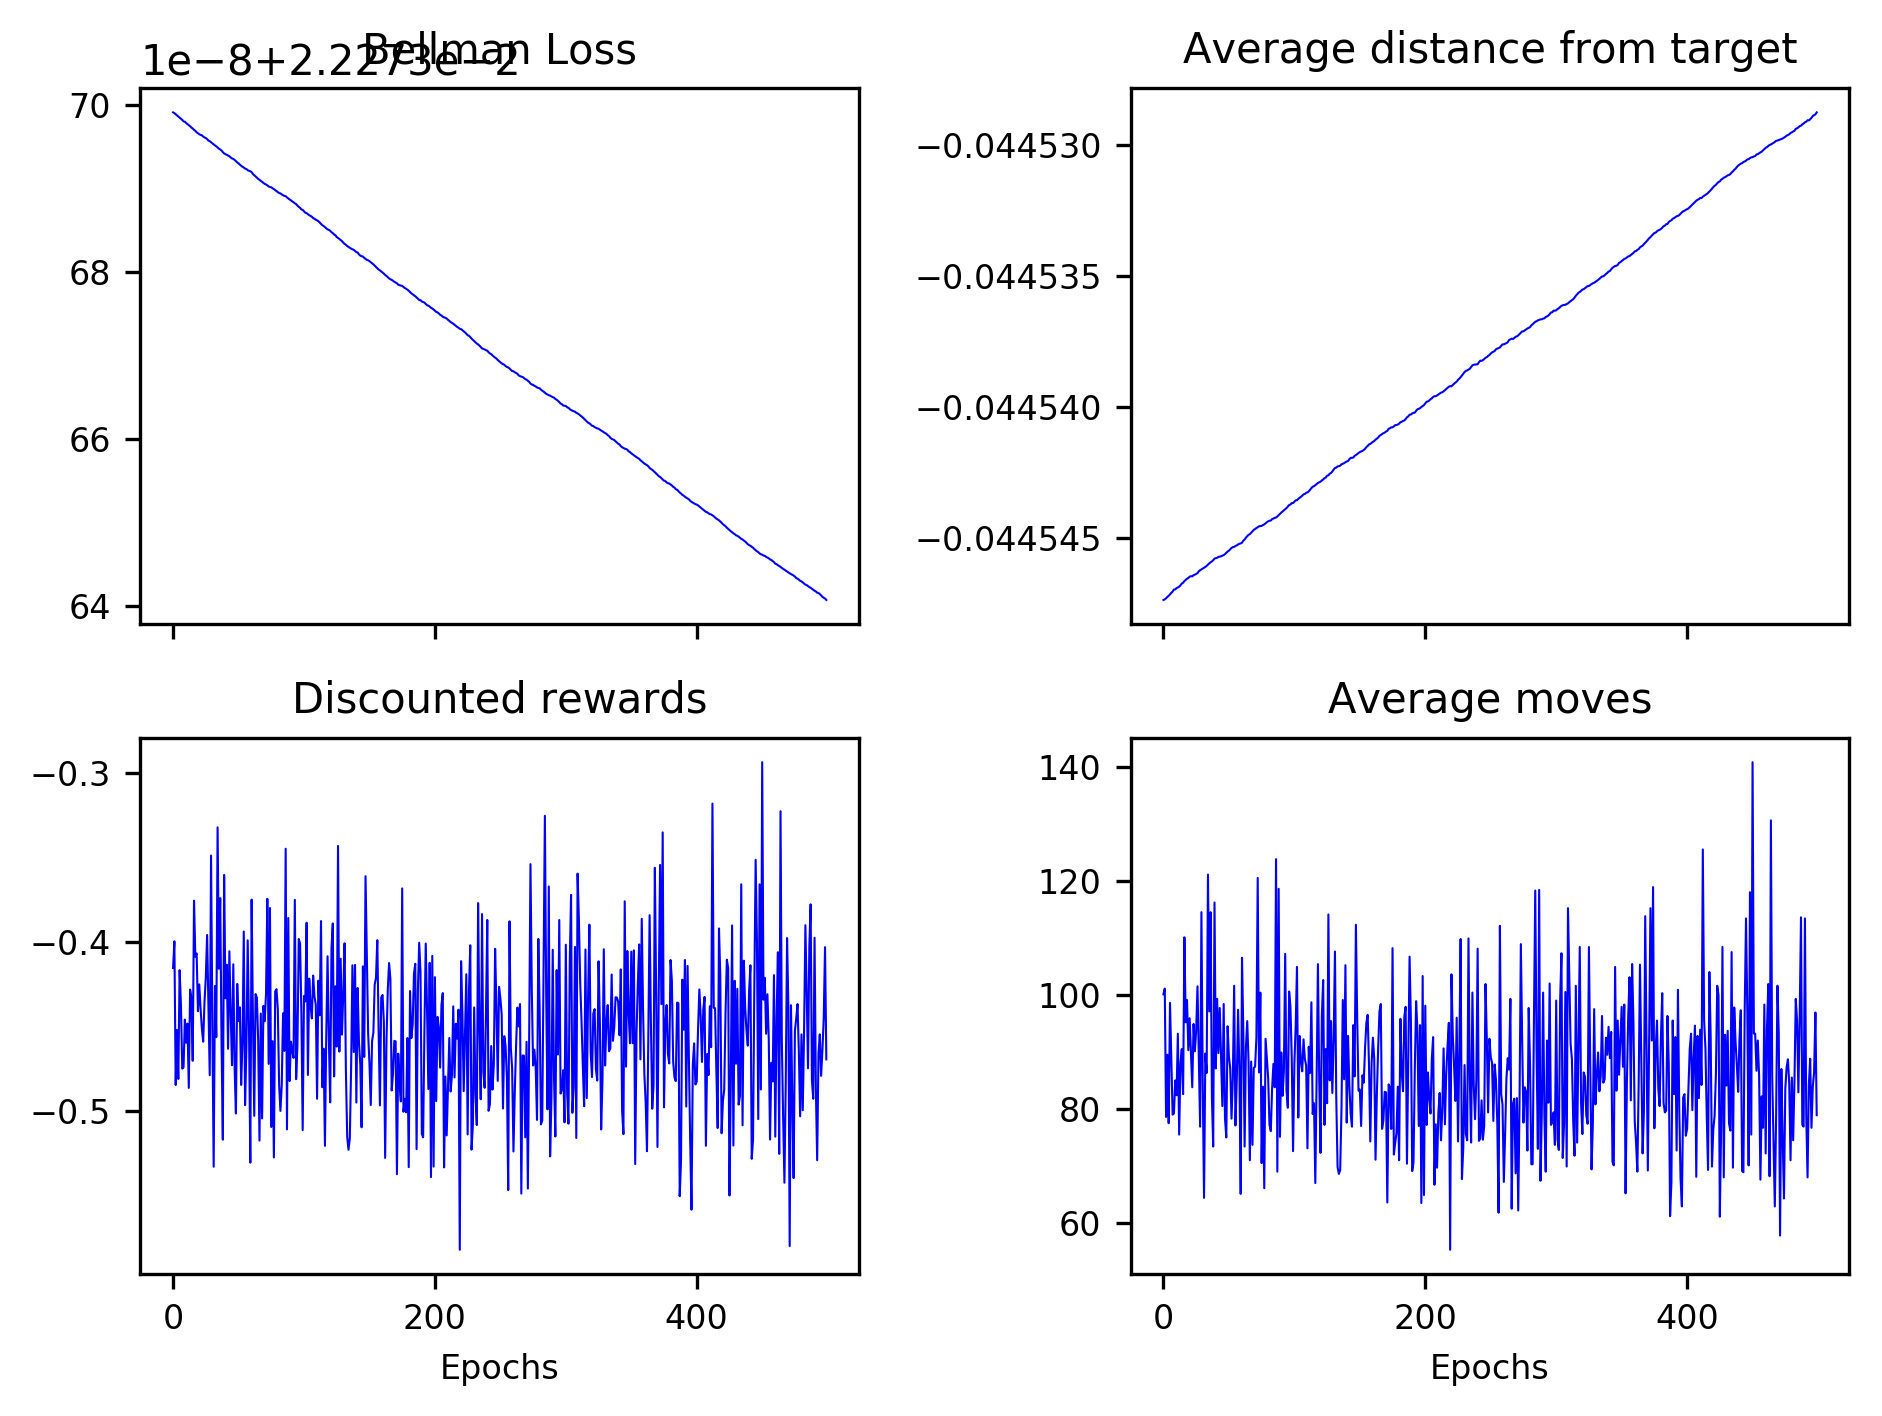
\includegraphics[height=8cm]{{figures/a3a_0.00001}.png}
	\end{center}
    \caption{%
		Batch Q-learning with a linear transform $x \cdot W$. Learning rate = 0.00001.
     }%
\end{figure}

\begin{figure}[H]
    \caption{%
		Batch Q-learning with a linear transform $x \cdot W$. Learning rate = 0.0001.
     }%
	\begin{center}
     	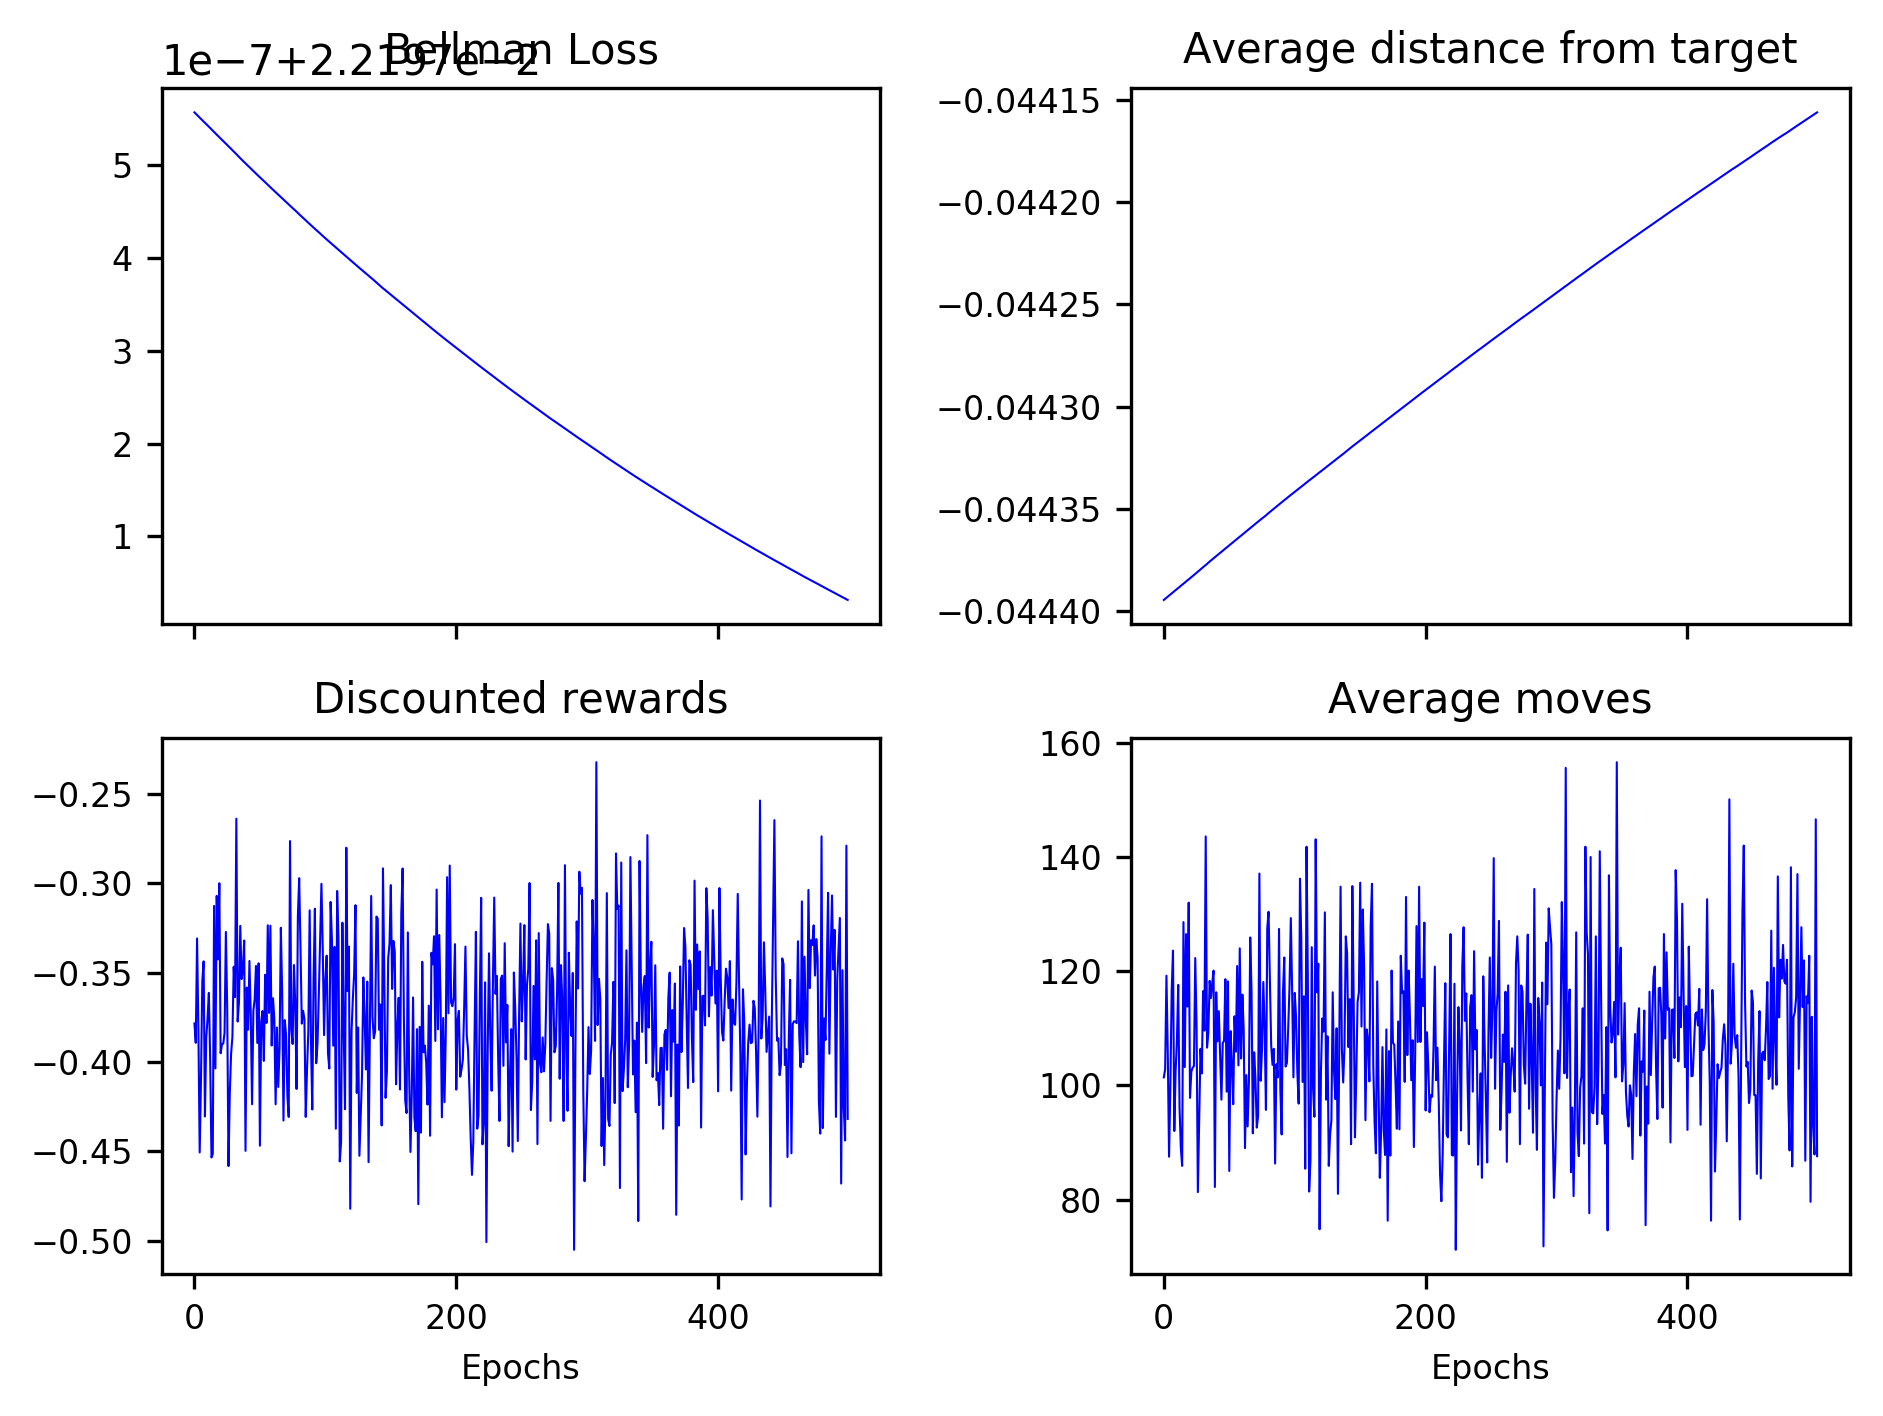
\includegraphics[height=8cm]{{figures/a3a_0.0001}.png}
	\end{center}
\end{figure}

\begin{figure}[H]
	\begin{center}
     	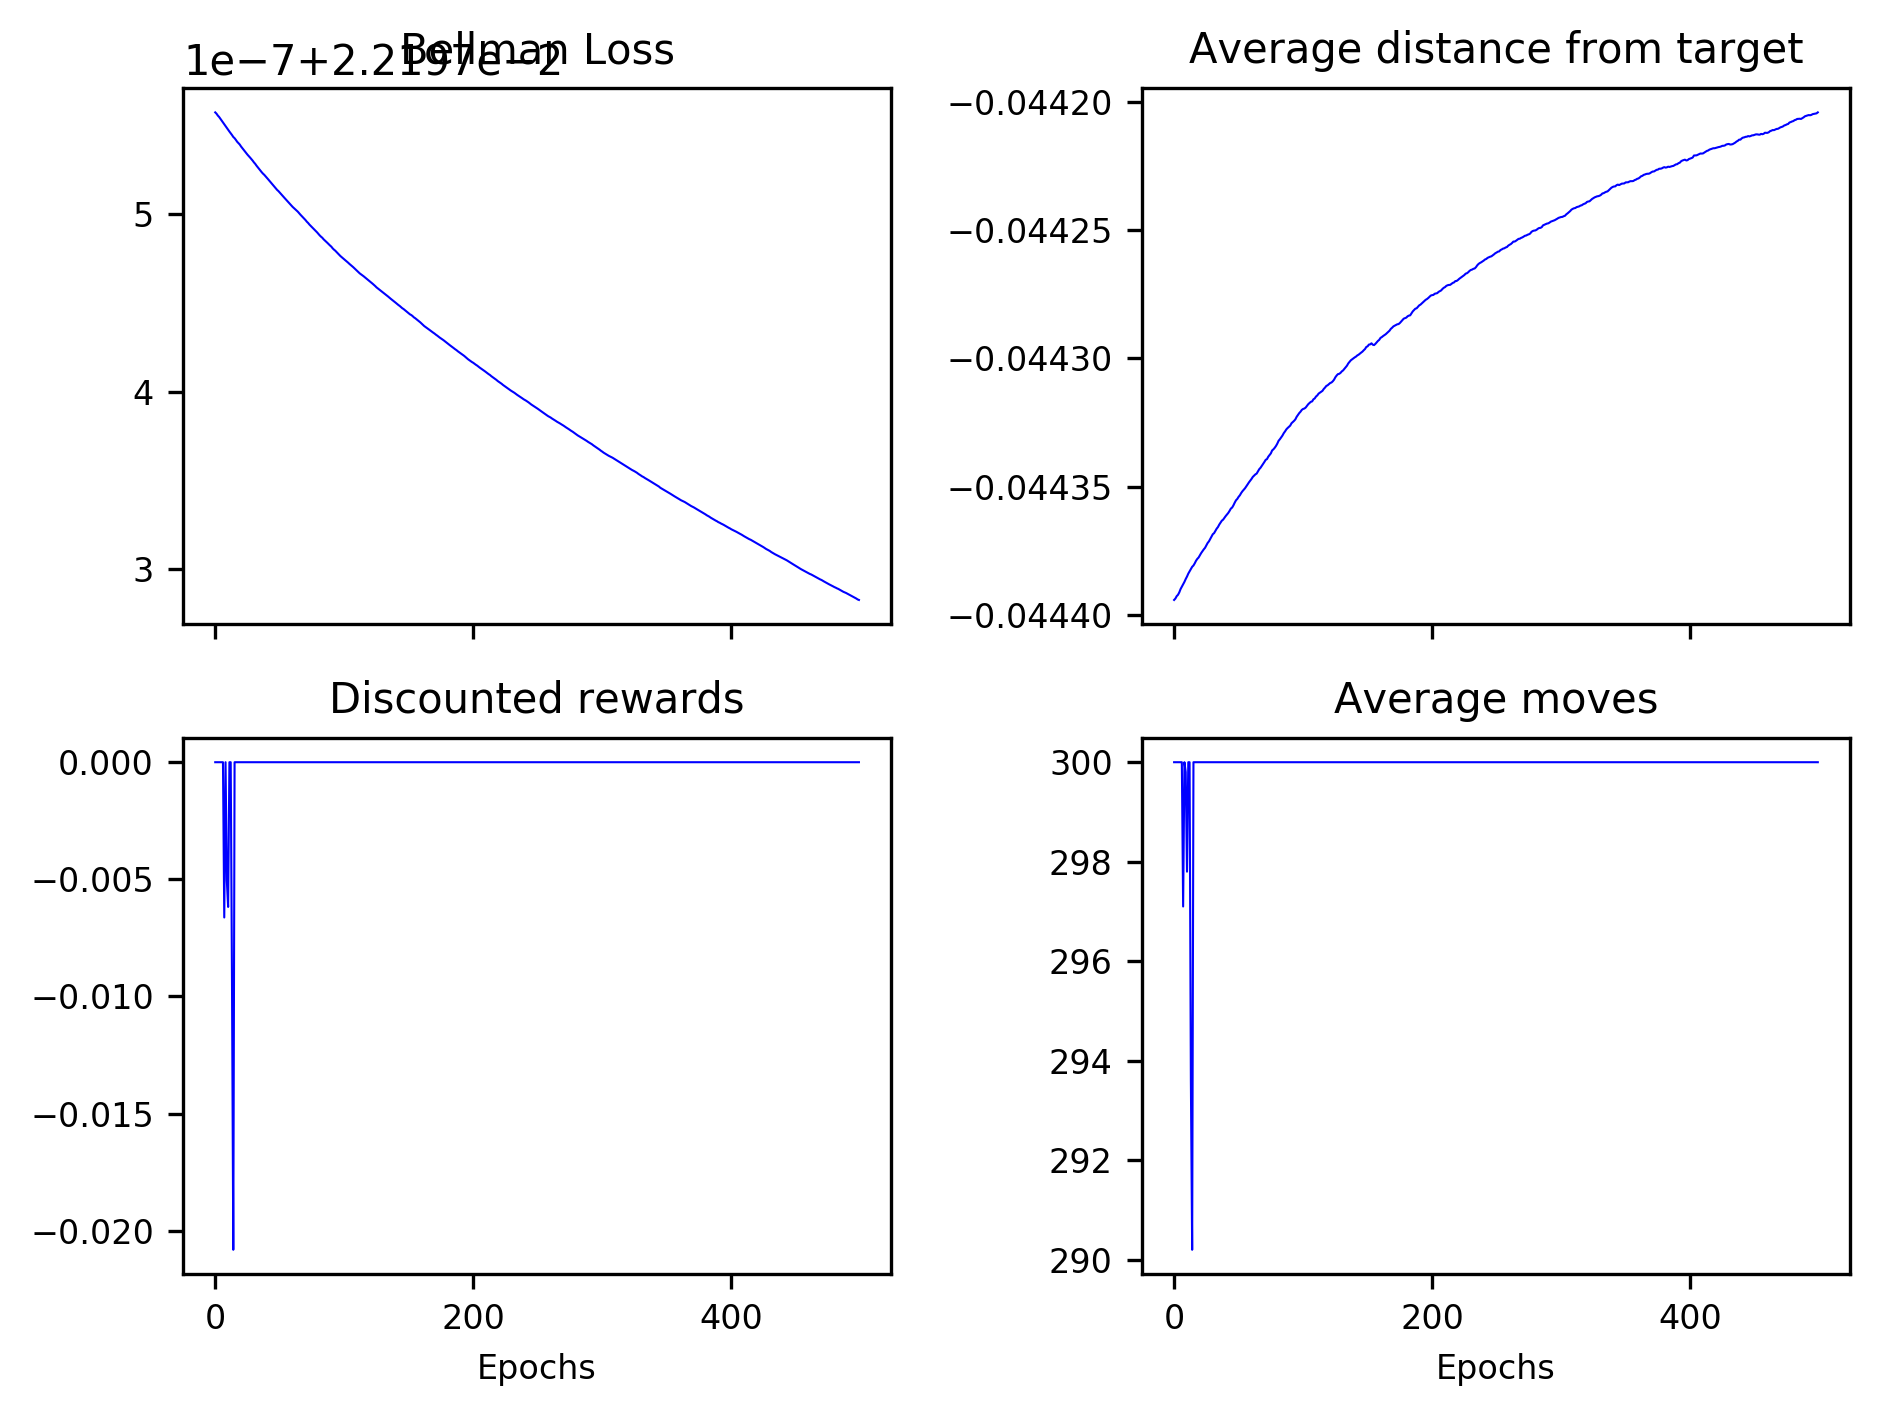
\includegraphics[height=8cm]{{figures/a3a_0.001}.png}
	\end{center}
    \caption{%
		Batch Q-learning with a linear transform $x \cdot W$. Learning rate = 0.001.
     }%
\end{figure}

\begin{figure}[H]
    \caption{%
		Batch Q-learning with a linear transform $x \cdot W$. Learning rate = 0.01.
     }%
	\begin{center}
     	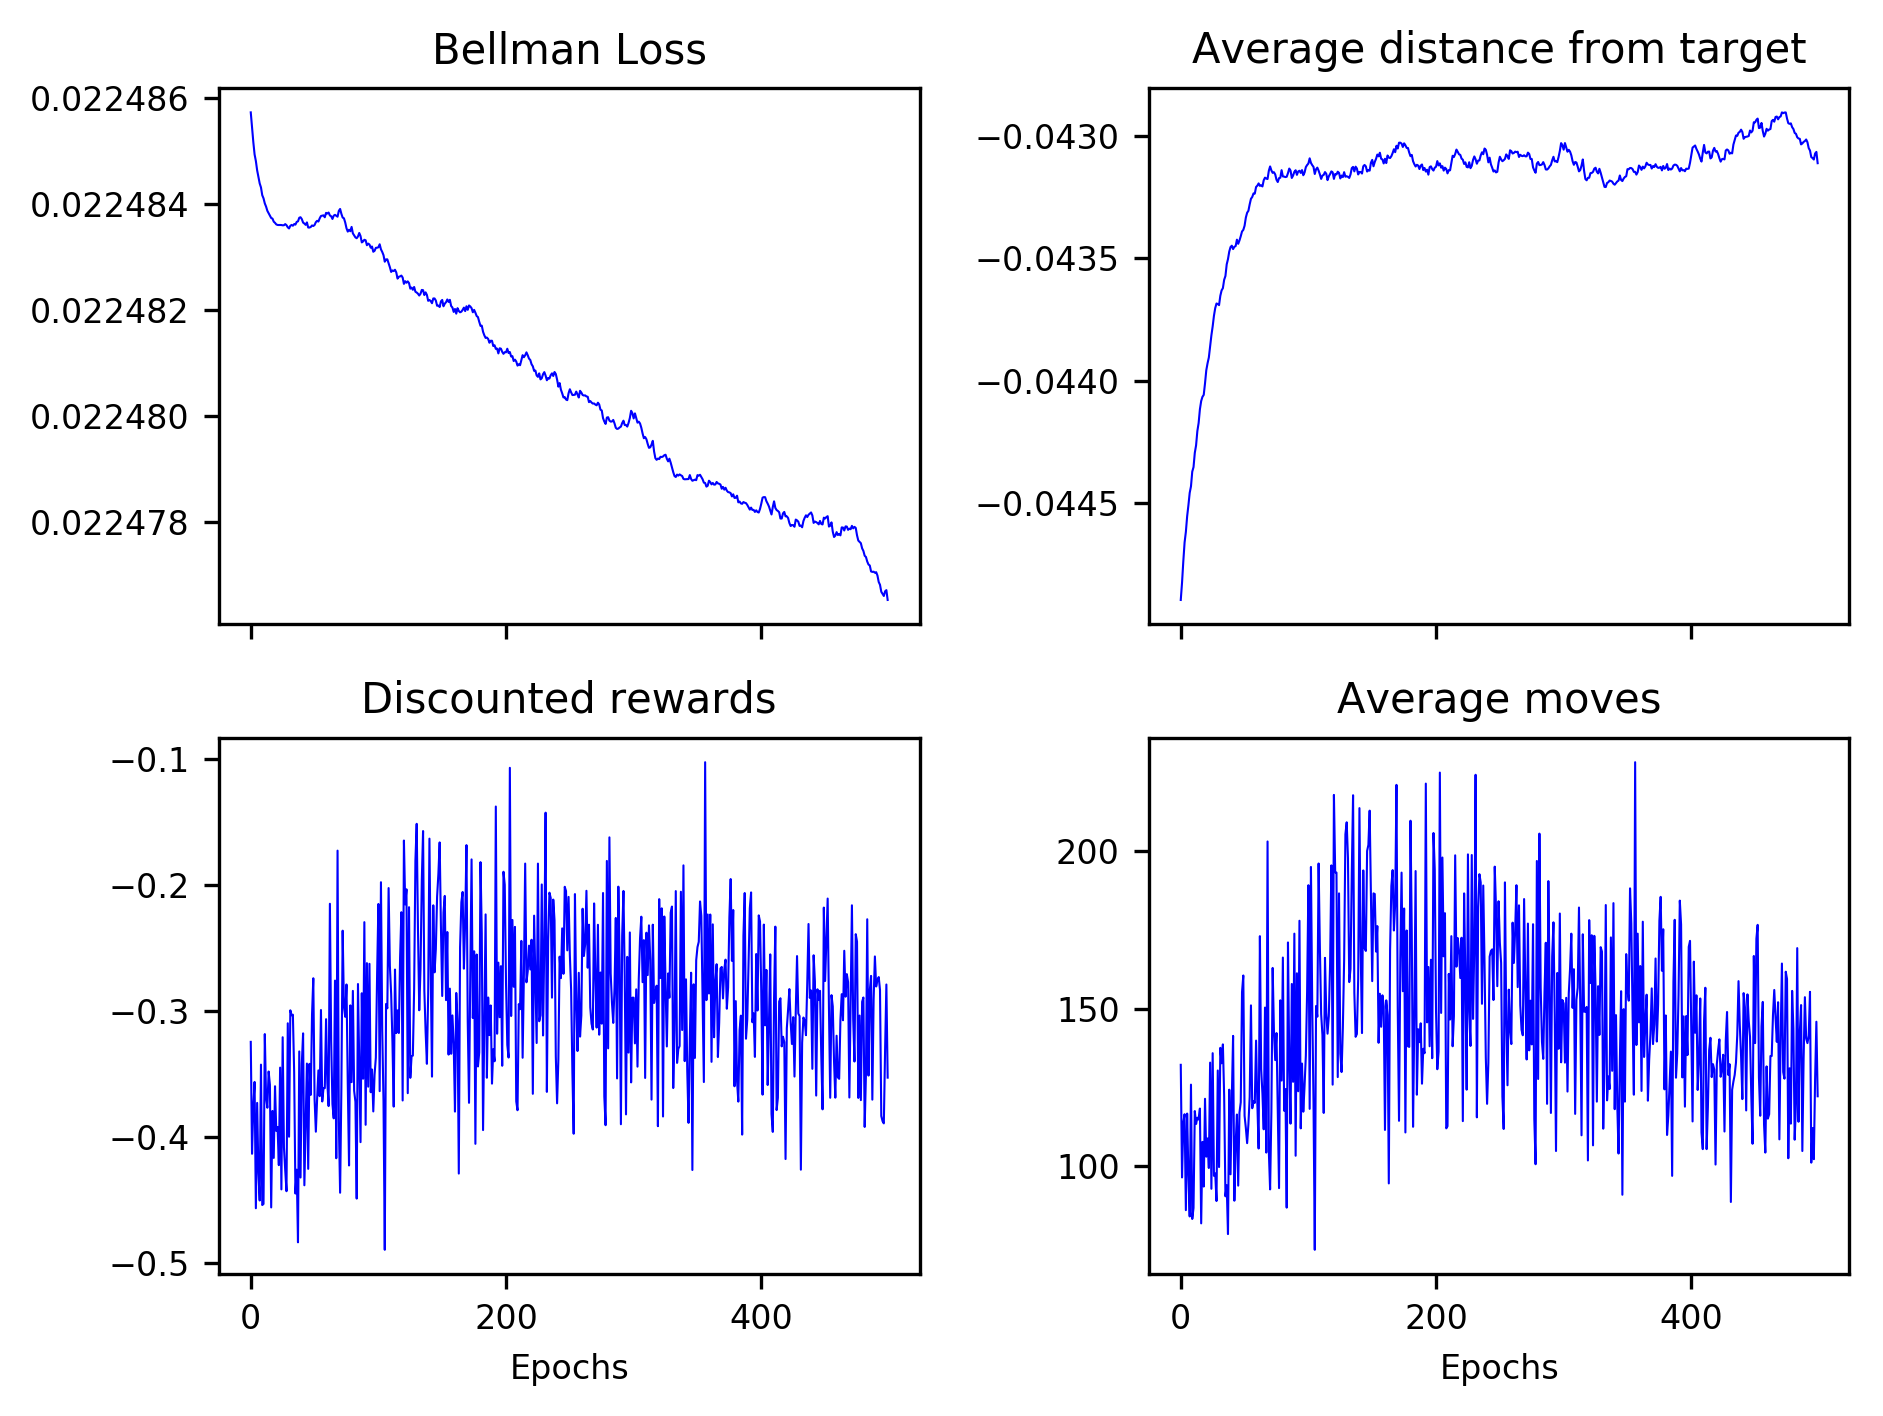
\includegraphics[height=8cm]{{figures/a3a_0.01}.png}
	\end{center}
\end{figure}

\begin{figure}[H]
	\begin{center}
     	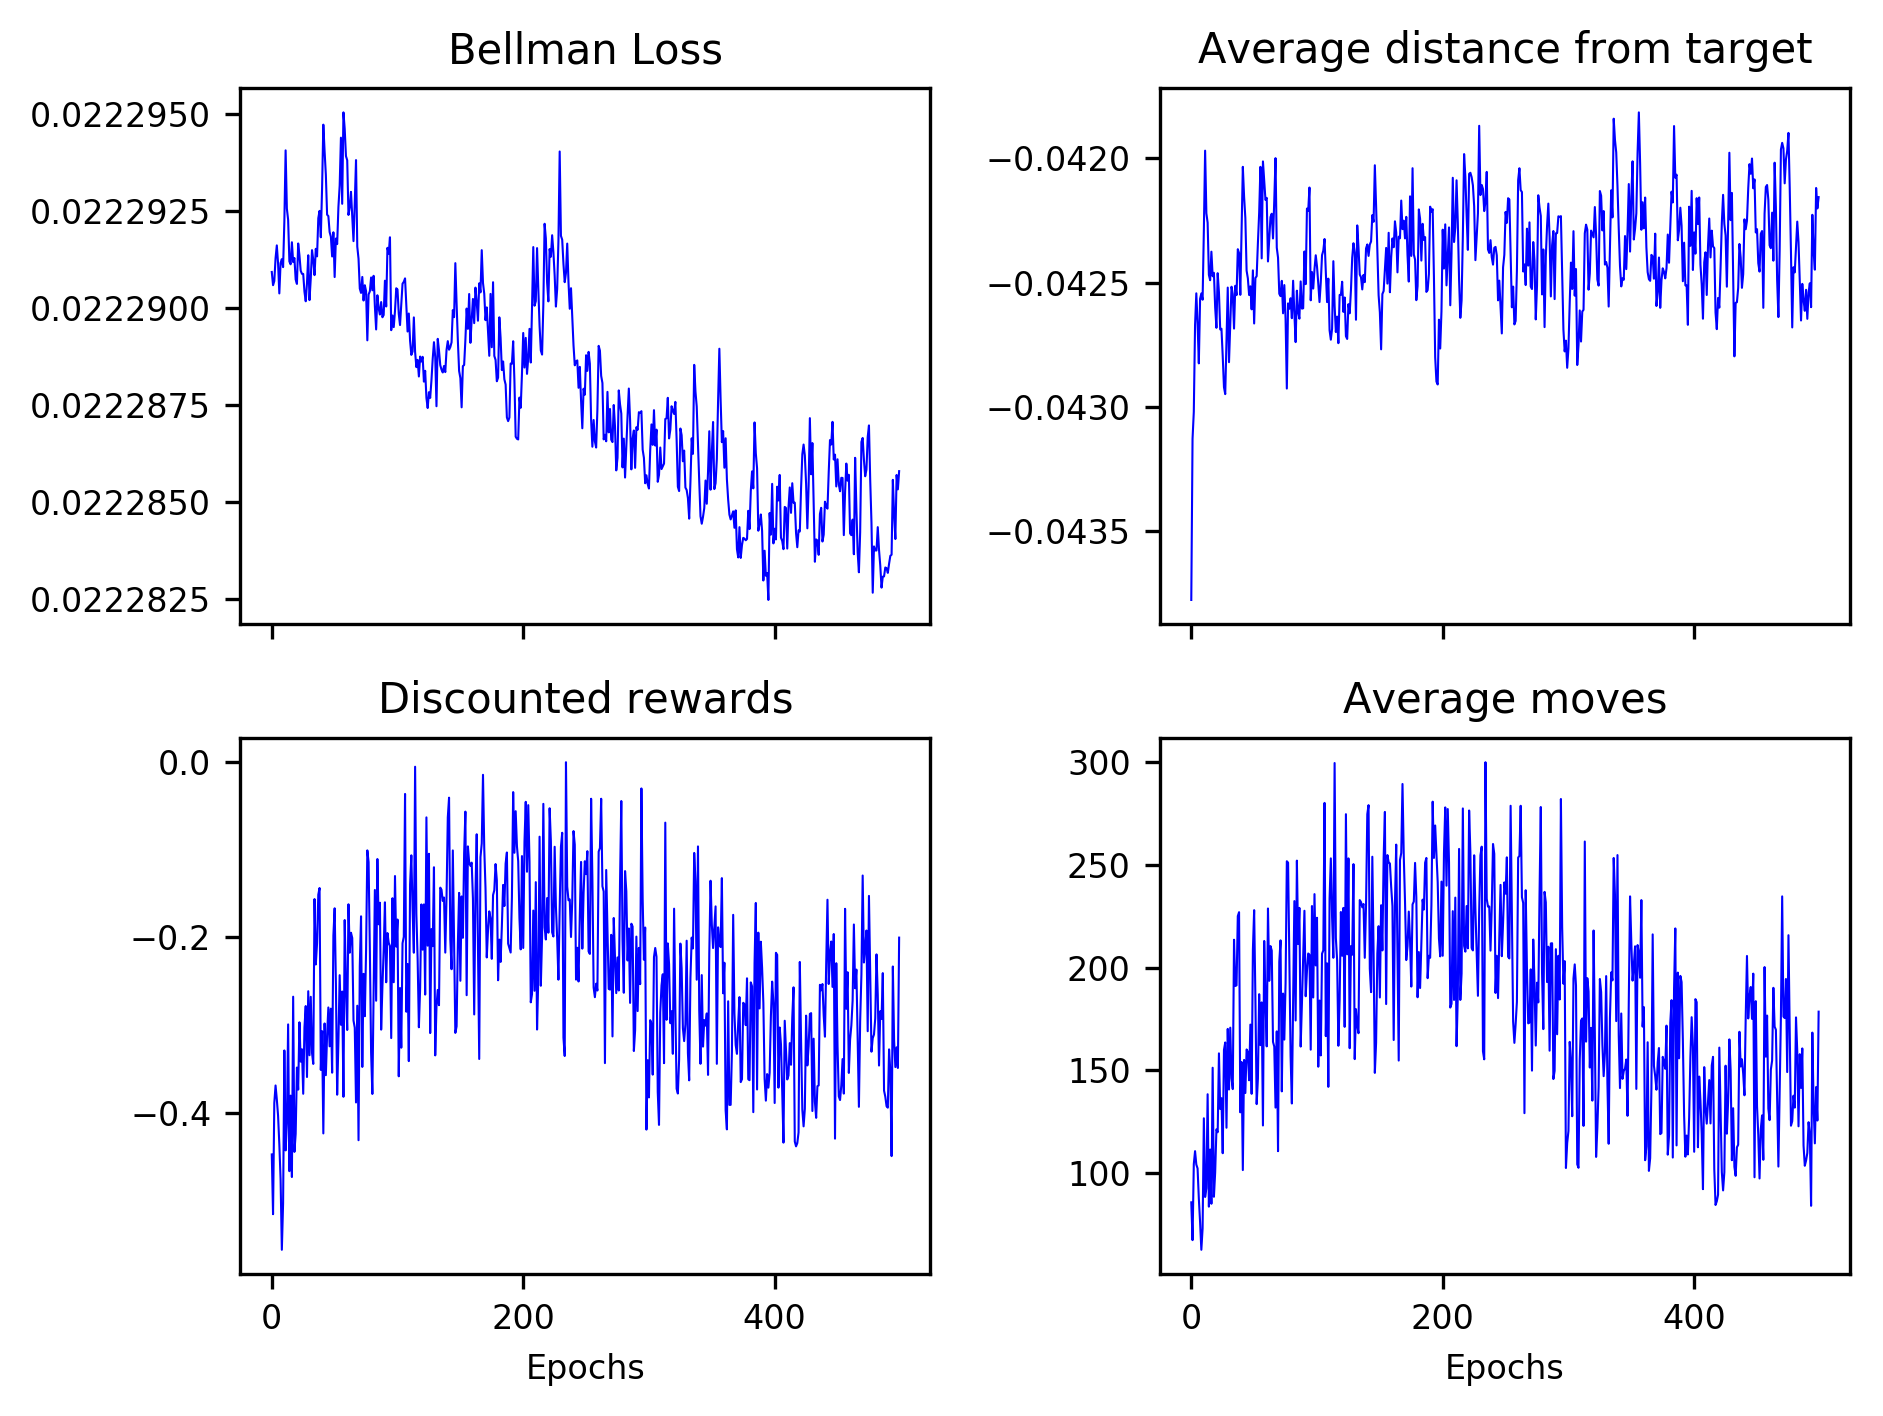
\includegraphics[height=8cm]{{figures/a3a_0.1}.png}
	\end{center}
    \caption{%
		Batch Q-learning with a linear transform $x \cdot W$. Learning rate = 0.1.
     }%
\end{figure}

\begin{figure}[H]
    \caption{%
		Batch Q-learning with a linear transform $x \cdot W$. Learning rate = 0.5.
     }%
	\begin{center}
     	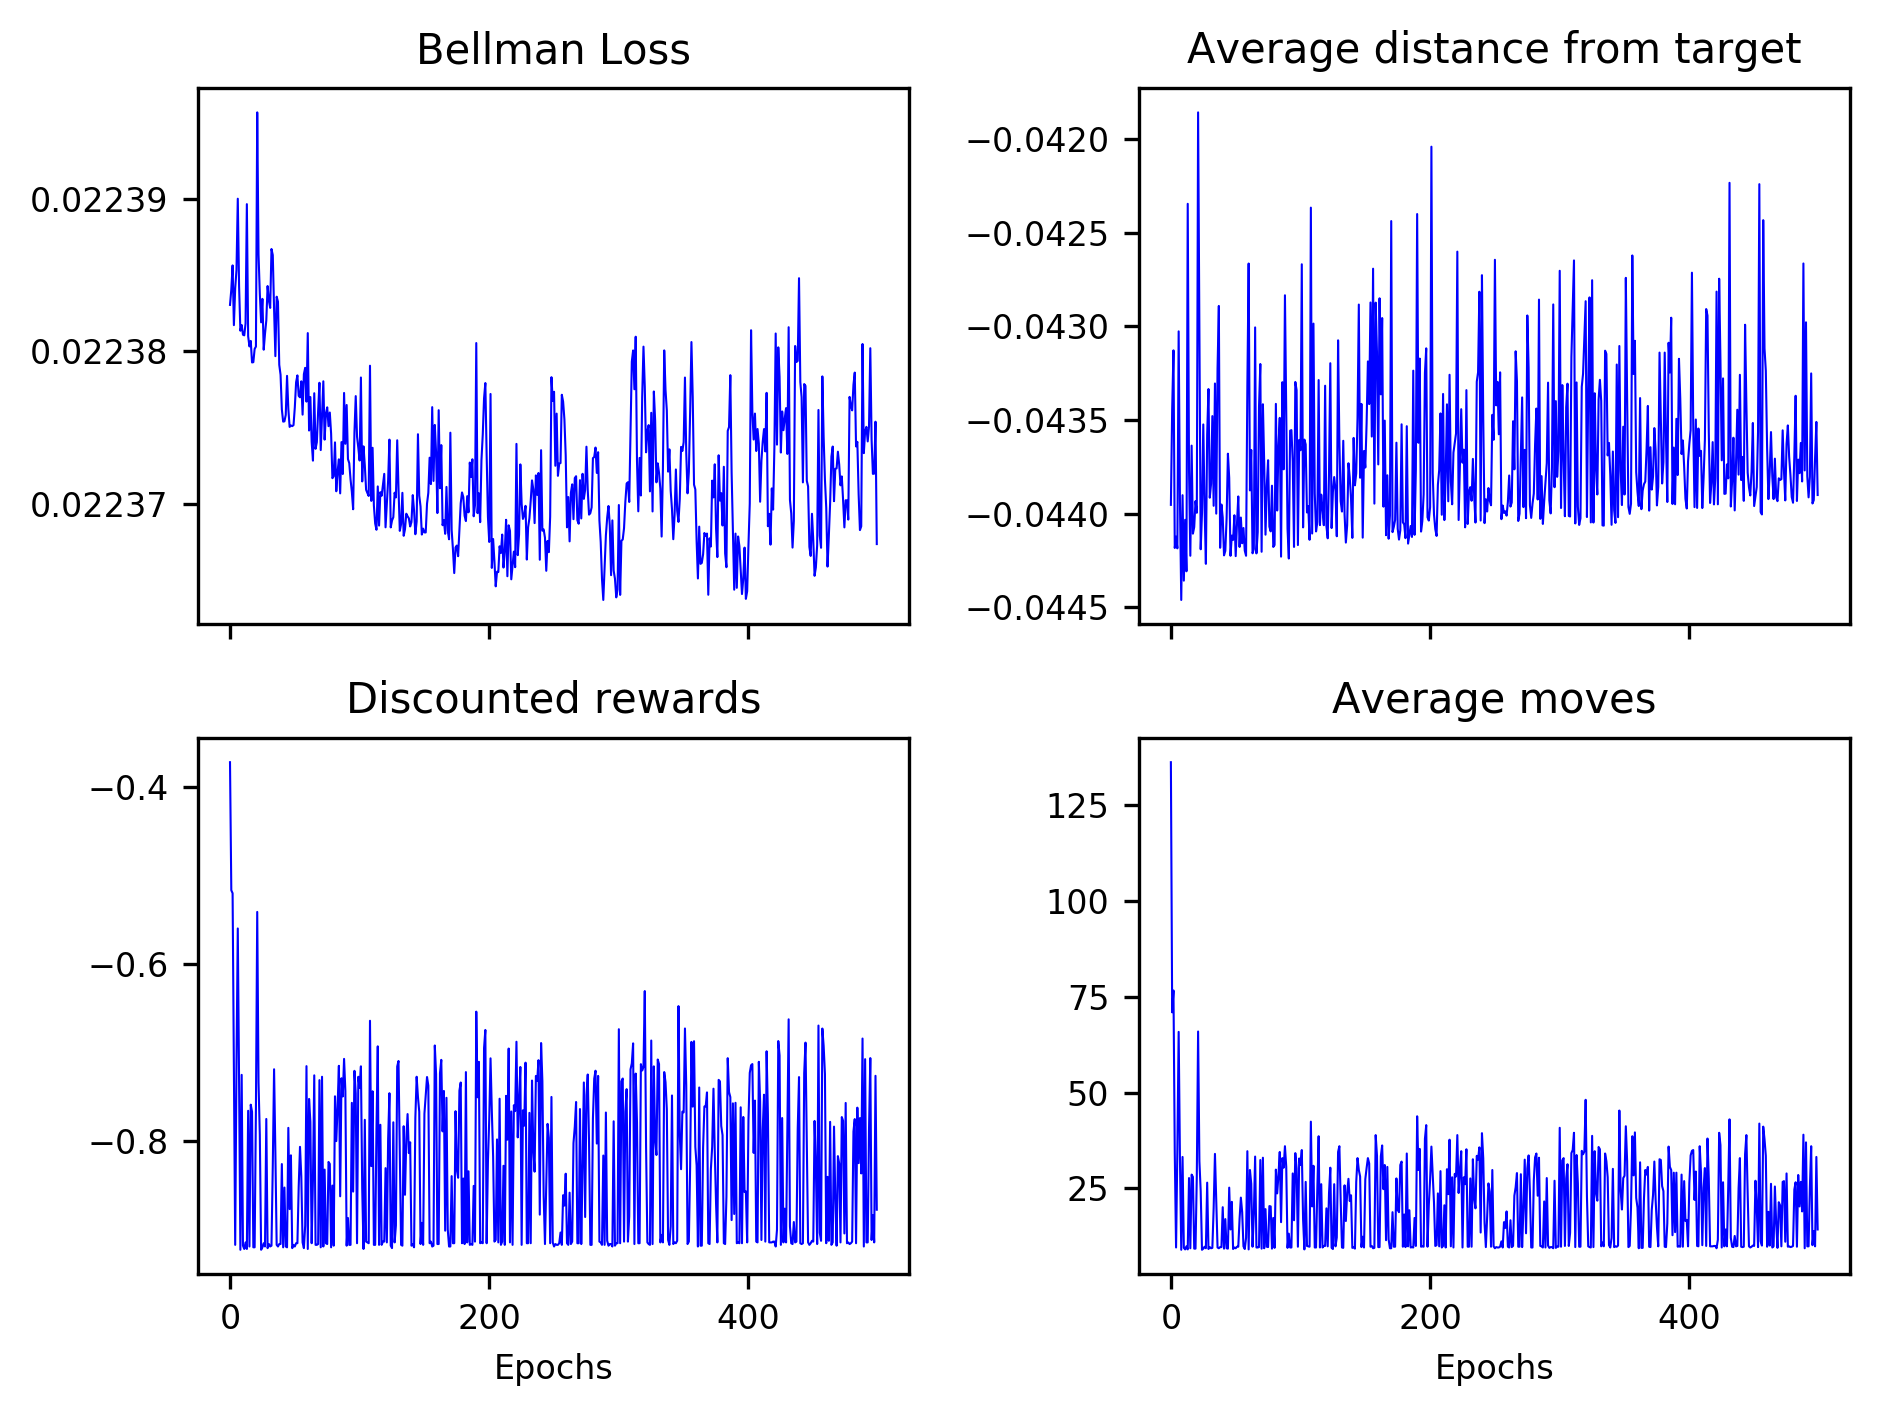
\includegraphics[height=8cm]{{figures/a3a_0.5}.png}
	\end{center}
\end{figure}


\subsubsection{Hidden layer with 100 units, followed by ReLU}

The single-layer neural network did not include any biases. Experimentally, biases proved to be much harder to train, and so were dropped from further experiments. All further experiments in part A do not have biases. Evaluation was over 10 episodes after every epoch of training.

% a3b

\begin{figure}[H]
    \caption{%
		Batch Q-learning with neural network with one hidden layer of 100 units. Learning rate = 0.00001.
     }%
	\begin{center}
     	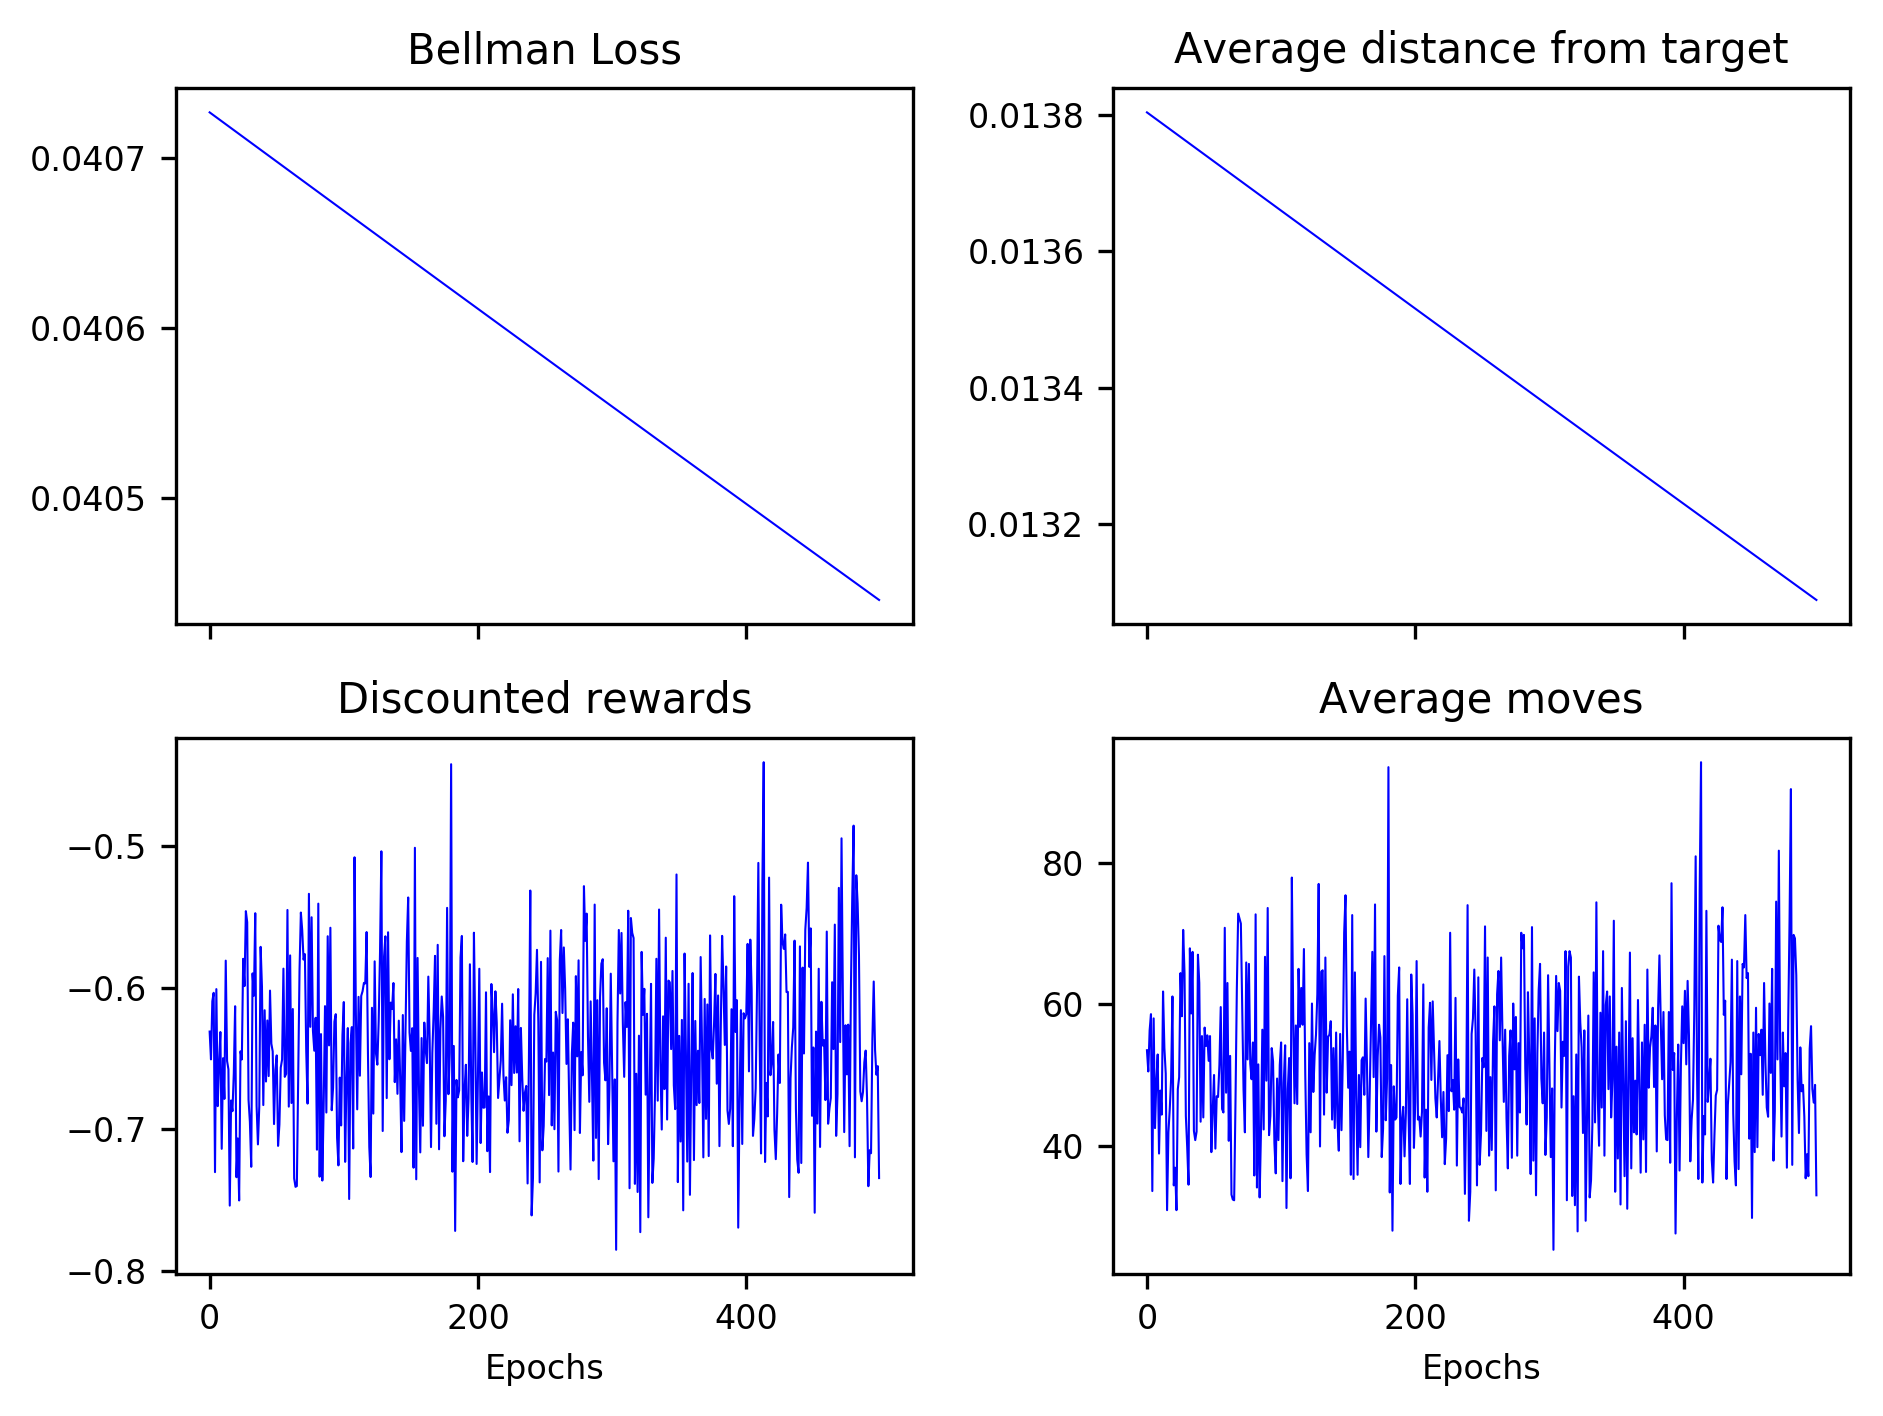
\includegraphics[height=8cm]{{figures/a3b_0.00001}.png}
	\end{center}
\end{figure}

\begin{figure}[H]
	\begin{center}
     	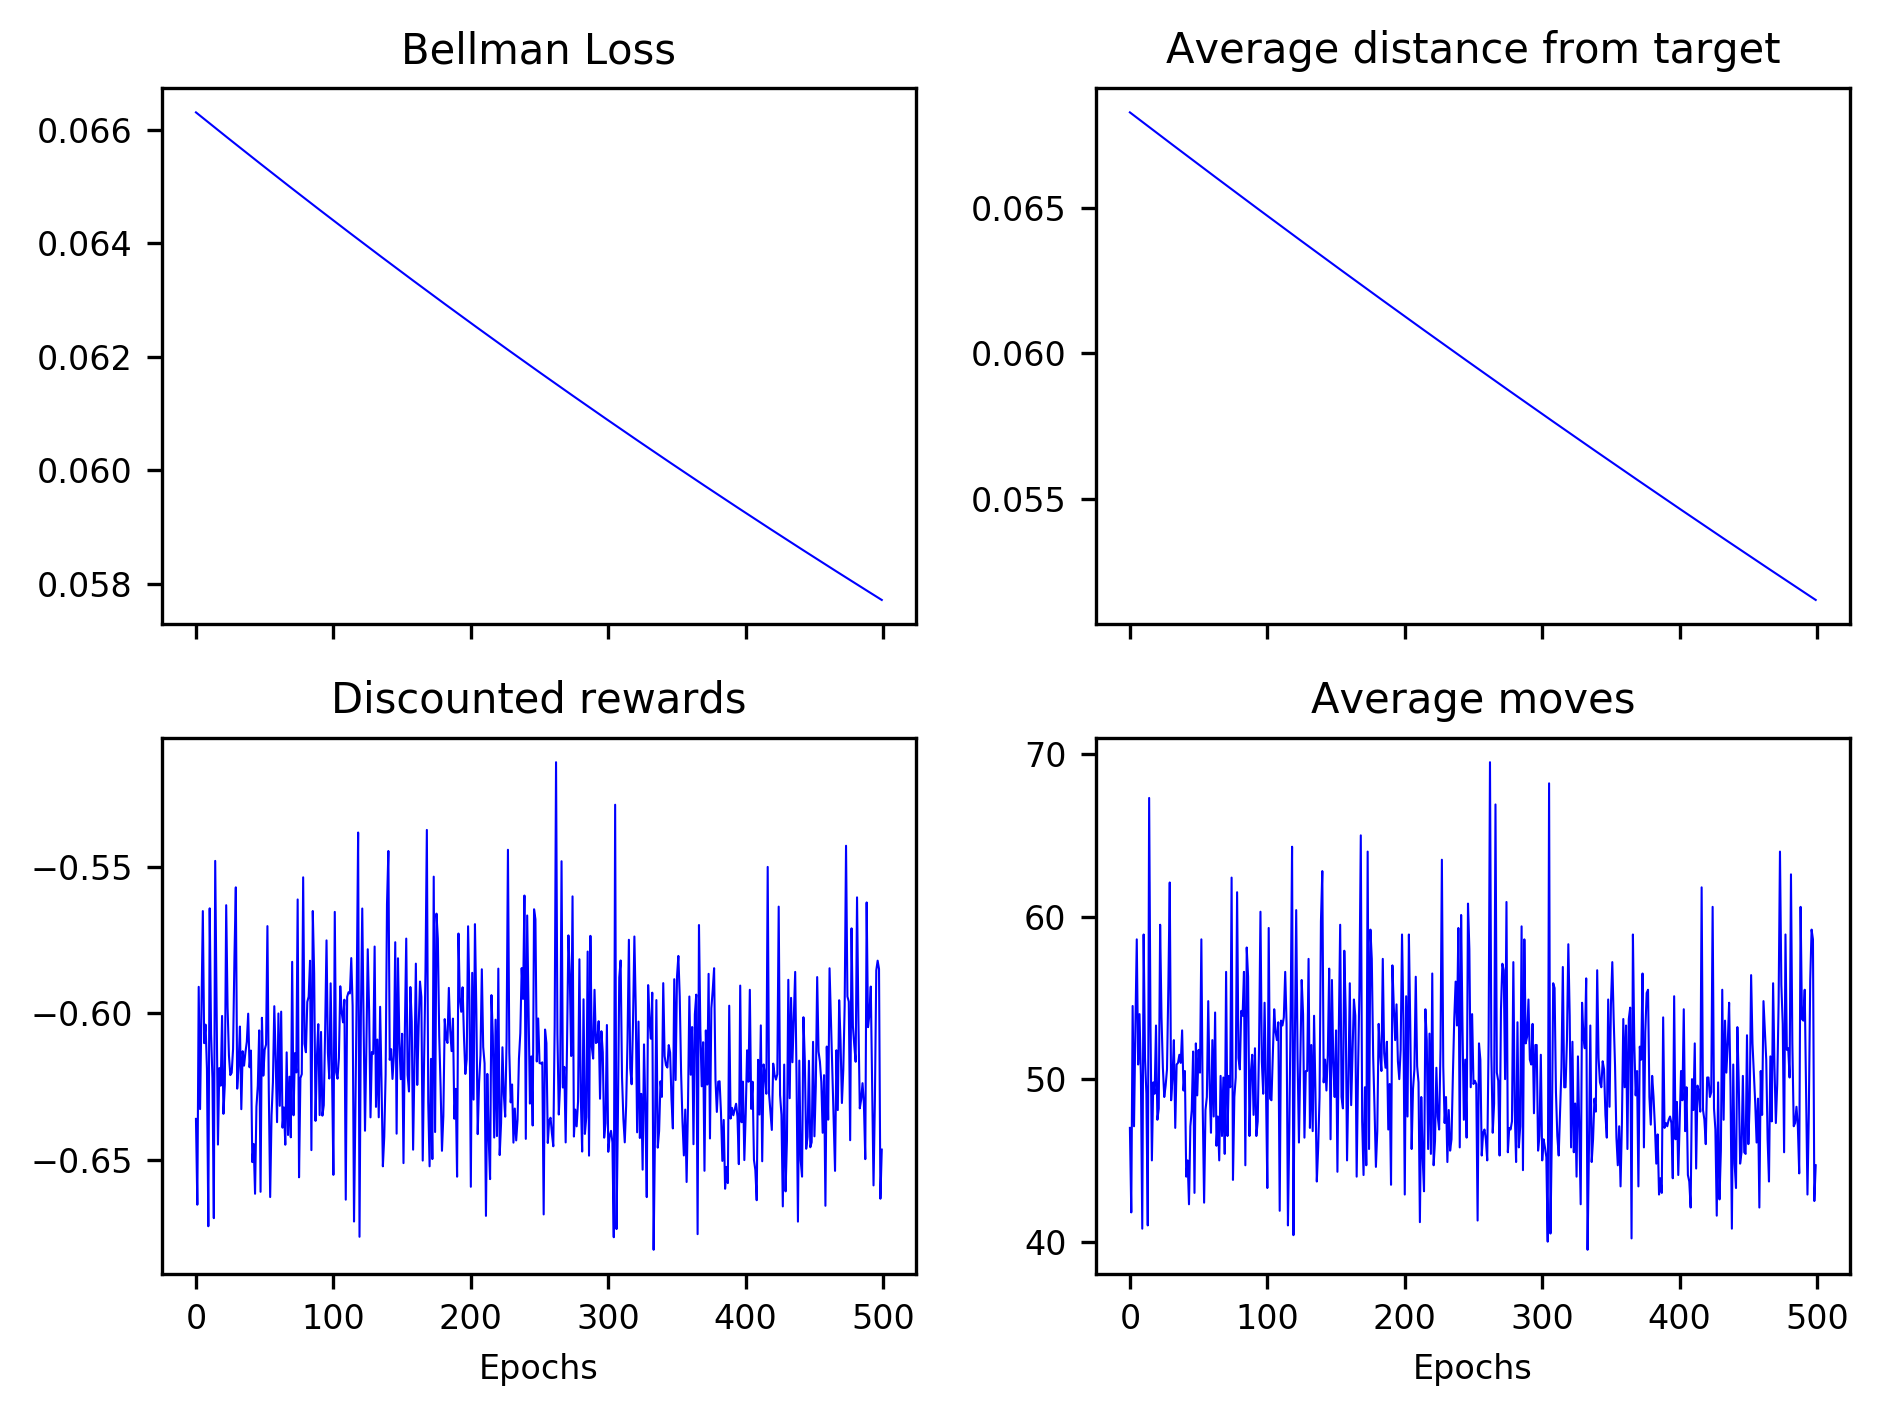
\includegraphics[height=8cm]{{figures/a3b_0.0001}.png}
	\end{center}
    \caption{%
		Batch Q-learning with neural network with one hidden layer of 100 units. Learning rate = 0.0001.
     }%
\end{figure}

\begin{figure}[H]
    \caption{%
		Batch Q-learning with neural network with one hidden layer of 100 units. Learning rate = 0.001.
     }%
	\begin{center}
     	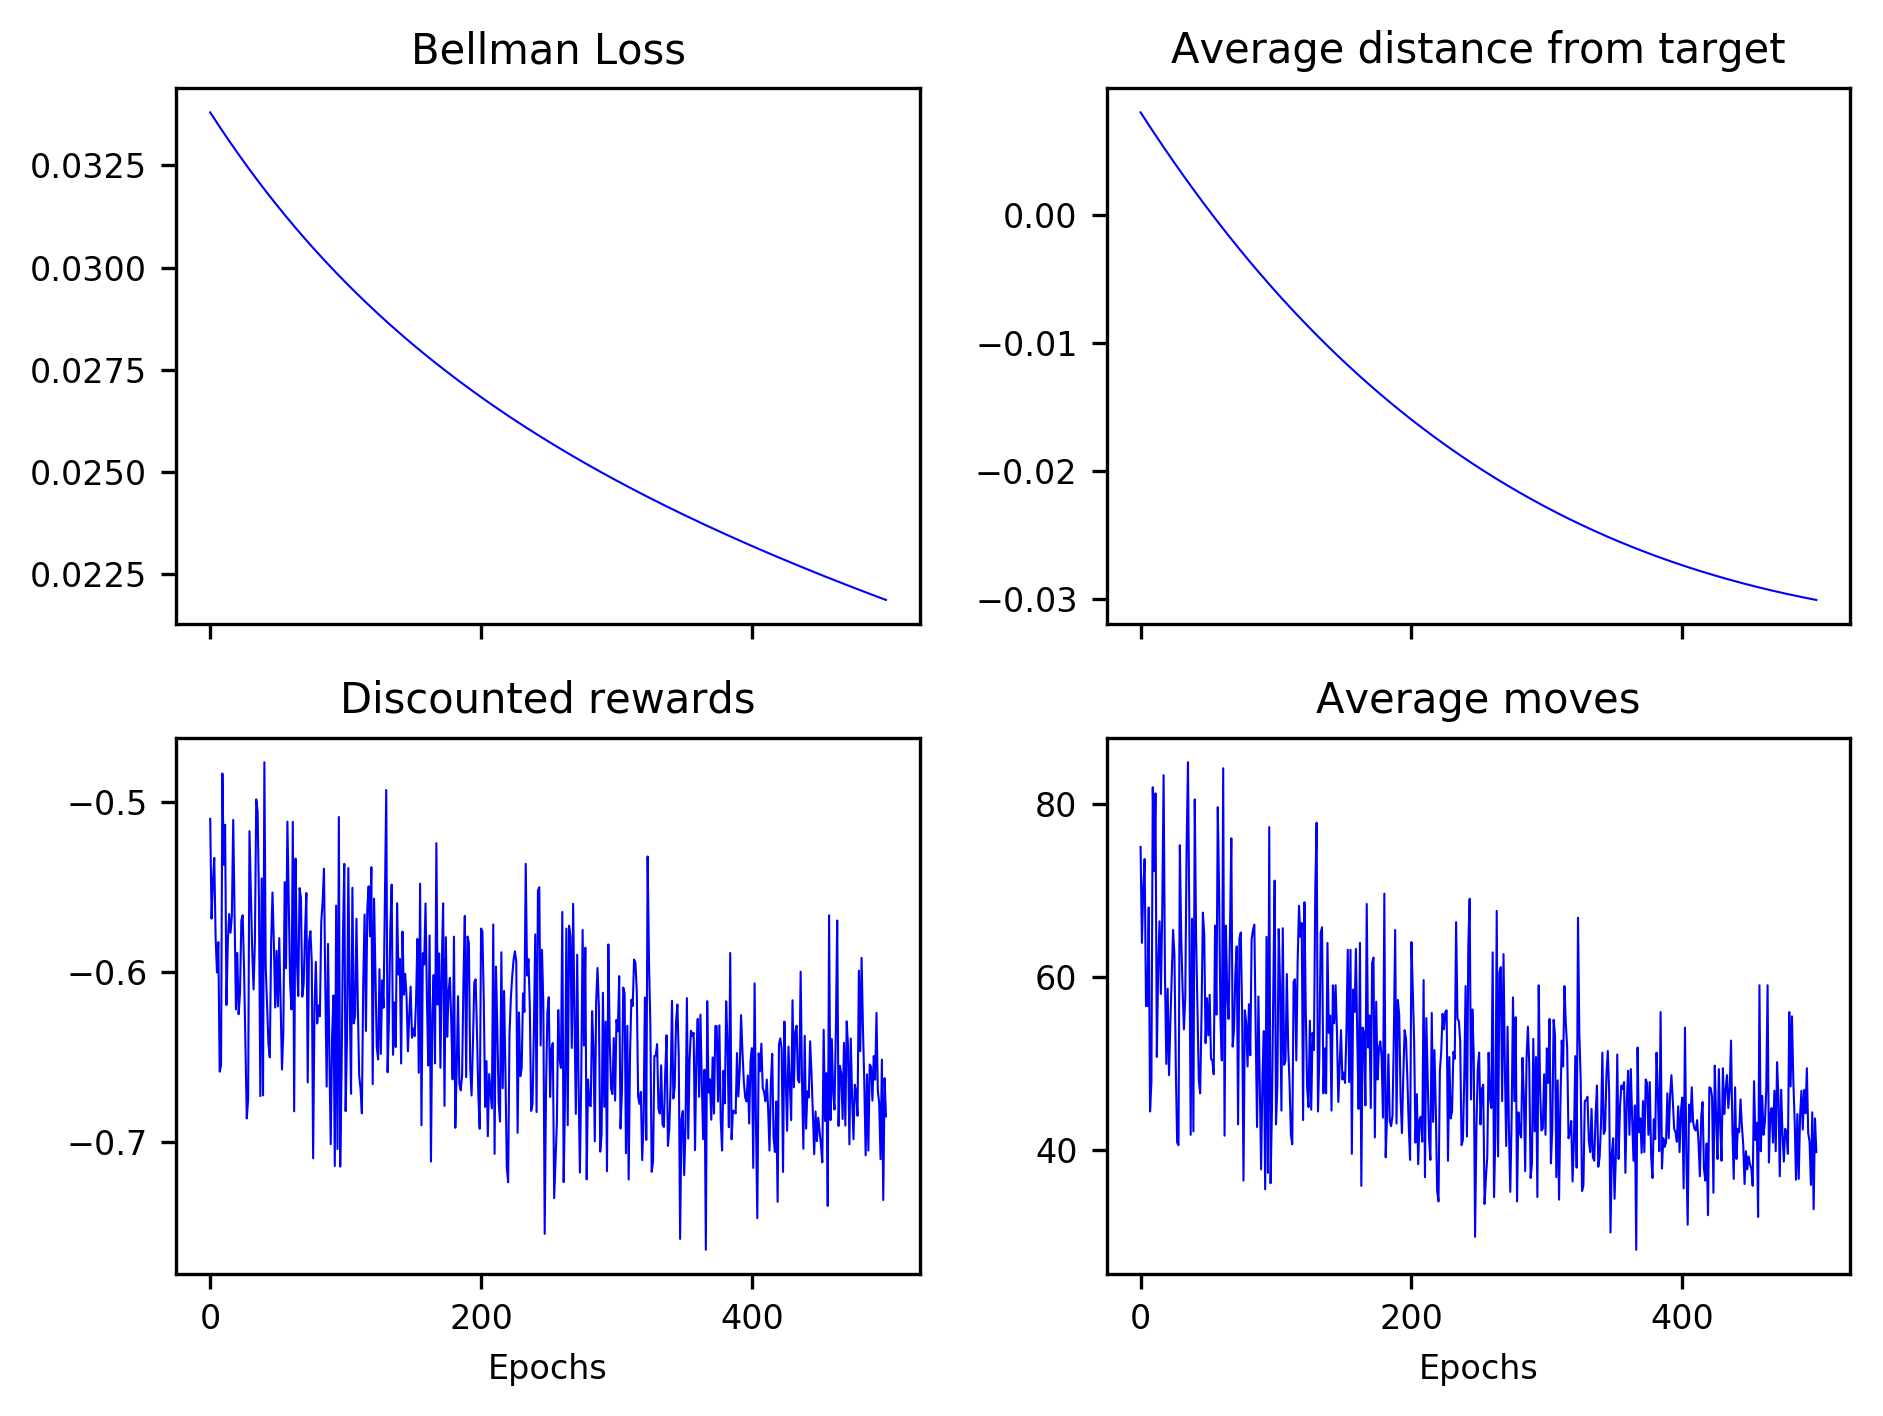
\includegraphics[height=8cm]{{figures/a3b_0.001}.png}
	\end{center}
\end{figure}

\begin{figure}[H]
	\begin{center}
     	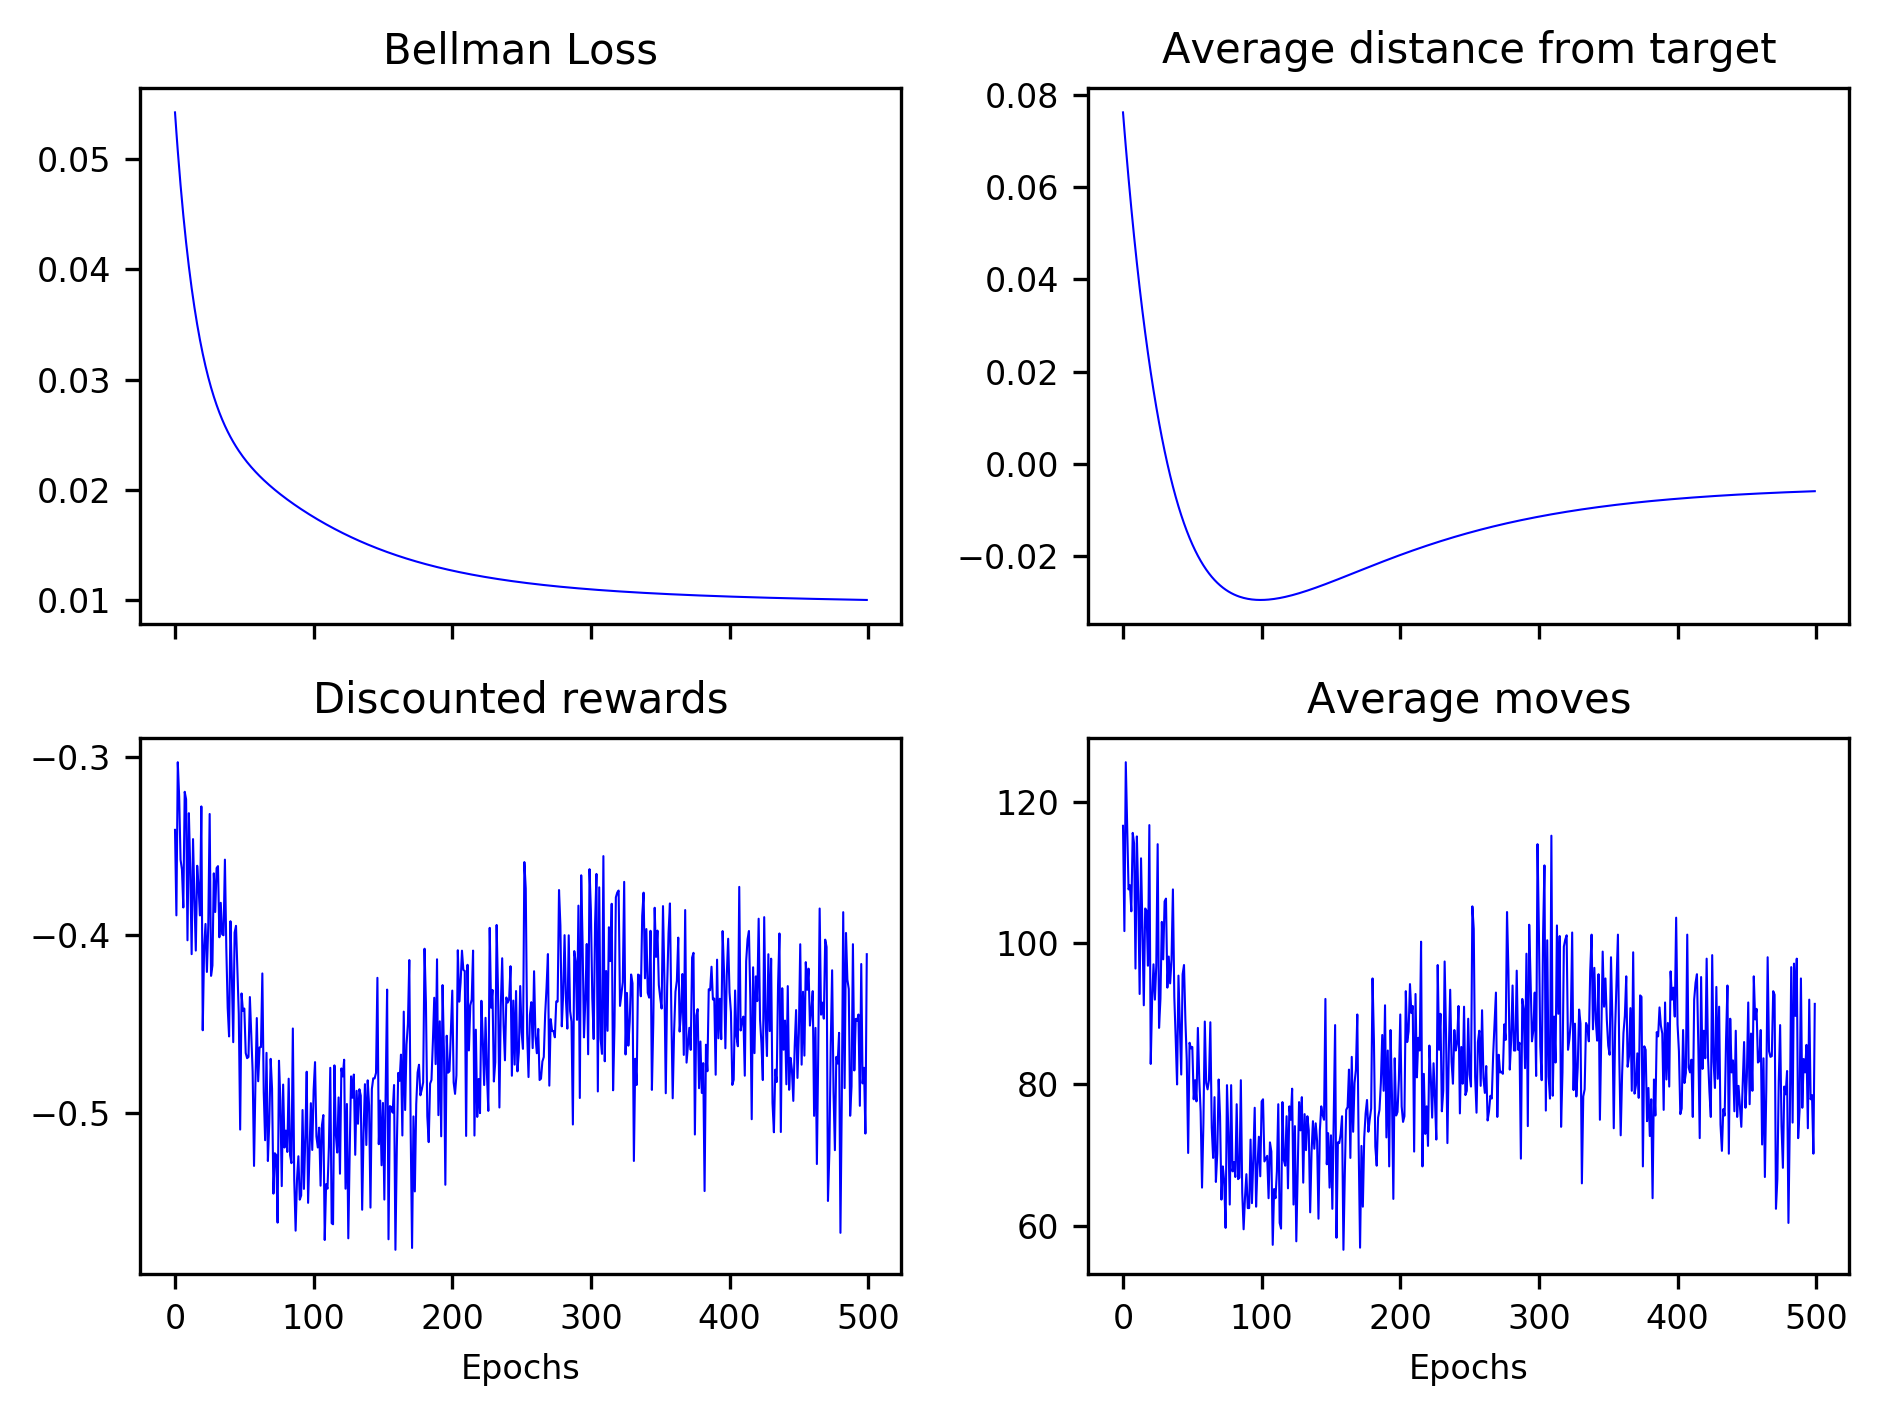
\includegraphics[height=8cm]{{figures/a3b_0.01}.png}
	\end{center}
    \caption{%
		Batch Q-learning with neural network with one hidden layer of 100 units. Learning rate = 0.01.
     }%
\end{figure}

\begin{figure}[H]
    \caption{%
		Batch Q-learning with neural network with one hidden layer of 100 units. Learning rate = 0.1.
     }%
	\begin{center}
     	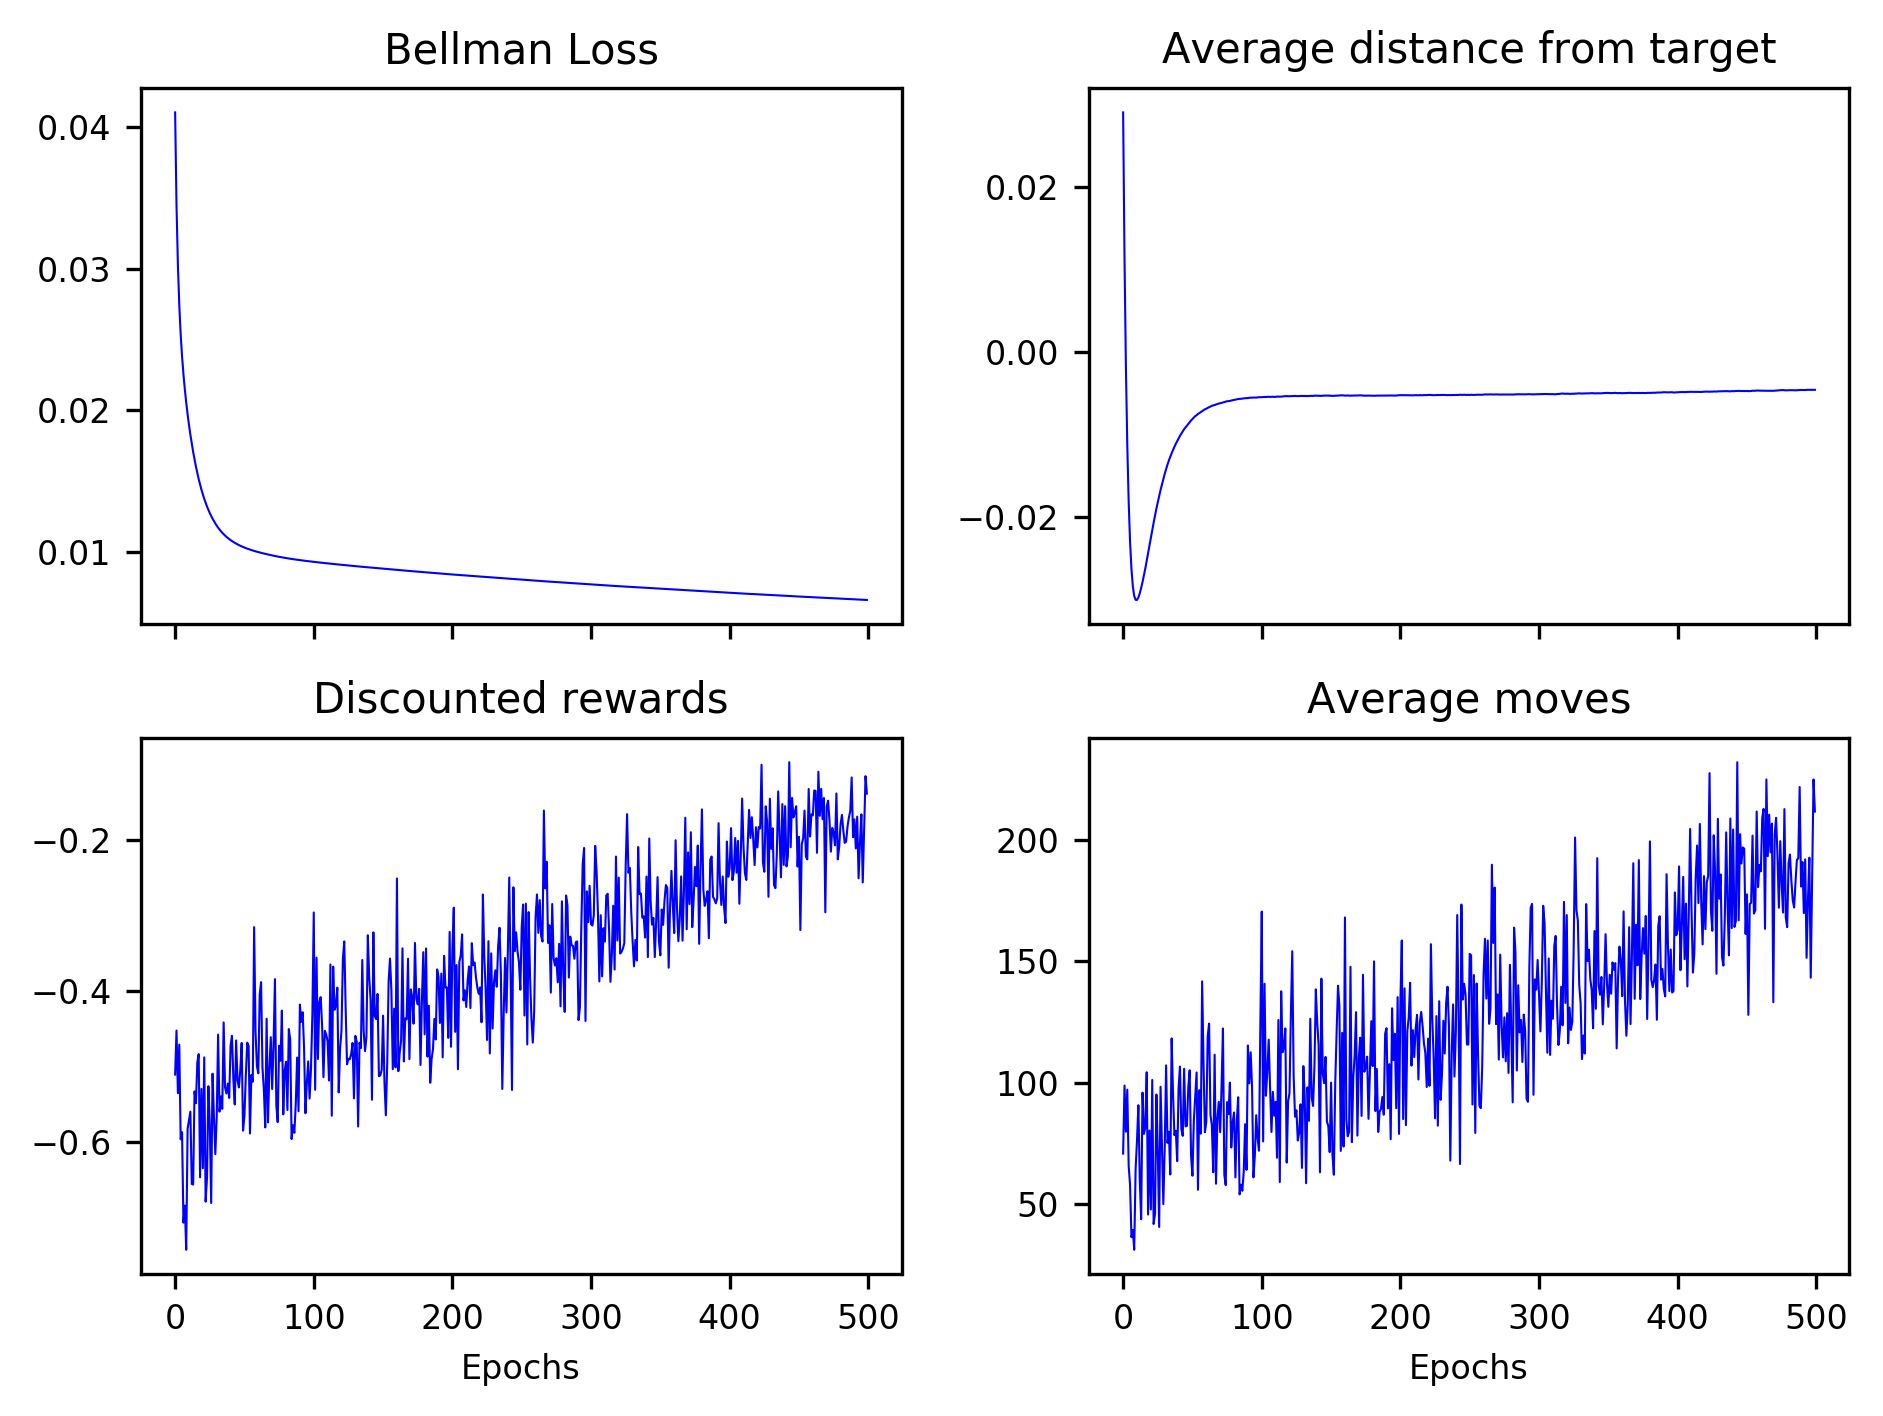
\includegraphics[height=8cm]{{figures/a3b_0.1}.png}
	\end{center}
\end{figure}

\begin{figure}[H]
	\begin{center}
     	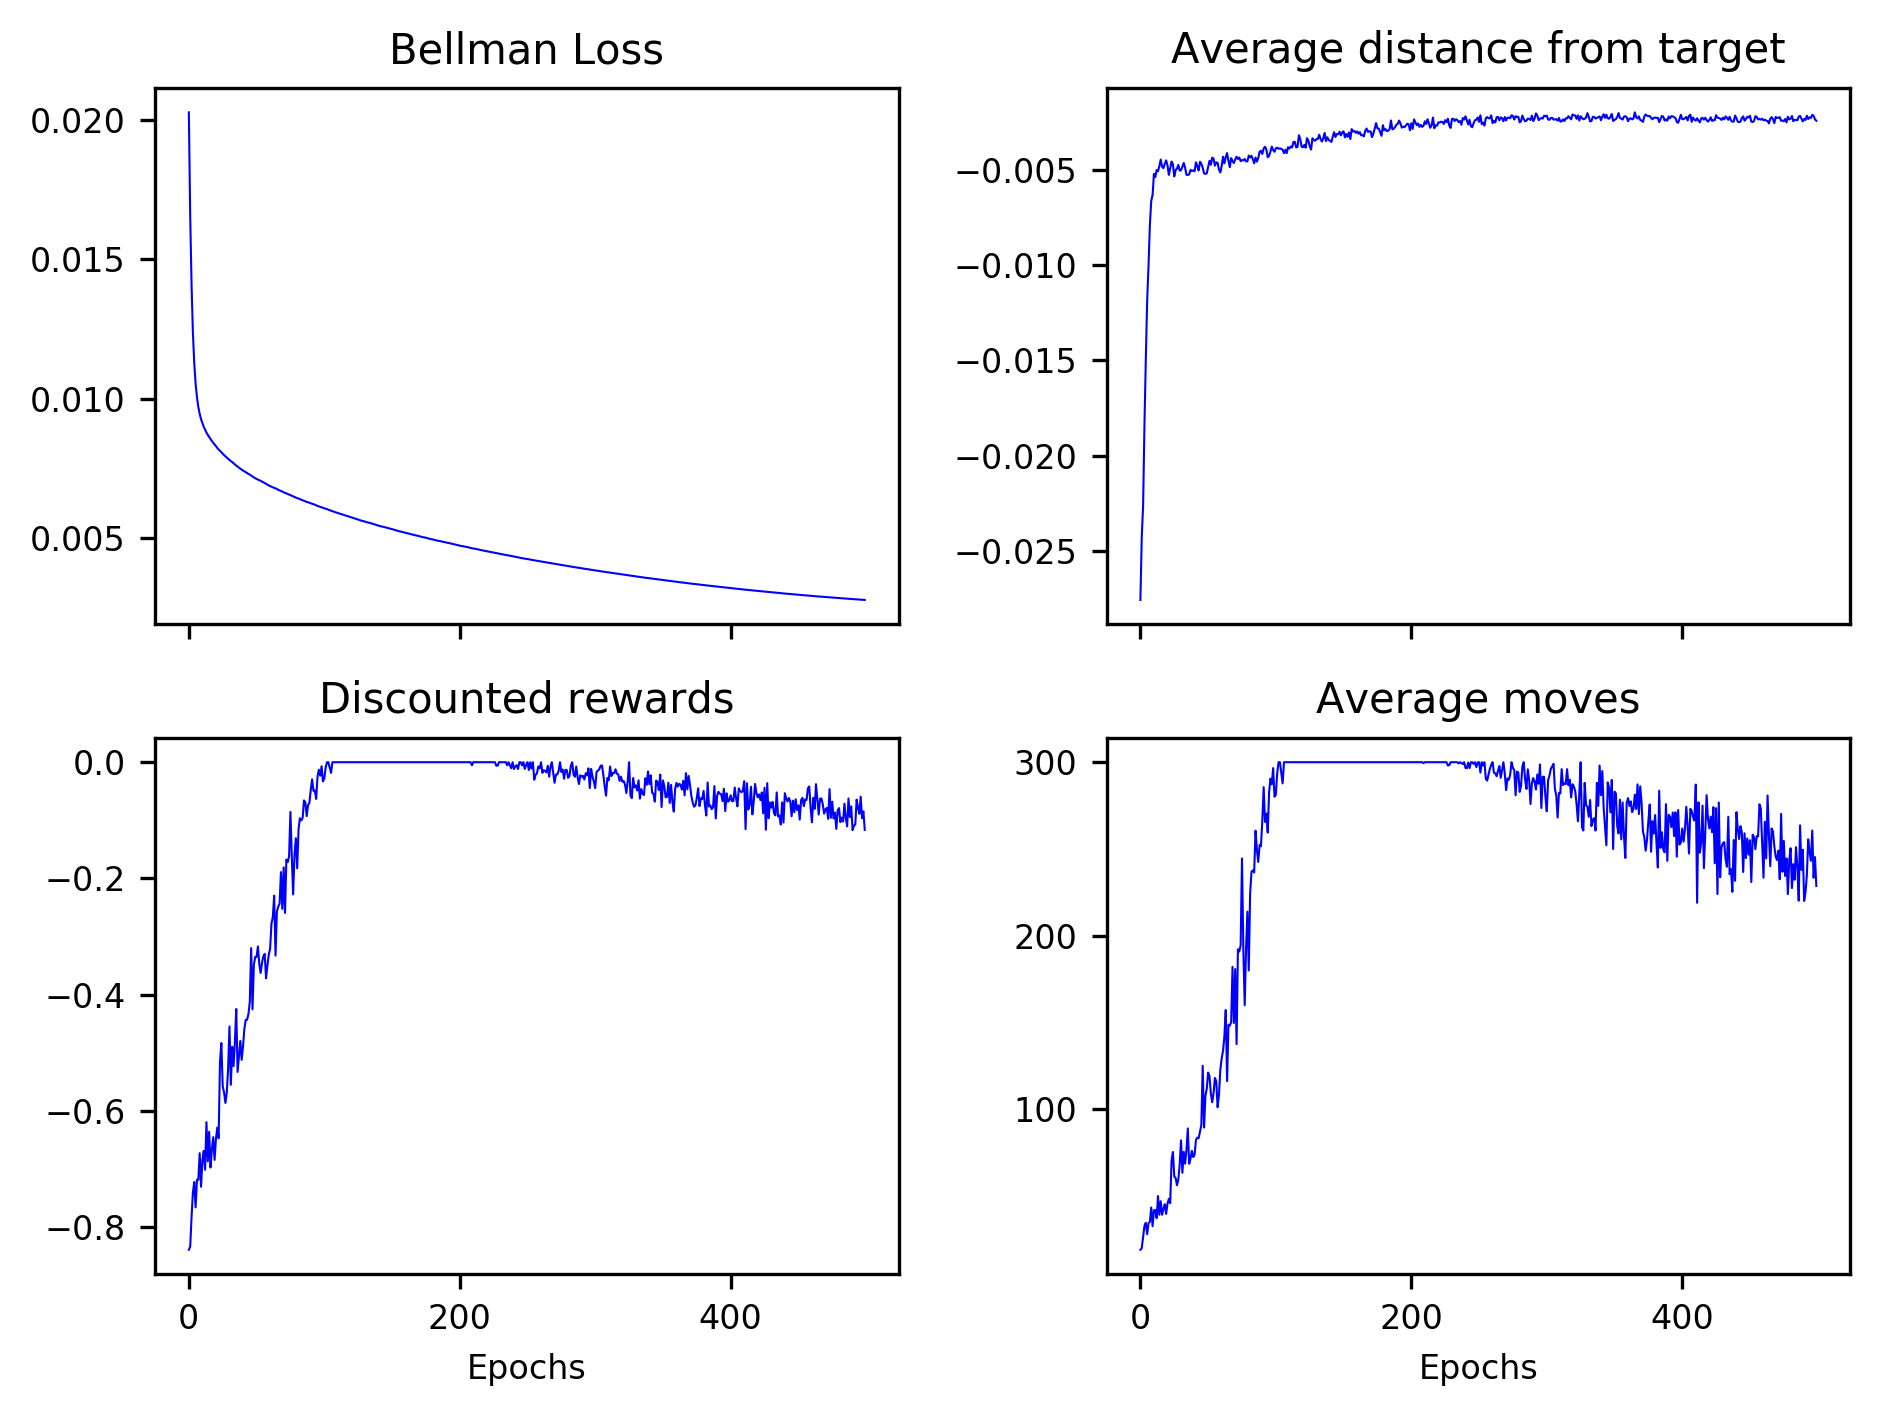
\includegraphics[height=8cm]{{figures/a3b_0.5}.png}
	\end{center}
    \caption{%
		Batch Q-learning with neural network with one hidden layer of 100 units. Learning rate = 0.5.
     }%
\end{figure}


\subsection{Online Q-learning}

The online Q-learning experiment was run 100 times with the following parameters: Learning rate: 0.01. A graph of the average reward and standard deviation is given below.

\begin{figure}[H]
	\begin{center}
     	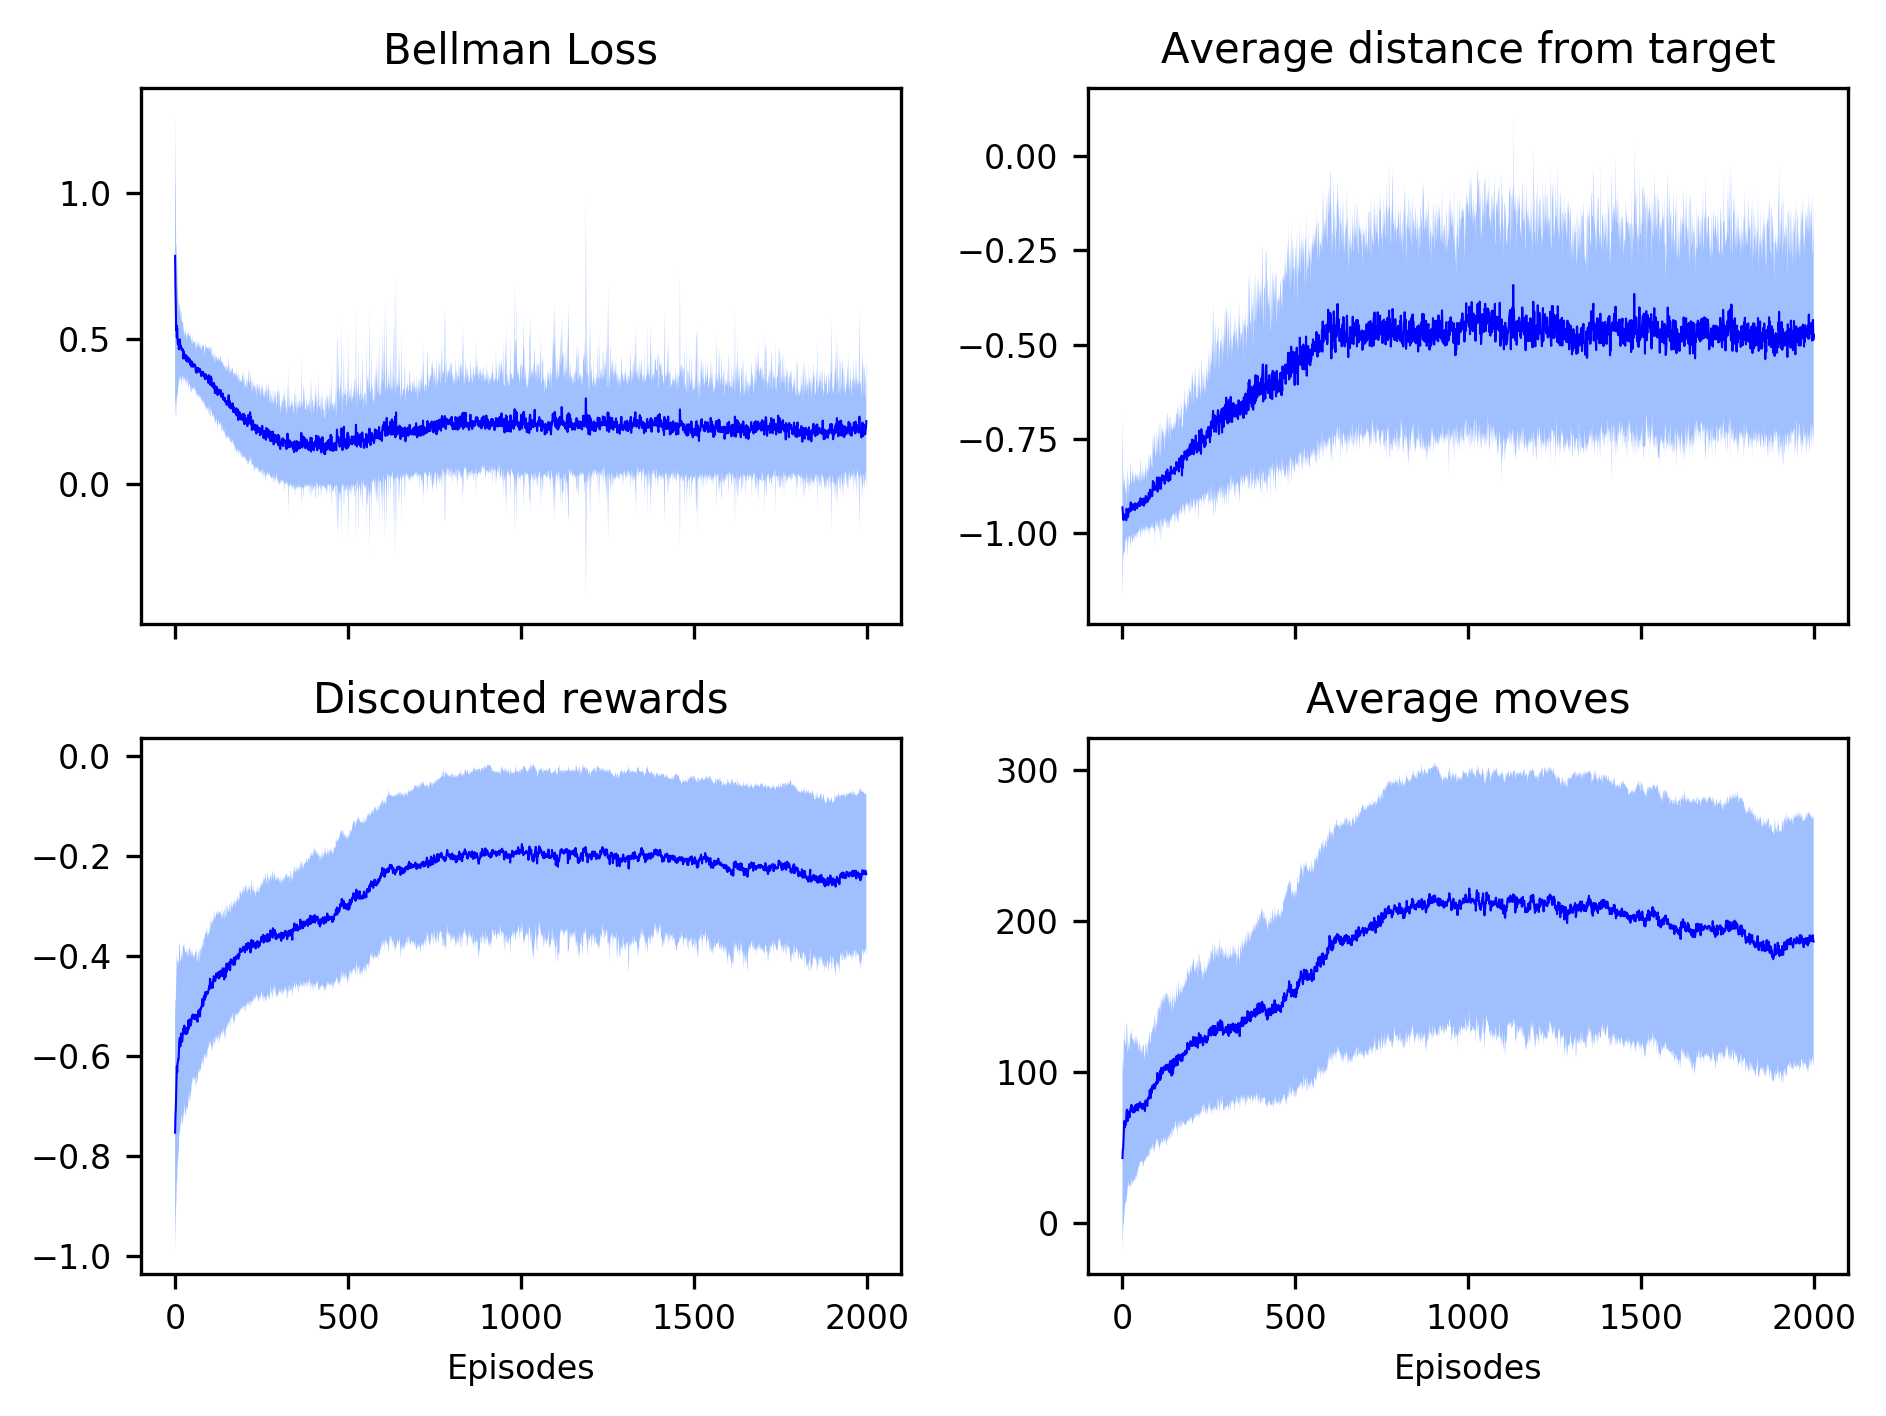
\includegraphics[height=10cm]{{figures/a4_0.01}.png}
	\end{center}
    \caption{%
		Online Q-learning with neural network with one hidden layer of 100 units, run 100 times. Dark blue line is average over these 100 trials. Light blue area is +/- 1 standard deviation. Learning rate = 0.01.
     }%
\end{figure}

We can see the typical test performance of this agent is about 200 moves, after it has been training on using an $\epsilon$-greedy ($\epsilon=0.05$) policy for approximately 1000 episodes. Also, since we can see that +1 standard deviation is almost 300 moves, it can be noted that at many points during these experiments, the agent actually succeeded at balancing the pole for 300 moves, particularly after being trained over 1000 episodes. The variance, however, is quite high, and a few times the agent even oscillated between 300 and 9 (not present in figures).

\newpage
\subsection{Changing the hidden layer}
We modified the above agent and ran the experiment one time each to observe any change in behaviour. The learning rate was 0.01.

\subsubsection{Fewer units (30)}
Given below is a graph using a hidden layer of 30 units.

\begin{figure}[H]
	\begin{center}
     	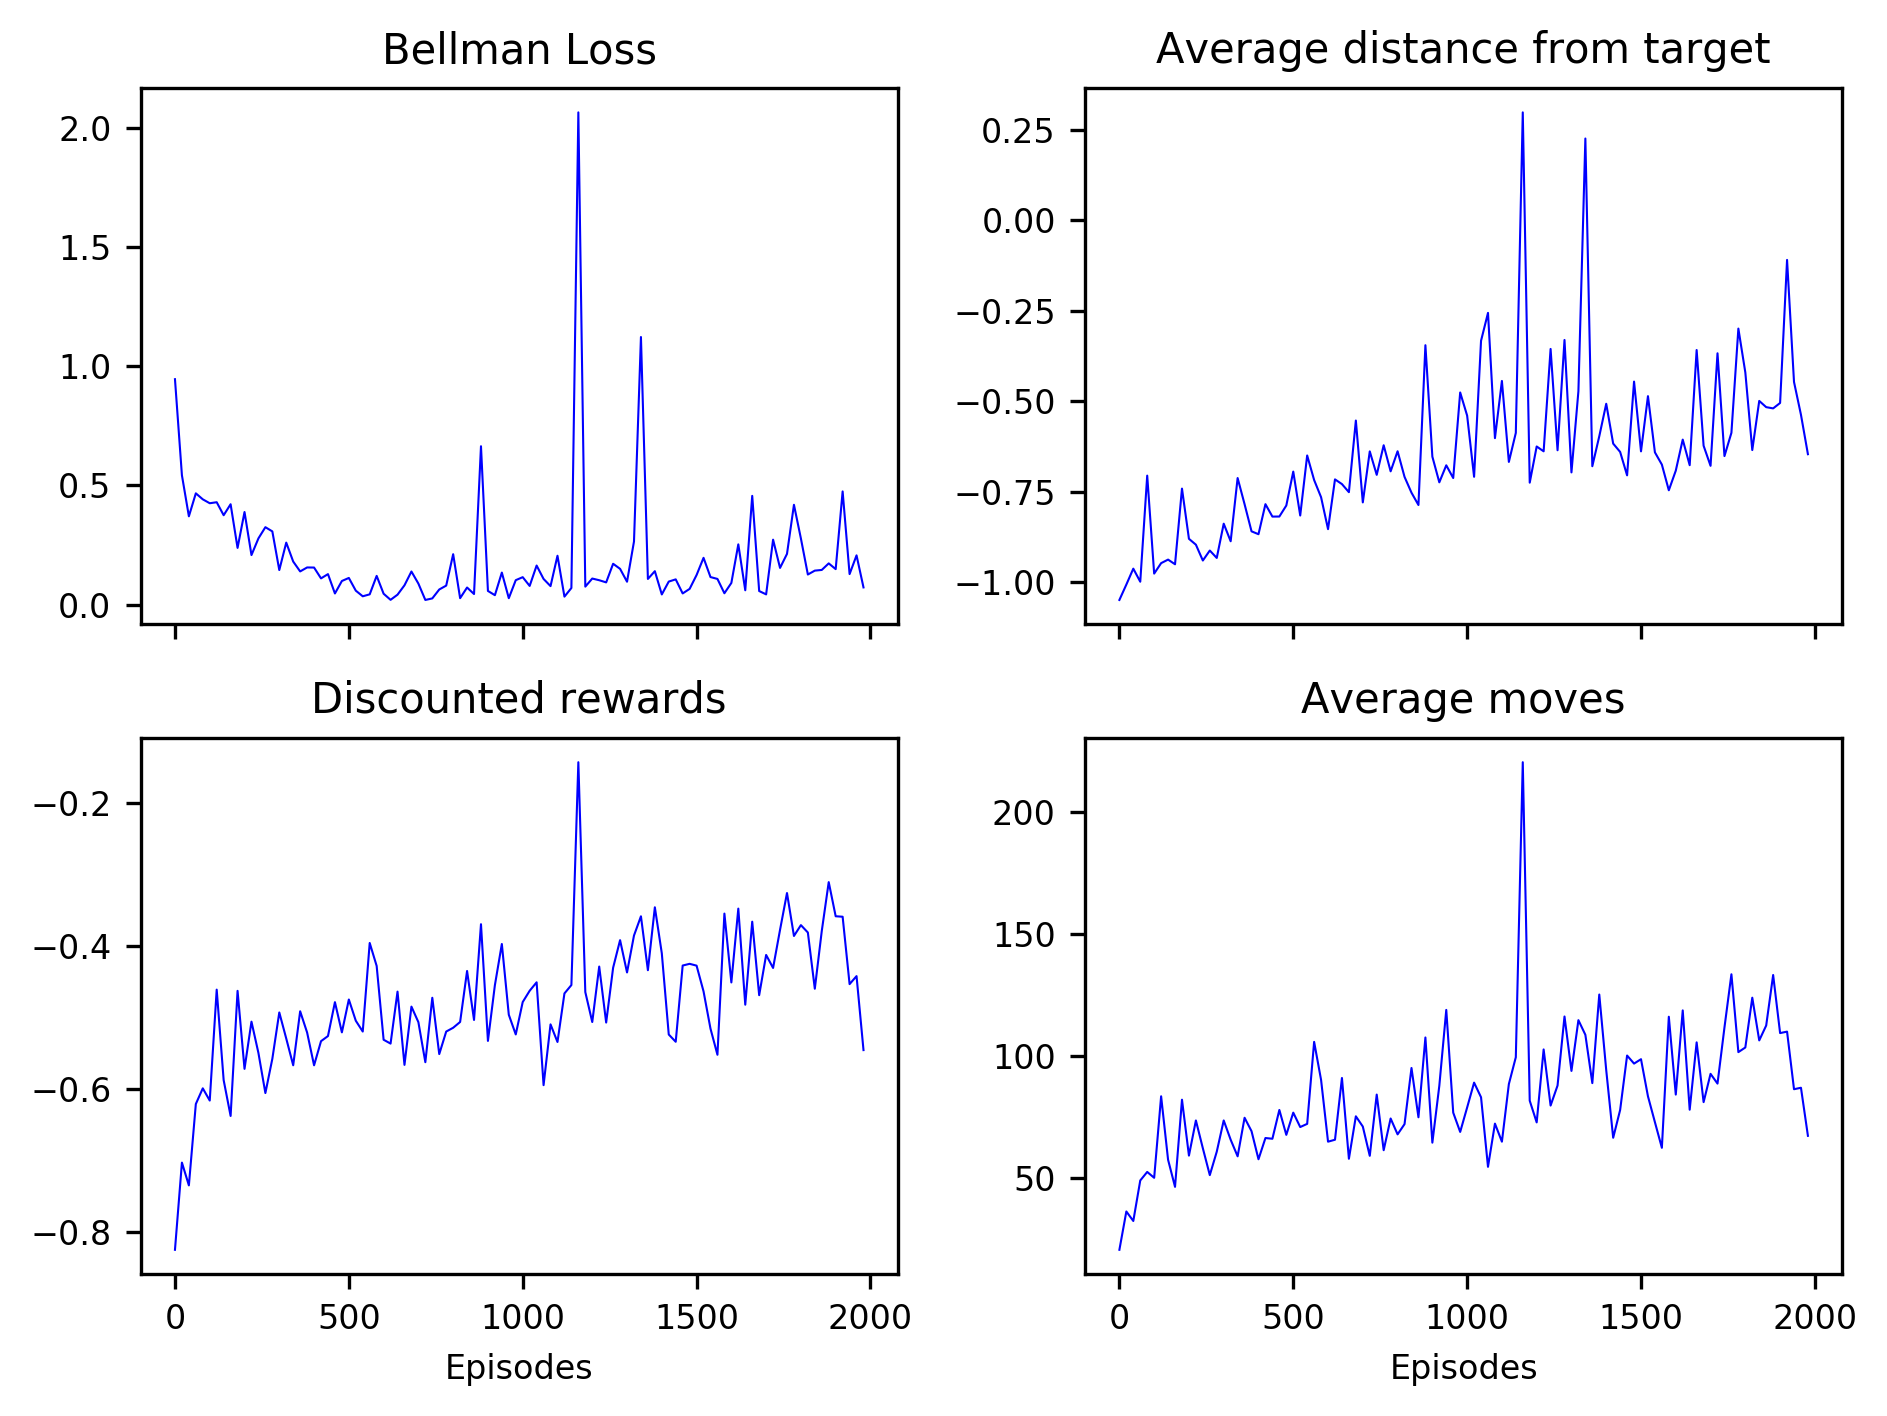
\includegraphics[height=10cm]{{figures/a5_30_0.01}.png}
	\end{center}
    \caption{%
		Online Q-learning with neural network with one hidden layer of 30 units. Learning rate = 0.01. Points are plotted every 20 episodes.
     }%
\end{figure}

Compared to the previous chart, it appears that this network fares worse. The average number of moves at test time appears to be around 100, even after 2000 episodes of training. However, one trial is not conclusive evidence that this network is unable to solve the problem, even through it is quantitatively less expressive than the network in section 1.4.
\newpage
\subsubsection{More units (1000)}
Given below is a graph using a hidden layer of 1000 units.

\begin{figure}[H]
	\begin{center}
     	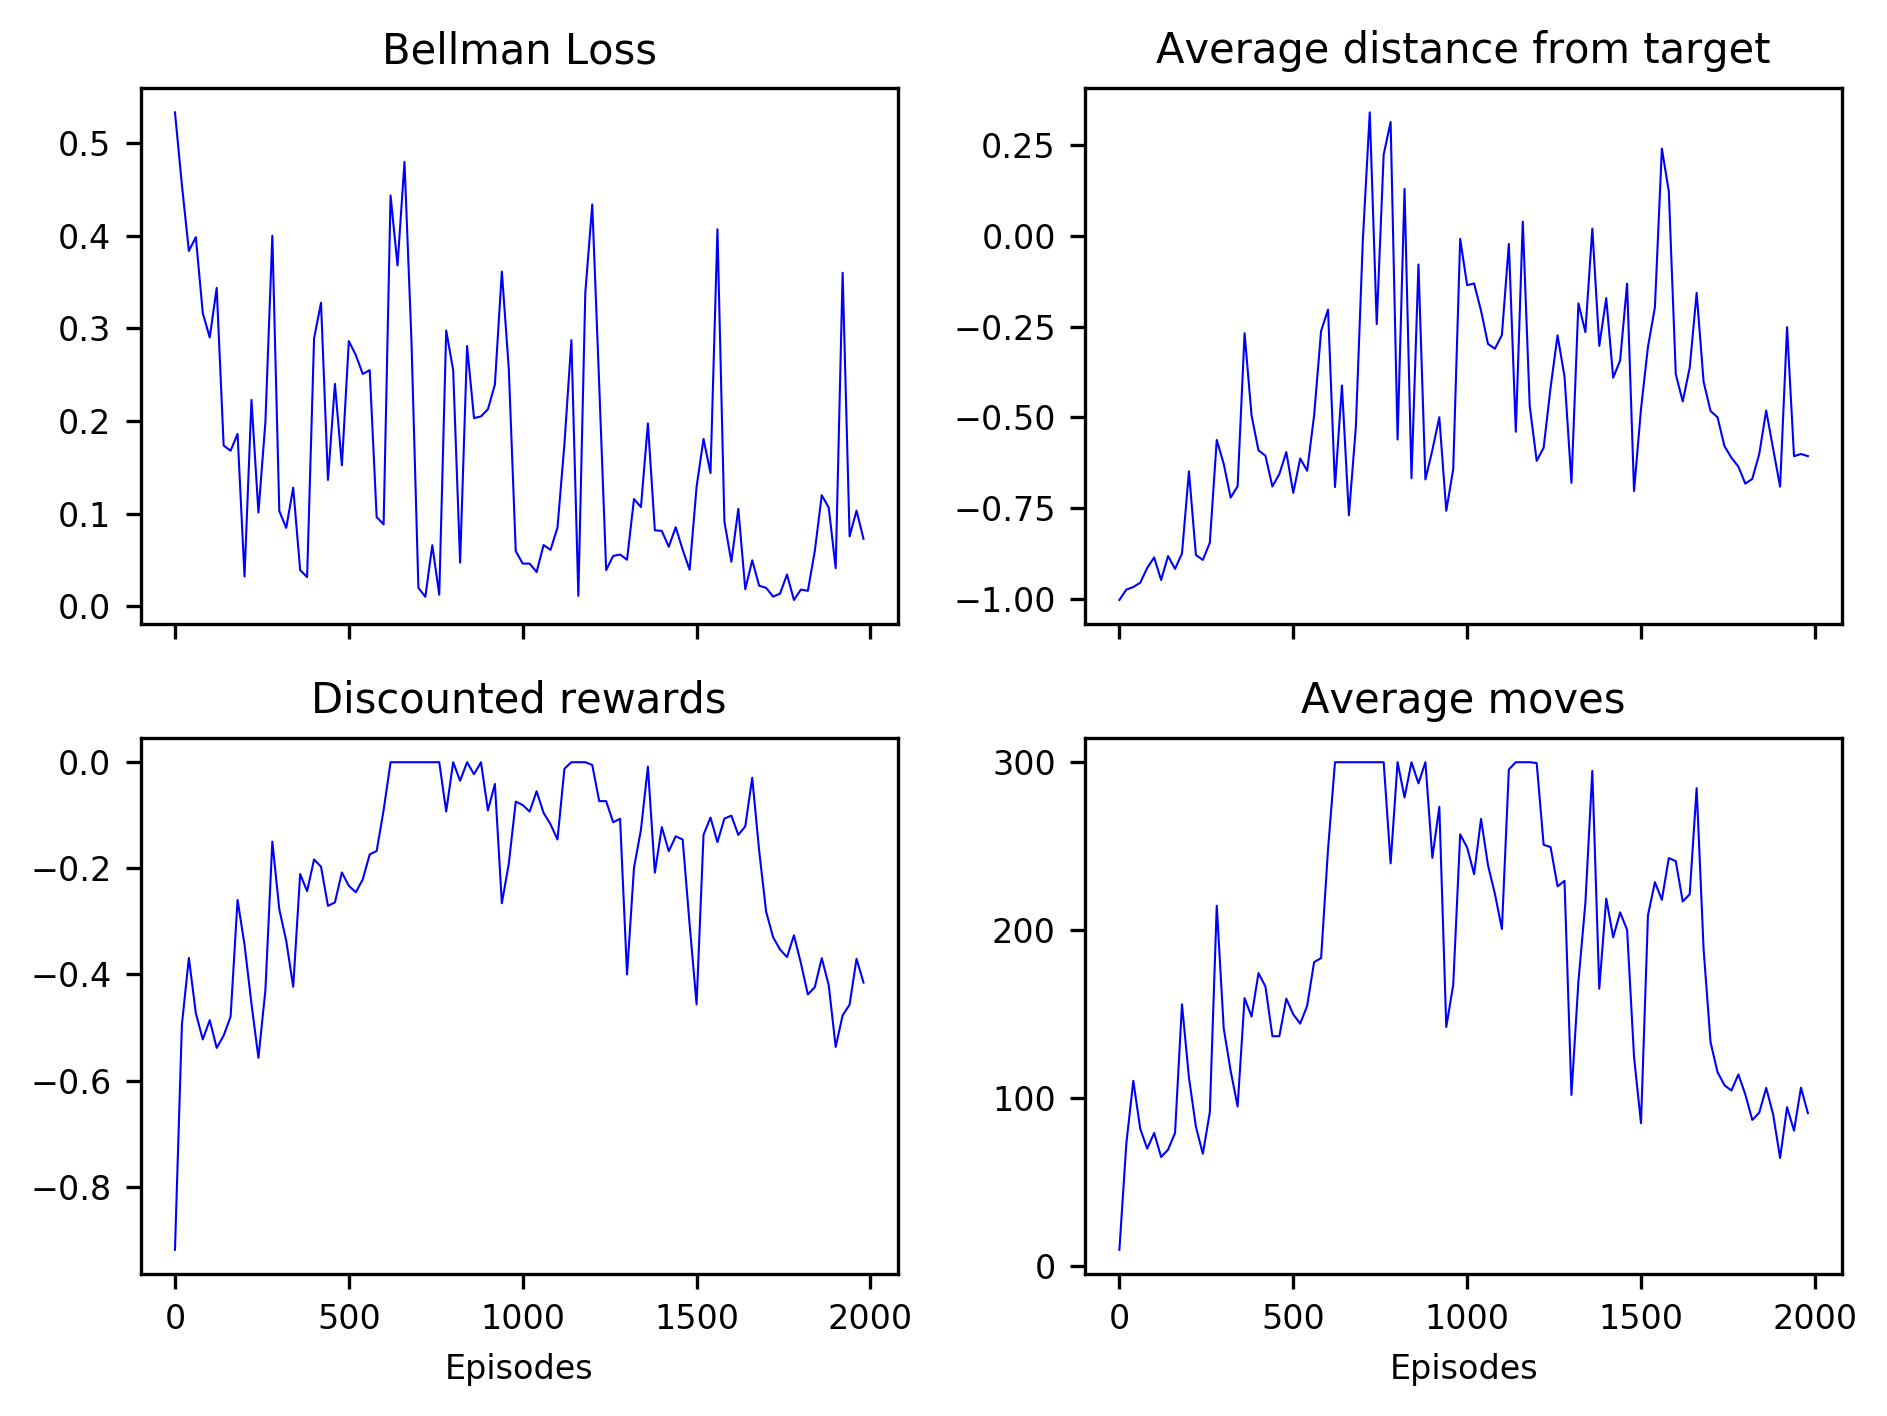
\includegraphics[height=10cm]{{figures/a5_1000_0.01}.png}
	\end{center}
    \caption{%
		Online Q-learning with neural network with one hidden layer of 1000 units. Learning rate = 0.01. Points are plotted every 20 episodes.
     }%
\end{figure}

Compared to the chart in section 1.4, it appears that this network performs a little better. It is able to solve the problem consistently for about 100 episodes from episodes \textasciitilde 650 and \textasciitilde 750. It also returns to this peak a few times during the whole trial. Again, one trial is not conclusive evidence that this network is better able to solve the problem, even through it is quantitatively more expressive than the network in section 1.4. We can also see from this graph that the learning of this algorithm can be unstable. This is possibly because of the learning rate being held at 0.01 as in the previous experiments. The output layer can now have potentially 10x the magnitude when compared to the network in 1.4, and this might be a source of unwanted, unstable agent behaviour. This would explain the unusual Bellman loss curve as well.

\newpage
\subsection{Adding experiece replay}
Given below is a graph of the behaviour of an agent from Q4 augmented with an experience replay buffer of size 10000. The learning rate is 0.01. Mini-batch size was set to 512. The experience replay buffer size was obtained through an exhaustive search over the values \{$n \times 2000 : 0 < n < 8$\}.

\begin{figure}[H]
    \caption{%
		Online Q-learning with an experience replay buffer of 10000. Learning rate = 0.01. Points are plotted every 20 episodes.
     }%
	\begin{center}
     	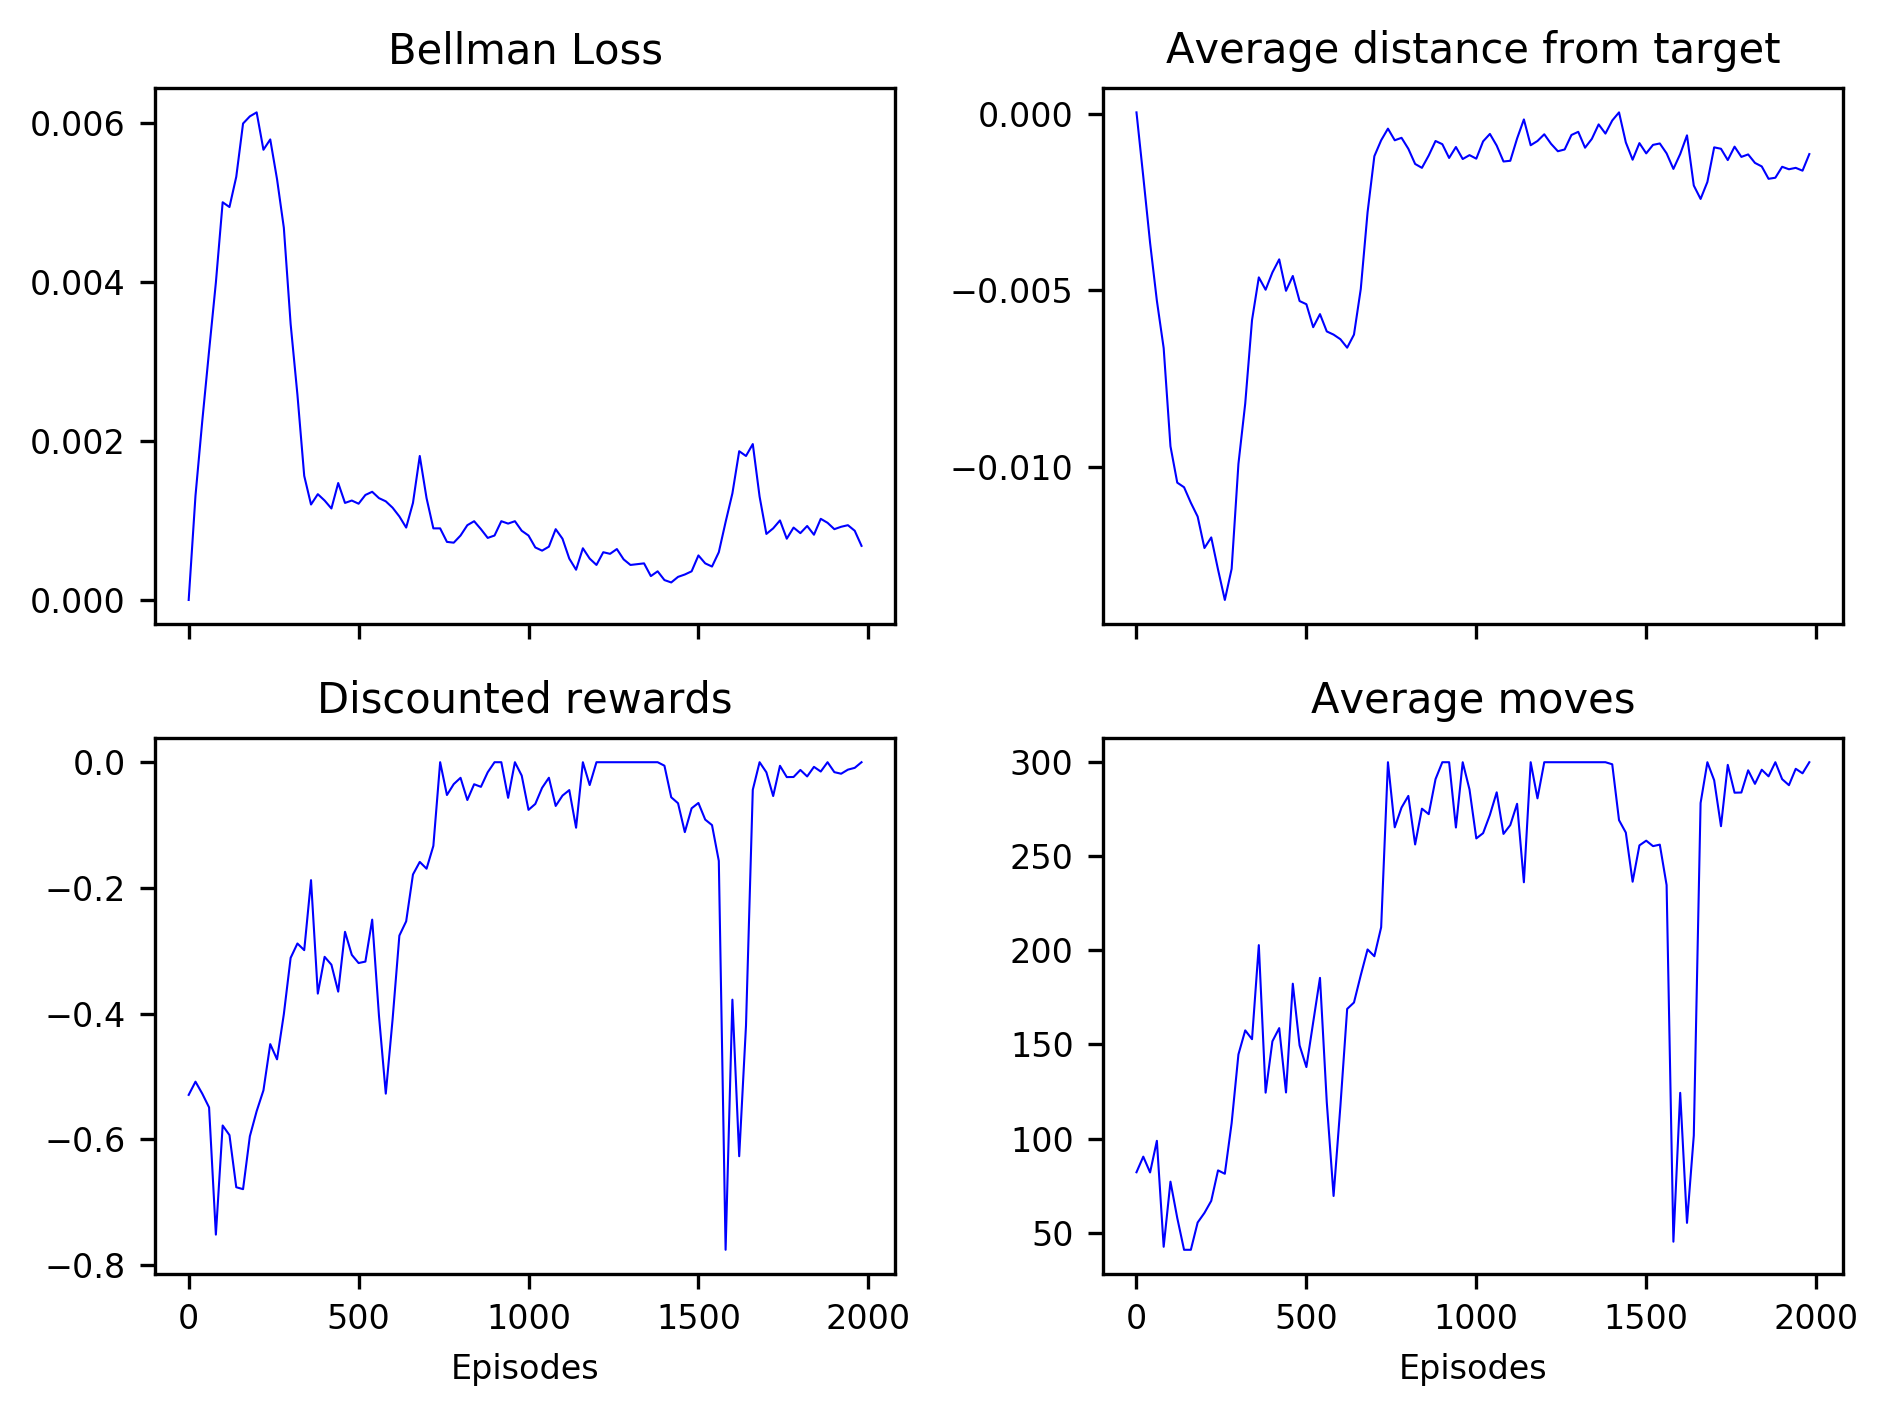
\includegraphics[height=10cm]{{figures/a6_0.01_10000}.png}
	\end{center}
\end{figure}

From the graph it is clear that experience replay significantly helps the learning process. The agent is able to successfully balance the poll for nearly one-fourth of the episodes. However, the agent can still un-learn, as it does almost catastrophically shortly after 1500 episodes.
\newpage
\subsection{Adding a target network}
The last agent was modified to include a target network, which was updated to the current network every 5 episodes. The learning rate used is 0.01. Its behaviour is graphed below.

\begin{figure}[H]
    \caption{%
		Online Q-learning with an experience replay buffer of 10000 and a target network being updated every 5 episodes. Learning rate = 0.01. Points are plotted every 20 episodes.
     }%
	\begin{center}
     	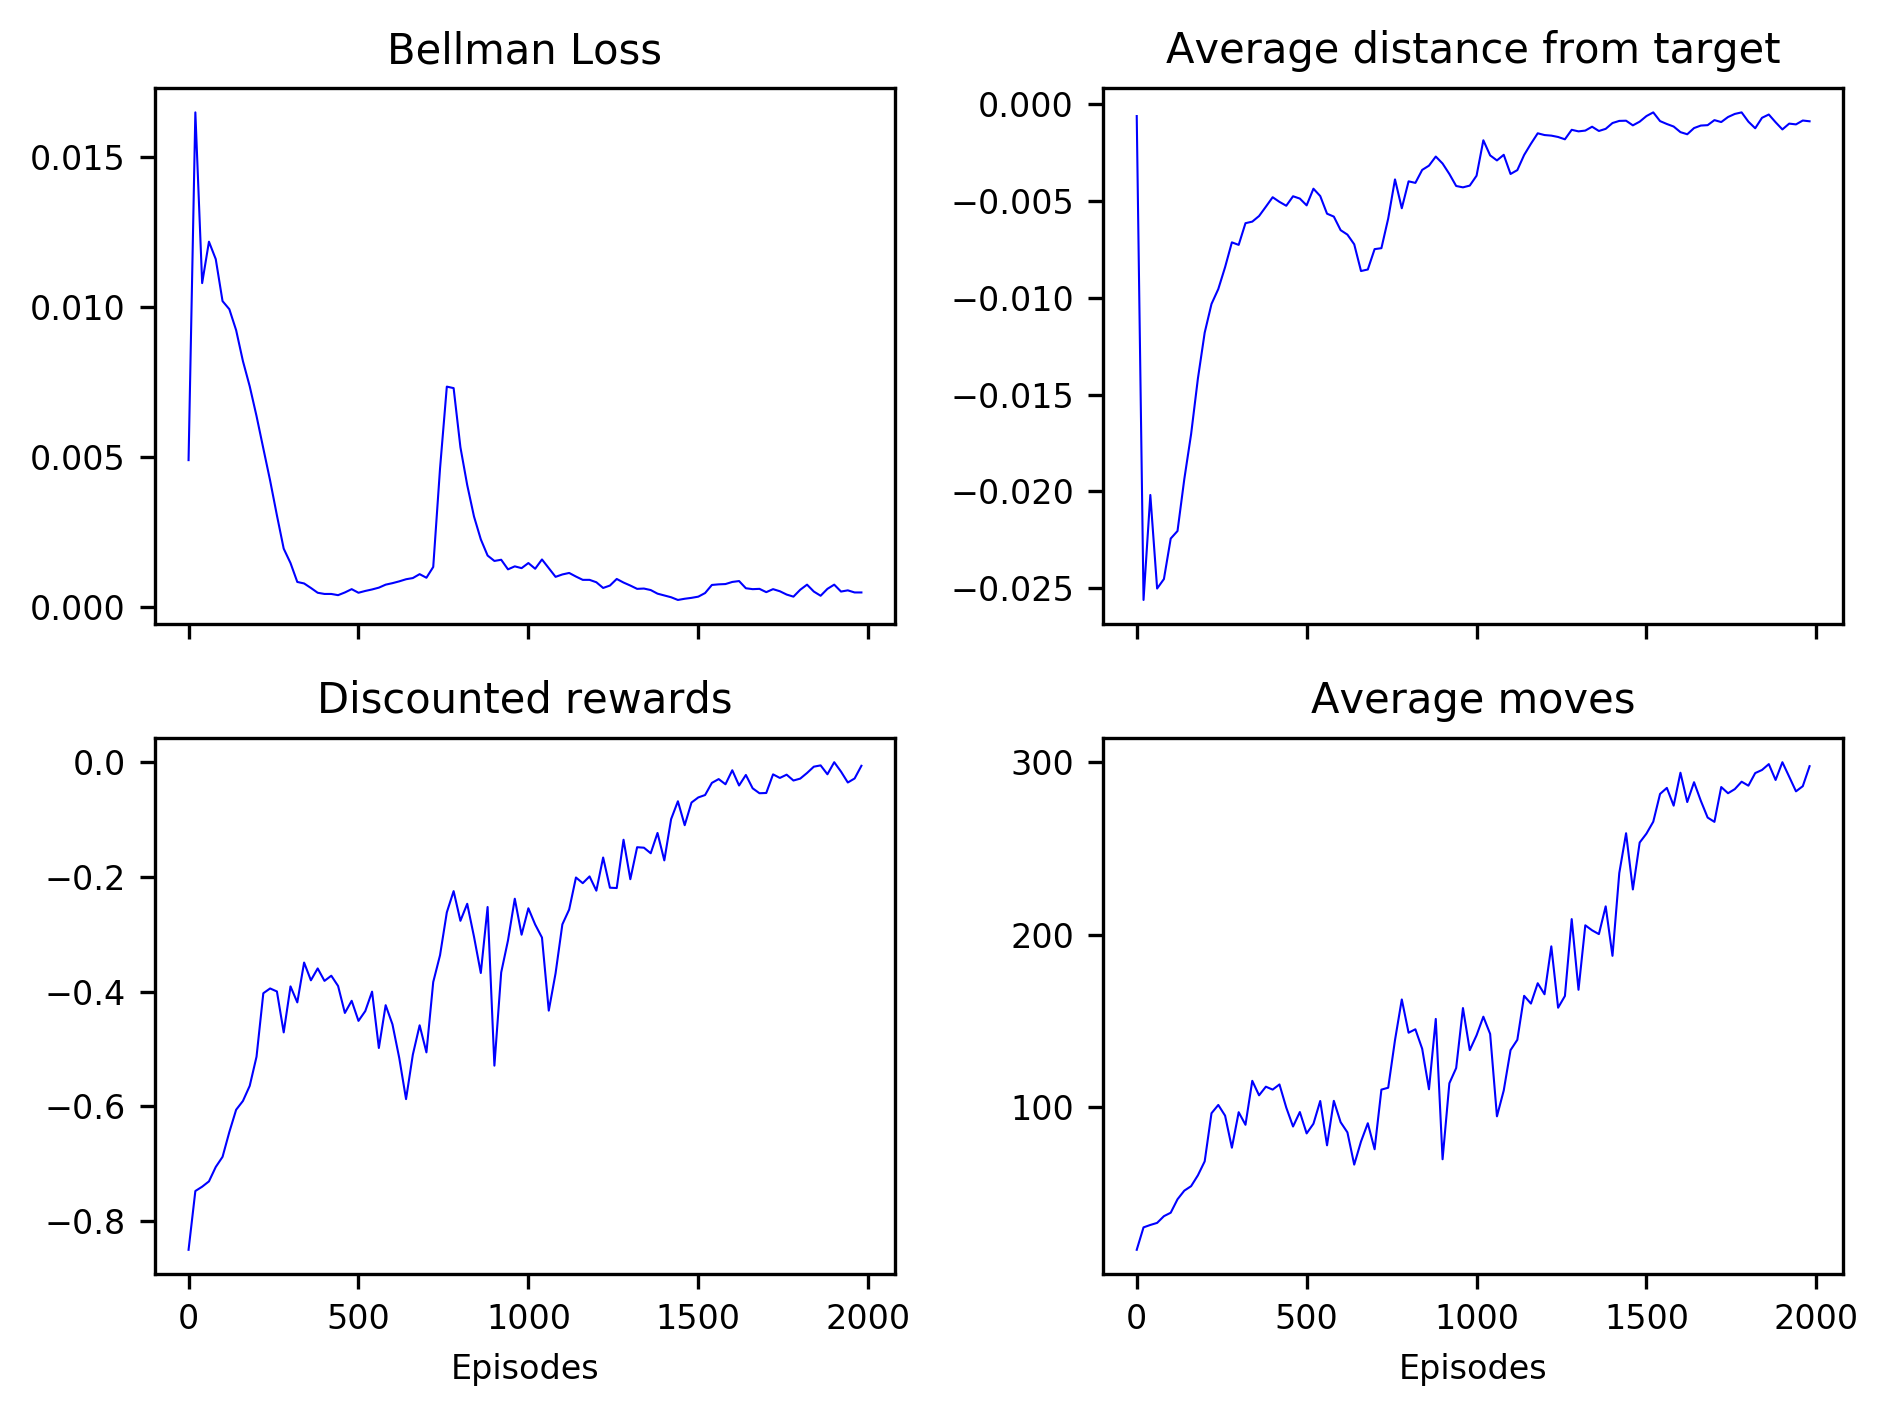
\includegraphics[height=10cm]{{figures/a7_0.01_10000}.png}
	\end{center}
\end{figure}

Two key differences between this graph and the one from section 1.6 are 1) This agent learns a little slower, however, 2) it doesn't forget catastrophically, and does not drop far away the peaks it reaches. The loss curves also look less jagged than those in section 1.6.

\newpage
\subsection{Implementing a SARSA agent}
We started with the agent from Q4 and modified it to learn as per the SARSA algorithm. The learning rate used is 0.01. Its behaviour is graphed below.

\begin{figure}[H]
    \caption{%
		SARSA learning agent. Learning rate = 0.01. Points are plotted every 20 episodes.
     }%
	\begin{center}
     	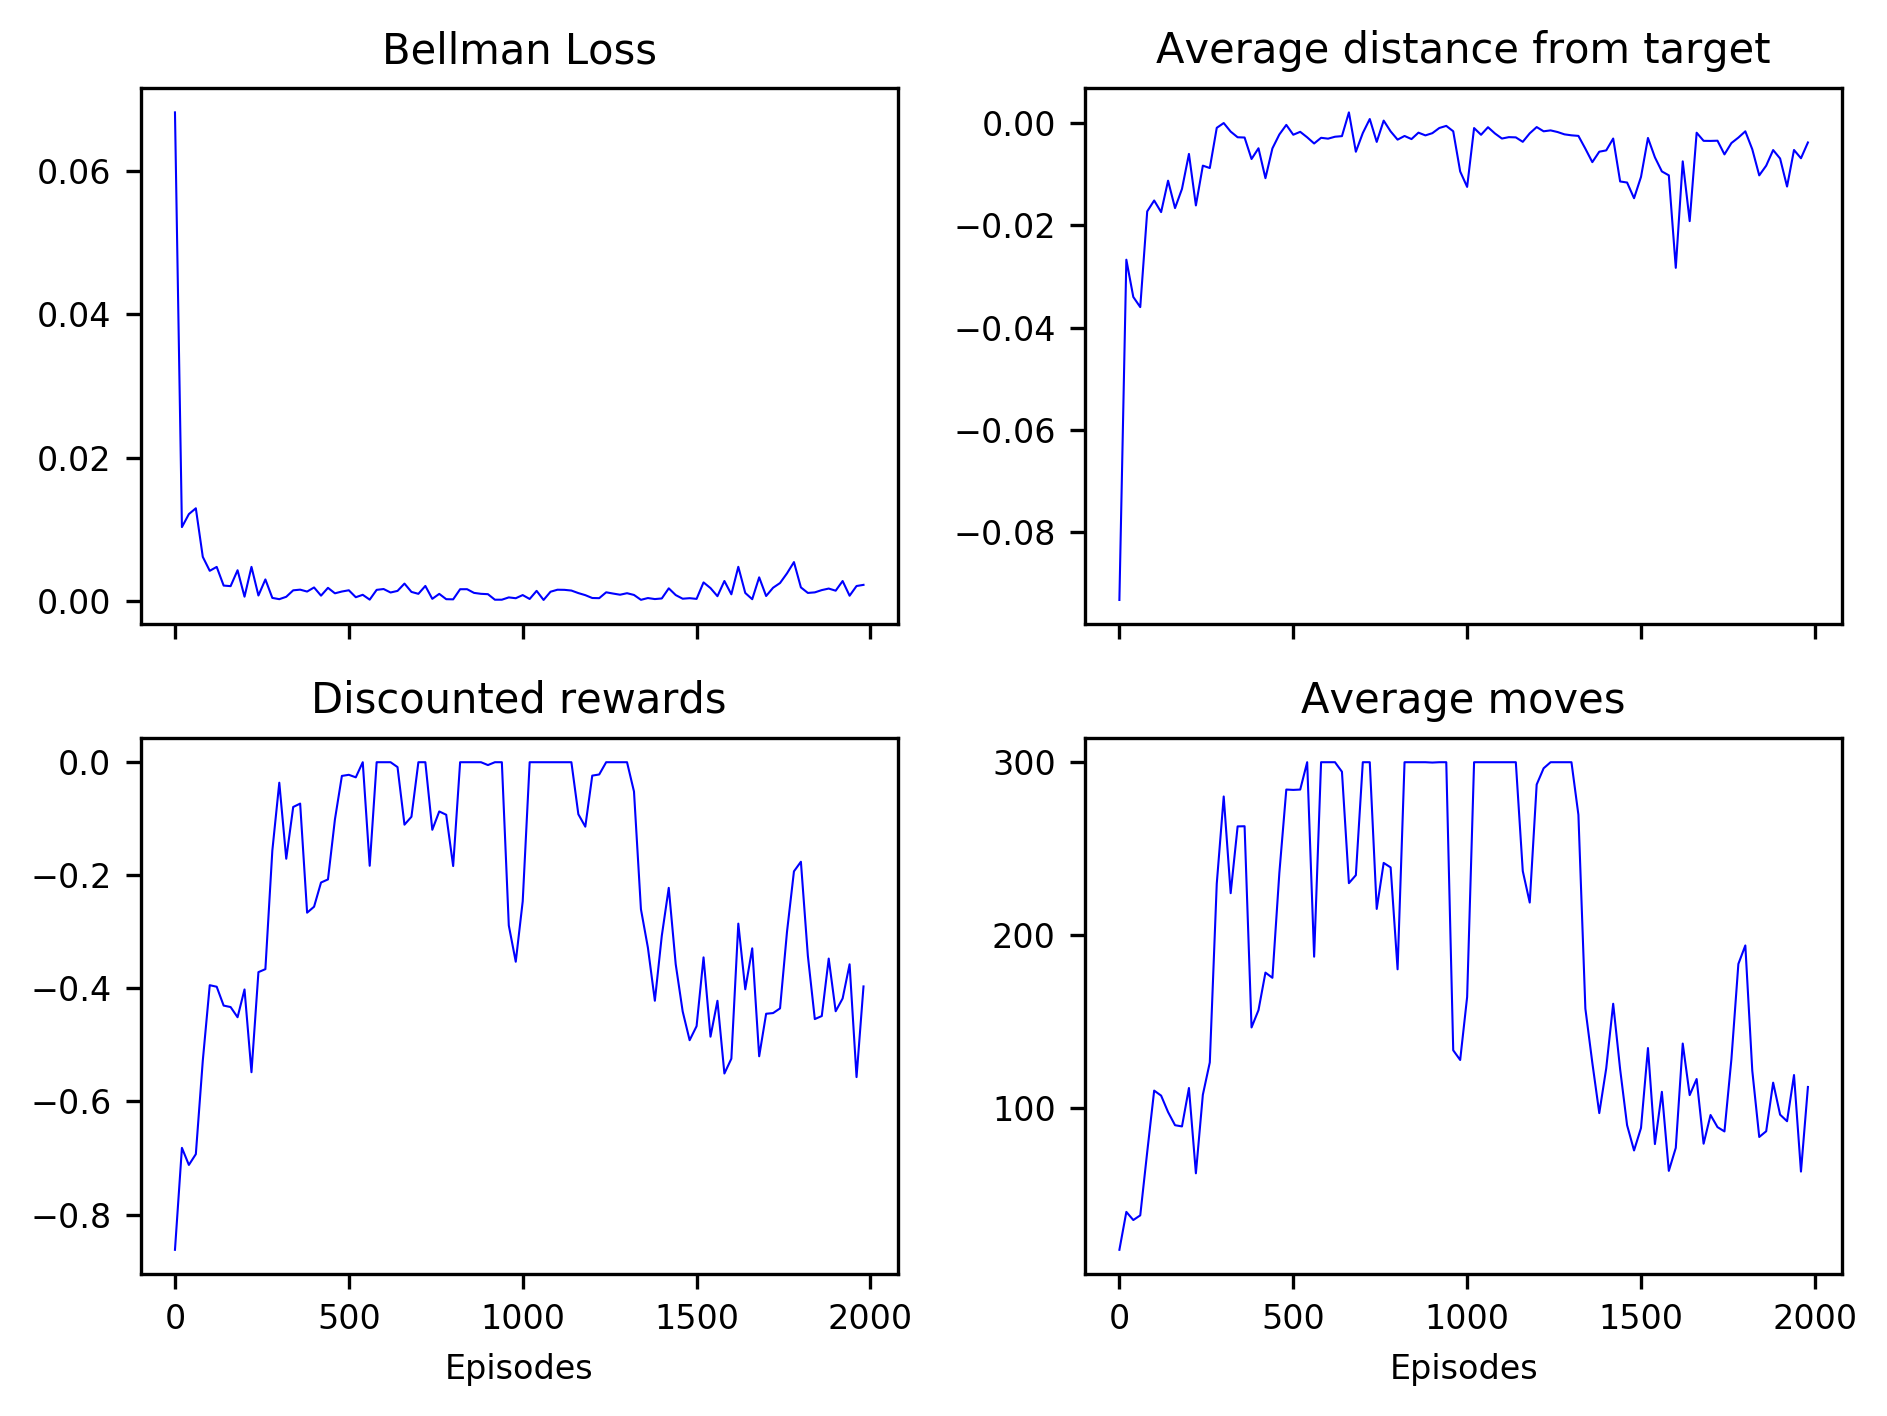
\includegraphics[height=10cm]{{figures/a8_0.01}.png}
	\end{center}
\end{figure}

In comparison to 1.4, 1.5, 1.6 and 1.7, this SARSA agent seems to perform the best, with the one flaw that it also regularly catastrophically forgets after demonstrating strong performance for 50 to 100 episodes at a time. In this trial, after 1500 epsiodes it falls into a zone of sub-optimal performance, perhaps due to a high learning rate.\\

Additional trials of this experiment(not graphed) showed similar strong performance with periodic forgetfulness on the part of the agent. 

\newpage
\section{Problem B: Atari Games}
For these problems, the following specifications for the world state were implemented.
\begin{itemize}
\item Observations were preprocessed from $210 \times 160 \times 3$ to either $60 \times 60 \times 1$, $40 \times 40 \times 1$, or $28 \times 28 \times 1$
\item Rewards were clipped to -1, 0 or 1
\item For the game \texttt{Pong}, images were thresholded to black and white before shrinking
\item Images were clipped to the dynamic areas of the screen
\end{itemize}
Further, the following features were implemented.
\begin{itemize}
\item Where possible, the agents were trained to 2,000,000 steps
\item An empty experience buffer of 400,000 transitions was created
\item The Q function was approximated using a two-stage convolutional neural network
\item Mini-batch sizes of 32 were used during training
\item RMSPropOptimizer was used for training the agent
\item Learning rates in \{0.00001, 0.0001, 0.001, 0.01, 0.1\} were tried
\item Performance of the agent was evaluated every 50,000 steps
\item Experiments were run with 1) an $\epsilon$ of 0.1 and 2) a decaying $\epsilon$ from 1 to 0.1 over the the first 500,000 steps.
\end{itemize}

\subsection{Random policy}
An agent following a random policy was evaluated on 100 runs of each game. Mean and standard deviations are reported below. No learning rate was required for this experiment.\\

\texttt{
Game : Pong-v3 \newline
Possible actions : 6 \newline
Evaluation over 100 episodes \newline
Avg steps: 1260.15 \quad\quad\quad\quad\quad\quad\quad  Standard deviation: 164.947165783 \newline
Avg tot rew: -20.13 \quad\quad\quad\quad\quad\quad\quad  Standard deviation: 0.955562661472 \newline
Avg disc rew: -0.889193101266 \quad\quad Standard deviation: 0.319726787337 \newline
}

\texttt{
Game : MsPacman-v3 \newline
Possible actions : 9 \newline
Evaluation over 100 episodes \newline
Avg steps: 646.66 \quad\quad\quad\quad\quad\quad\quad\quad  Standard deviation: 102.025998647 \newline
Avg tot rew: 20.3 \quad\quad\quad\quad\quad\quad\quad\quad Standard deviation: 6.63551053047 \newline
Avg disc rew: 2.45008162806 \quad\quad\quad  Standard deviation: 0.668114730719\newline
}

\texttt{
Game : Boxing-v3 \newline
Possible actions : 18 \newline
Evaluation over 100 episodes \newline
Avg steps: 2381.73 \quad\quad\quad\quad\quad\quad\quad\quad\quad Standard deviation: 12.9459298623 \newline
Avg tot rew: 1.69 \quad\quad\quad\quad\quad\quad\quad\quad\quad  Standard deviation: 3.76216692878 \newline
Avg disc rew: -0.208223222938 \quad\quad\quad  Standard deviation: 0.99363394195 \newline
}


\subsection{Untrained Q-network}
An agent following a greedy policy on an initialised but untrained Q-network was evaluated on 100 runs of each game. Mean and standard deviations are reported below. No learning rate was required for this experiment.\\

\texttt{
Game : Pong-v3 \newline
Possible actions : 6 \newline
Evaluation over 100 episodes \newline
Avg steps: 1020.06 \quad\quad\quad\quad\quad\quad\quad\quad Standard deviation: 8.65658131135 \newline
Avg tot rew: -21.0 \quad\quad\quad\quad\quad\quad\quad\quad Standard deviation: 0.0 \newline
Avg disc rew: -1.12266604771 \quad\quad\quad Standard deviation: 0.0284774340357 \newline
}

\texttt{
Game : MsPacman-v3 \newline
Possible actions : 9 \newline
Evaluation over 100 episodes \newline
Avg steps: 458.0 \quad\quad\quad\quad\quad\quad\quad\quad\quad Standard deviation: 5.06557005677 \newline
Avg tot rew: 6.0 \quad\quad\quad\quad\quad\quad\quad\quad\quad Standard deviation: 0.0 \newline
Avg disc rew: 2.1784172183 \quad\quad\quad\quad Standard deviation: 0.0544610419163 \newline
}

\texttt{
Game : Boxing-v3 \newline
Possible actions : 18 \newline
Evaluation over 100 episodes \newline
Avg steps: 2381.73 \quad\quad\quad\quad\quad\quad\quad\quad Standard deviation: 12.9459298623 \newline
Avg tot rew: -25.0 \quad\quad\quad\quad\quad\quad\quad\quad Standard deviation: 0.0 \newline
Avg disc rew: -0.373366658935 \quad\quad\quad Standard deviation: 0.0166110046567 \newline
}

As we can see, the performance of this agent is different from the agent under a random policy from Q1. Our first observation is that the standard deviation for total reward is always 0. This implies that the untrained Q-learning agent takes the same actions every single time regardless of stochasticity in the environment and the inputs. This is expected because the untrained agent would most likely have weights that cannot give meaningful Q values; it is therefore possible that the Q values are so far away from each other, that their order from maximum to minimum is not affected by small changes in input state, and hence would take the same actions every time in similar states. Secondly, the untrained agent seems to perform worse than the random agent. This is because the random agent on average takes several different moves, allowing it to turn down corners in Ms Pacman, or occasionally return the ball and score in Pong, which our untrained Q-learning agent does not do.\\

\subsection{Training agents to play Atari games}

Presented below are graphs of Bellman loss = $0.5 \times \delta^2$, as well as averaged $\delta$ over the length of an episode, for each episode during training, for three Atari games.

\subsubsection{Pong}
After hyperparameter optimisation using grid-search, the best performing agent was selected. The image was downsampled to $60 \times 60 \times 1$; the learning rate chosen was 0.00001; $\epsilon$ was decayed from 1 to 0.1 over the first 500,000 episodes. The agent was trained for 2,000,000 steps.

\begin{figure}[H]
    \caption{%
		Bellman loss and distance from target for agent while learing to play Pong
     }%
	\begin{center}
     	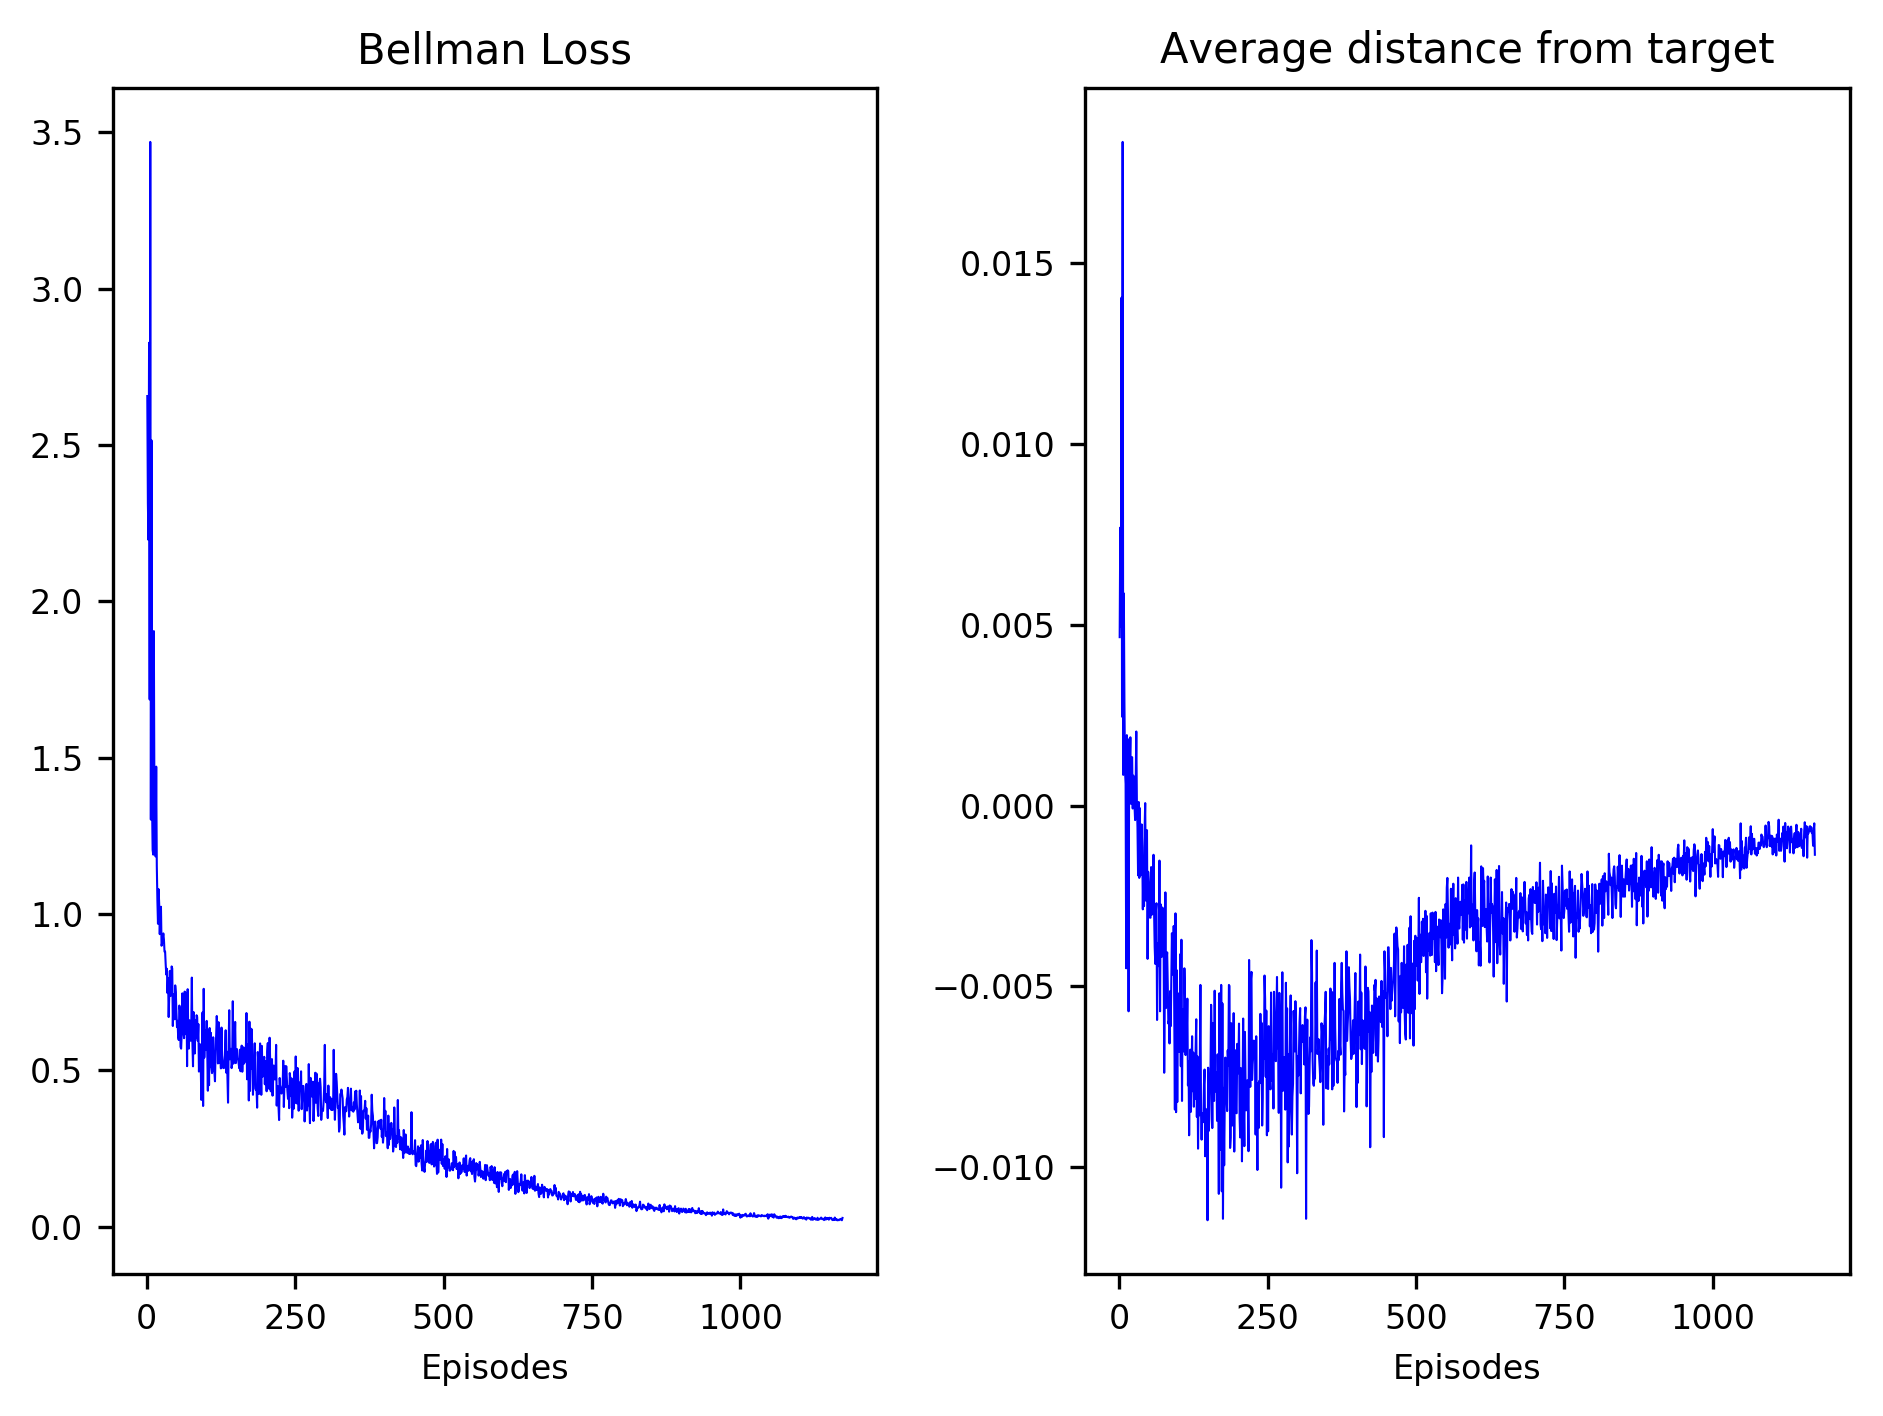
\includegraphics[height=10cm]{{figures/b34_0_0.00001_0_train}.png}
	\end{center}
\end{figure}

The Bellman Loss resembles a supervised learning curve closely. The Average distance from target curve dips for the first 200 episodes; we think this is because during this time, the algorithm is learning from experience drawn from a largely random policy, while $\epsilon$ decay from 1 to 0.1 over the first 500,000 steps.

\subsubsection{Ms Pacman}
After hyperparameter optimisation using grid-search, the best performing agent was selected. The image was downsampled to $60 \times 60 \times 1$; the learning rate chosen was 0.00001; $\epsilon$ was set to 0.1 throughout training. The agent was trained for 1,000,000 steps.

\begin{figure}[H]
    \caption{%
		Bellman loss and distance from target for agent while learing to play Ms Pacman
     }%
	\begin{center}
     	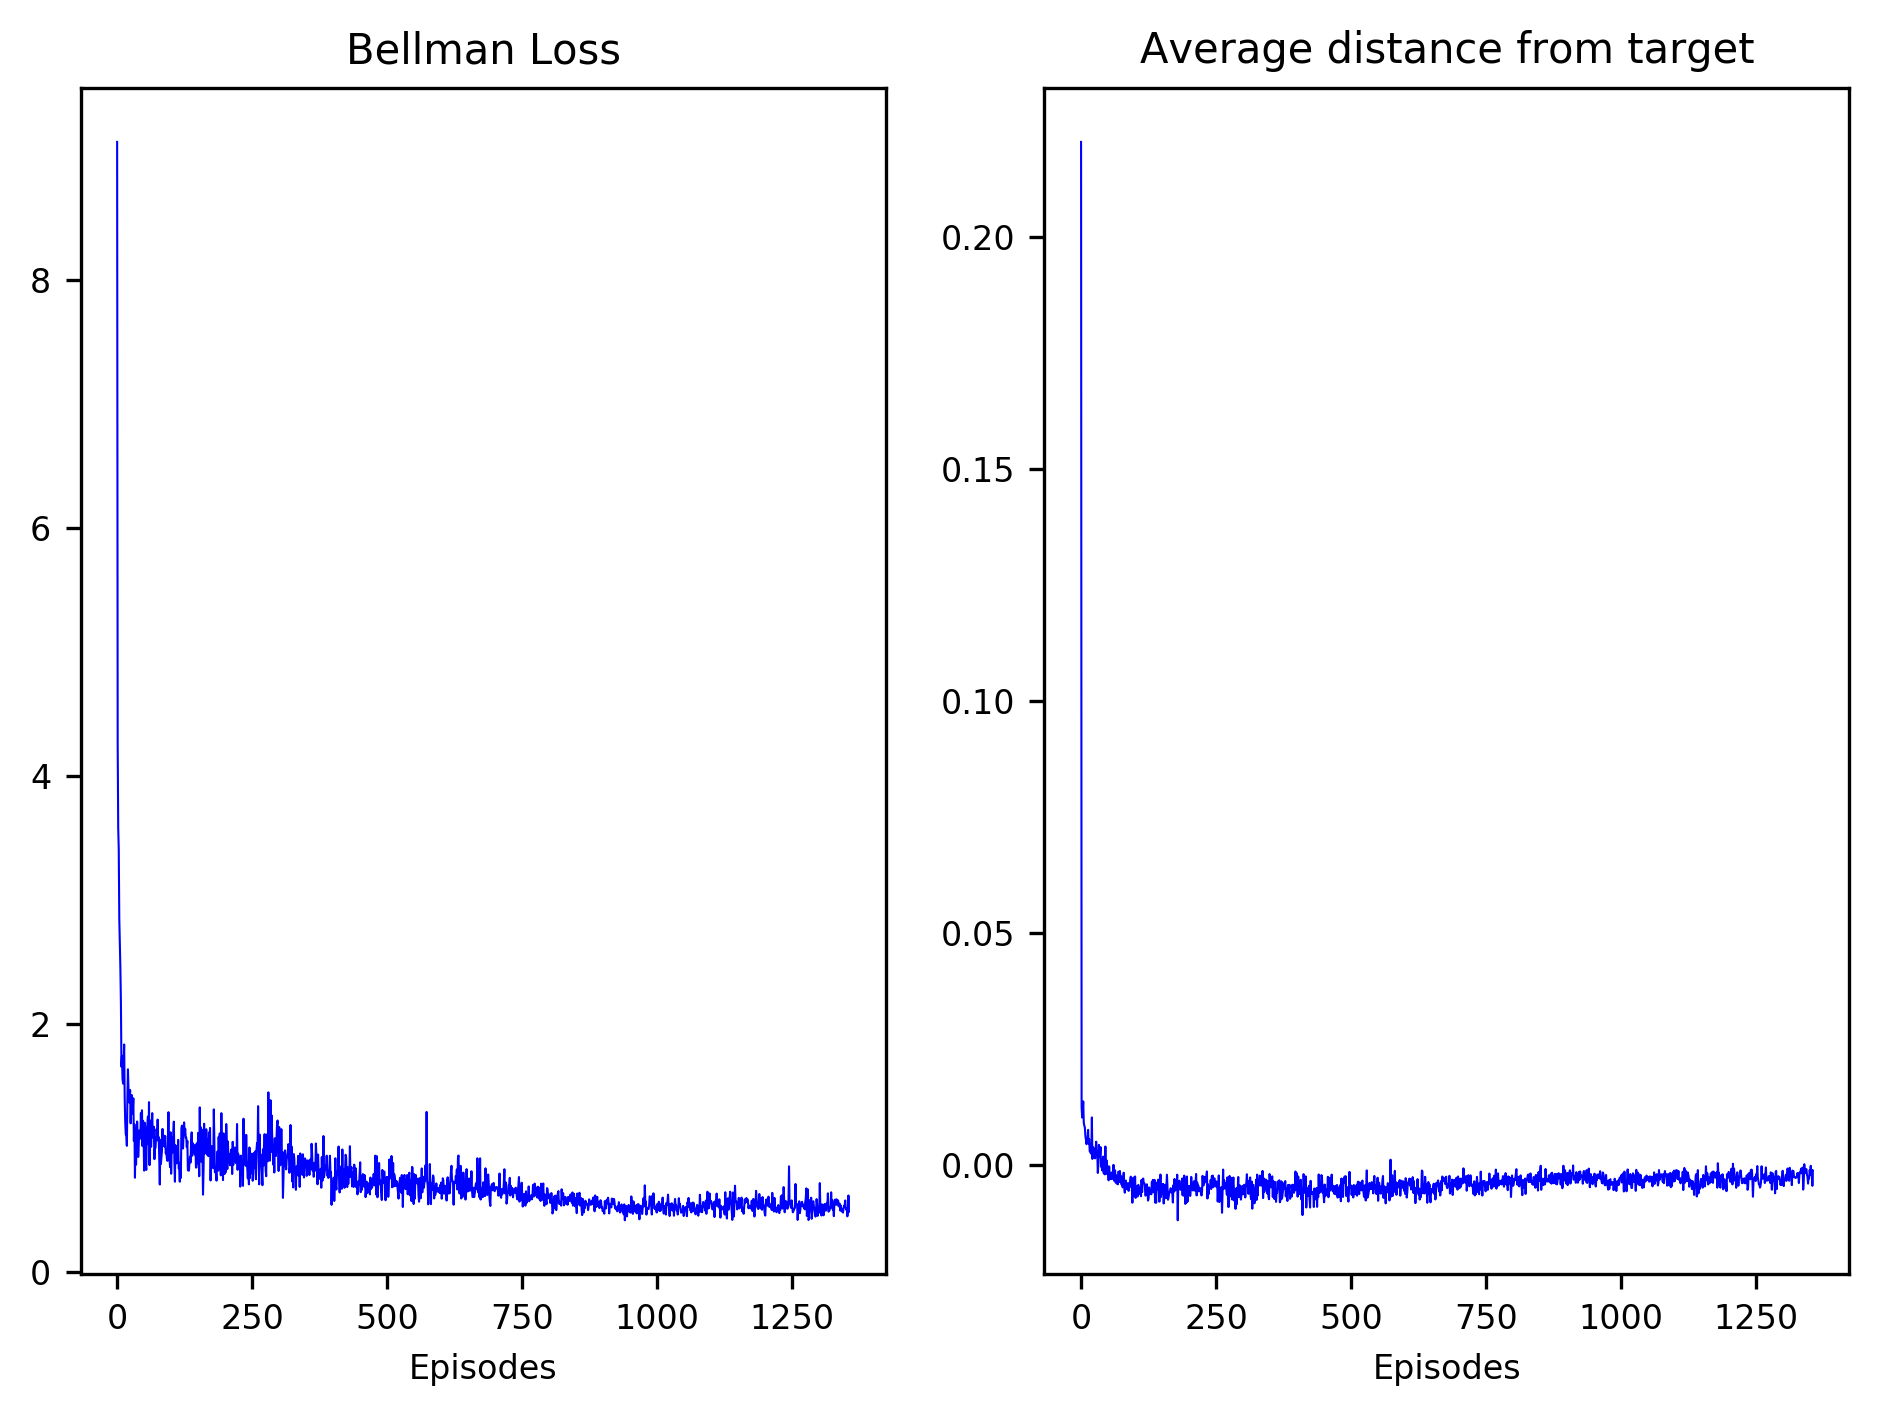
\includegraphics[height=10cm]{{figures/b34_1_0.00001_500000_train}.png}
	\end{center}
\end{figure}

This curve closely resembles a supervised learning curve. The loss does not strictly reduce from one step to the next, for perhaps a few reasons: 1) When using neural networks, this behaviour is not guaranteed, and 2) the loss is being calculated against some sample of the experience, which might have never been seen before, and hence cause the algorithm to predict incorrectly and result in a high loss.

\subsubsection{Boxing}
After hyperparameter optimisation using grid-search, the best performing agent was selected. The image was downsampled to $40 \times 40 \times 1$; the learning rate chosen was 0.0001; $\epsilon$ was set to 0.1 throughout training. The agent was trained for 1,000,000 steps.

\begin{figure}[H]
    \caption{%
		Bellman loss and distance from target for agent while learing to play Boxing
     }%
	\begin{center}
     	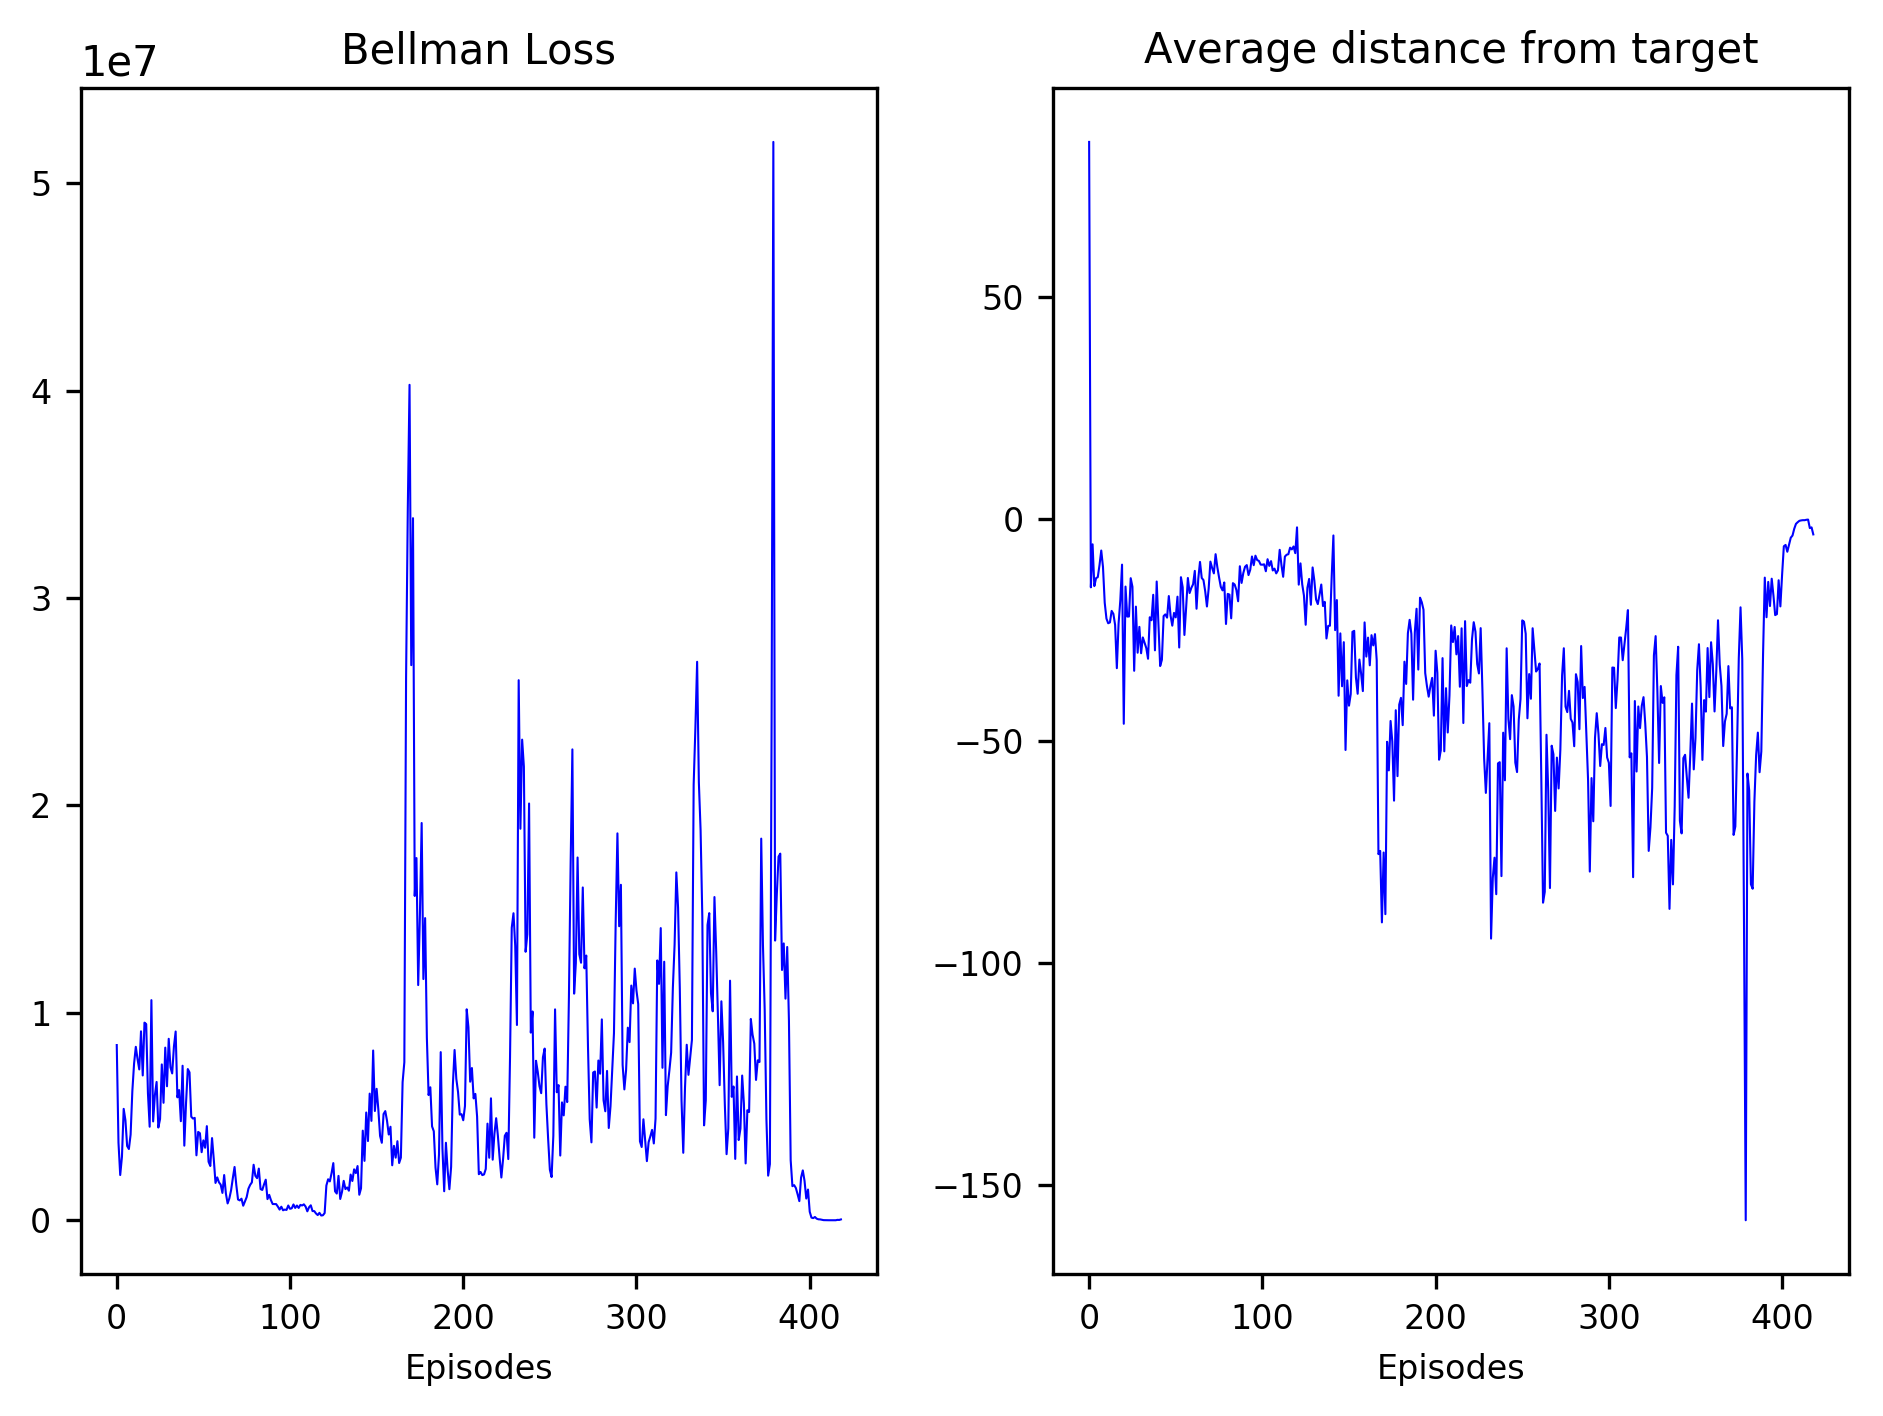
\includegraphics[height=10cm]{{figures/b34_2_0.0001_0_train}.png}
	\end{center}
\end{figure}

This graph is significantly different from other graphs. It might be that the learning rate was too high for this particular experiment.\\

Finally, reinforcement learning loss curves can be different from supervised learning loss curves because the algorithms are fundamentally updating towards different values. Supervised learning algorithms update toward the 'true' or 'gold' value, while most reinforcement learning algorithms (ones that do not sample to the of an episode) are updating toward some \textit{approximation} of the final result. This approximation may be biased in some way: for example, Q-learning overestimates the q-values of a Markov Decision Process. If the approximation is poor (due to the current initialisations, or the current target values, or poor recent experience) it can be source of noise causing the loss curve to look strange.

\subsection{Testing the Atari agents}

Presented below are graphs of Average moves and Discounted Reward over multiple evaluation trials, plotted every 50,000 steps during training. 

\subsubsection{Pong}
We can see the average length of the episode during evalution increases with more training. Also, the discounted rewards trend upward, in spite of having high variance. Our final Pong agent achieves an average discounted reward of -0.4422 over a hundred trials.

\begin{figure}[H]
    \caption{%
		Average episode length and discounted rewards at evaluations every 50,000 steps while learning Pong.
     }%
	\begin{center}
     	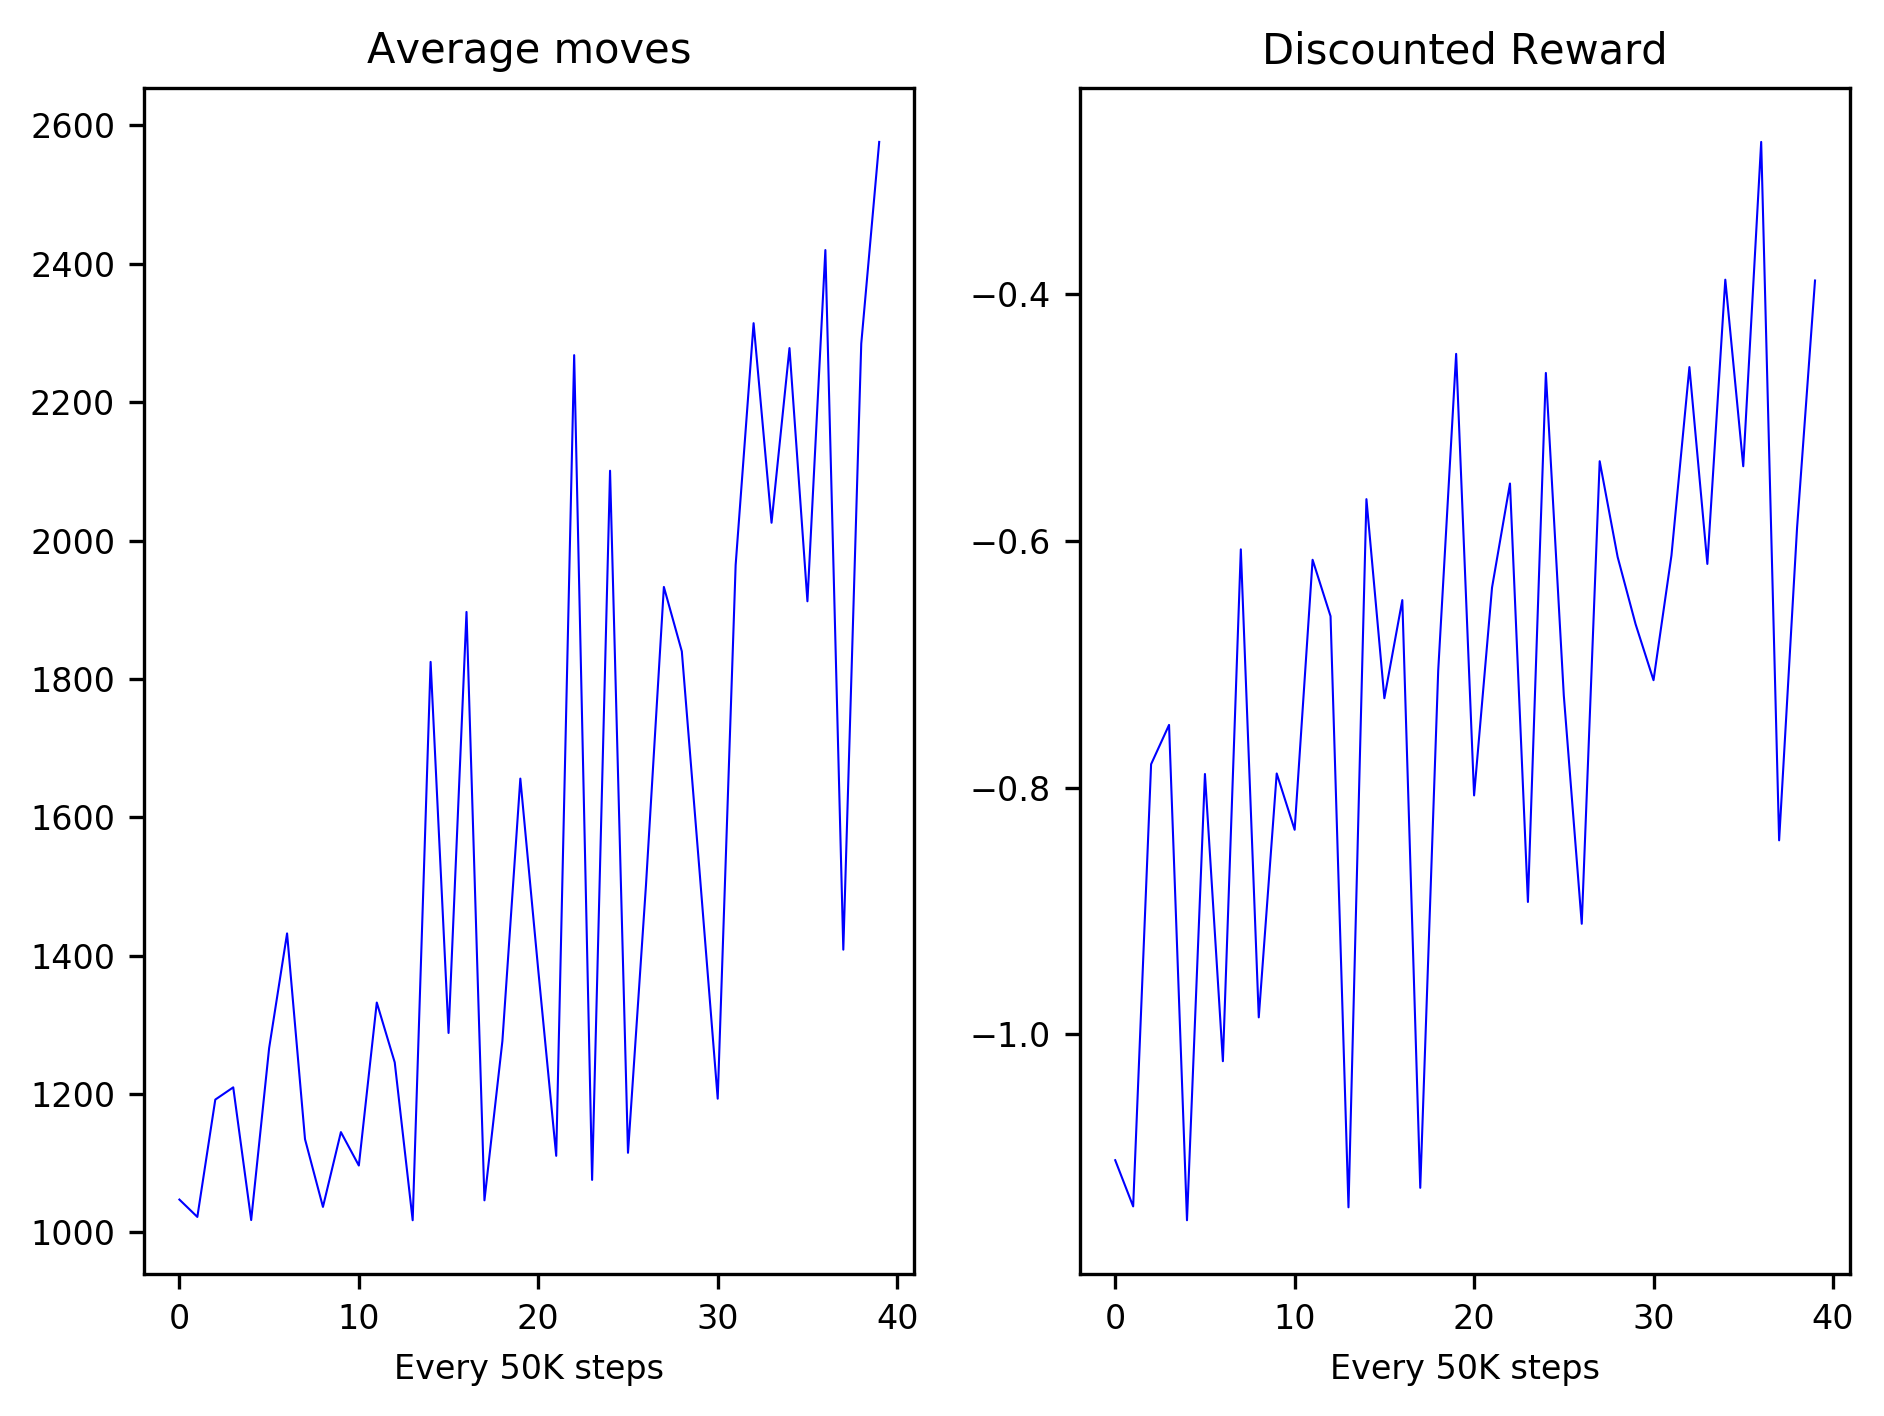
\includegraphics[height=10cm]{{figures/b34_0_0.00001_0_test}.png}
	\end{center}
\end{figure}

The Pong agent attempts to hit the ball almost every time. It often manages to score two to four points against the opponent.

\subsubsection{Ms Pacman}
Again, we can see the average length of the episode during evalution increases with more training. Also, the discounted rewards trend upward, in spite of having high variance; however, this is lower than that for Pong. Our final Ms Pacman agent achieves an average discounted reward of 5.0694 over a hundred trials.

\begin{figure}[H]
    \caption{%
		Average episode length and discounted rewards at evaluations every 50,000 steps while learning Ms Pacman.
     }%
	\begin{center}
     	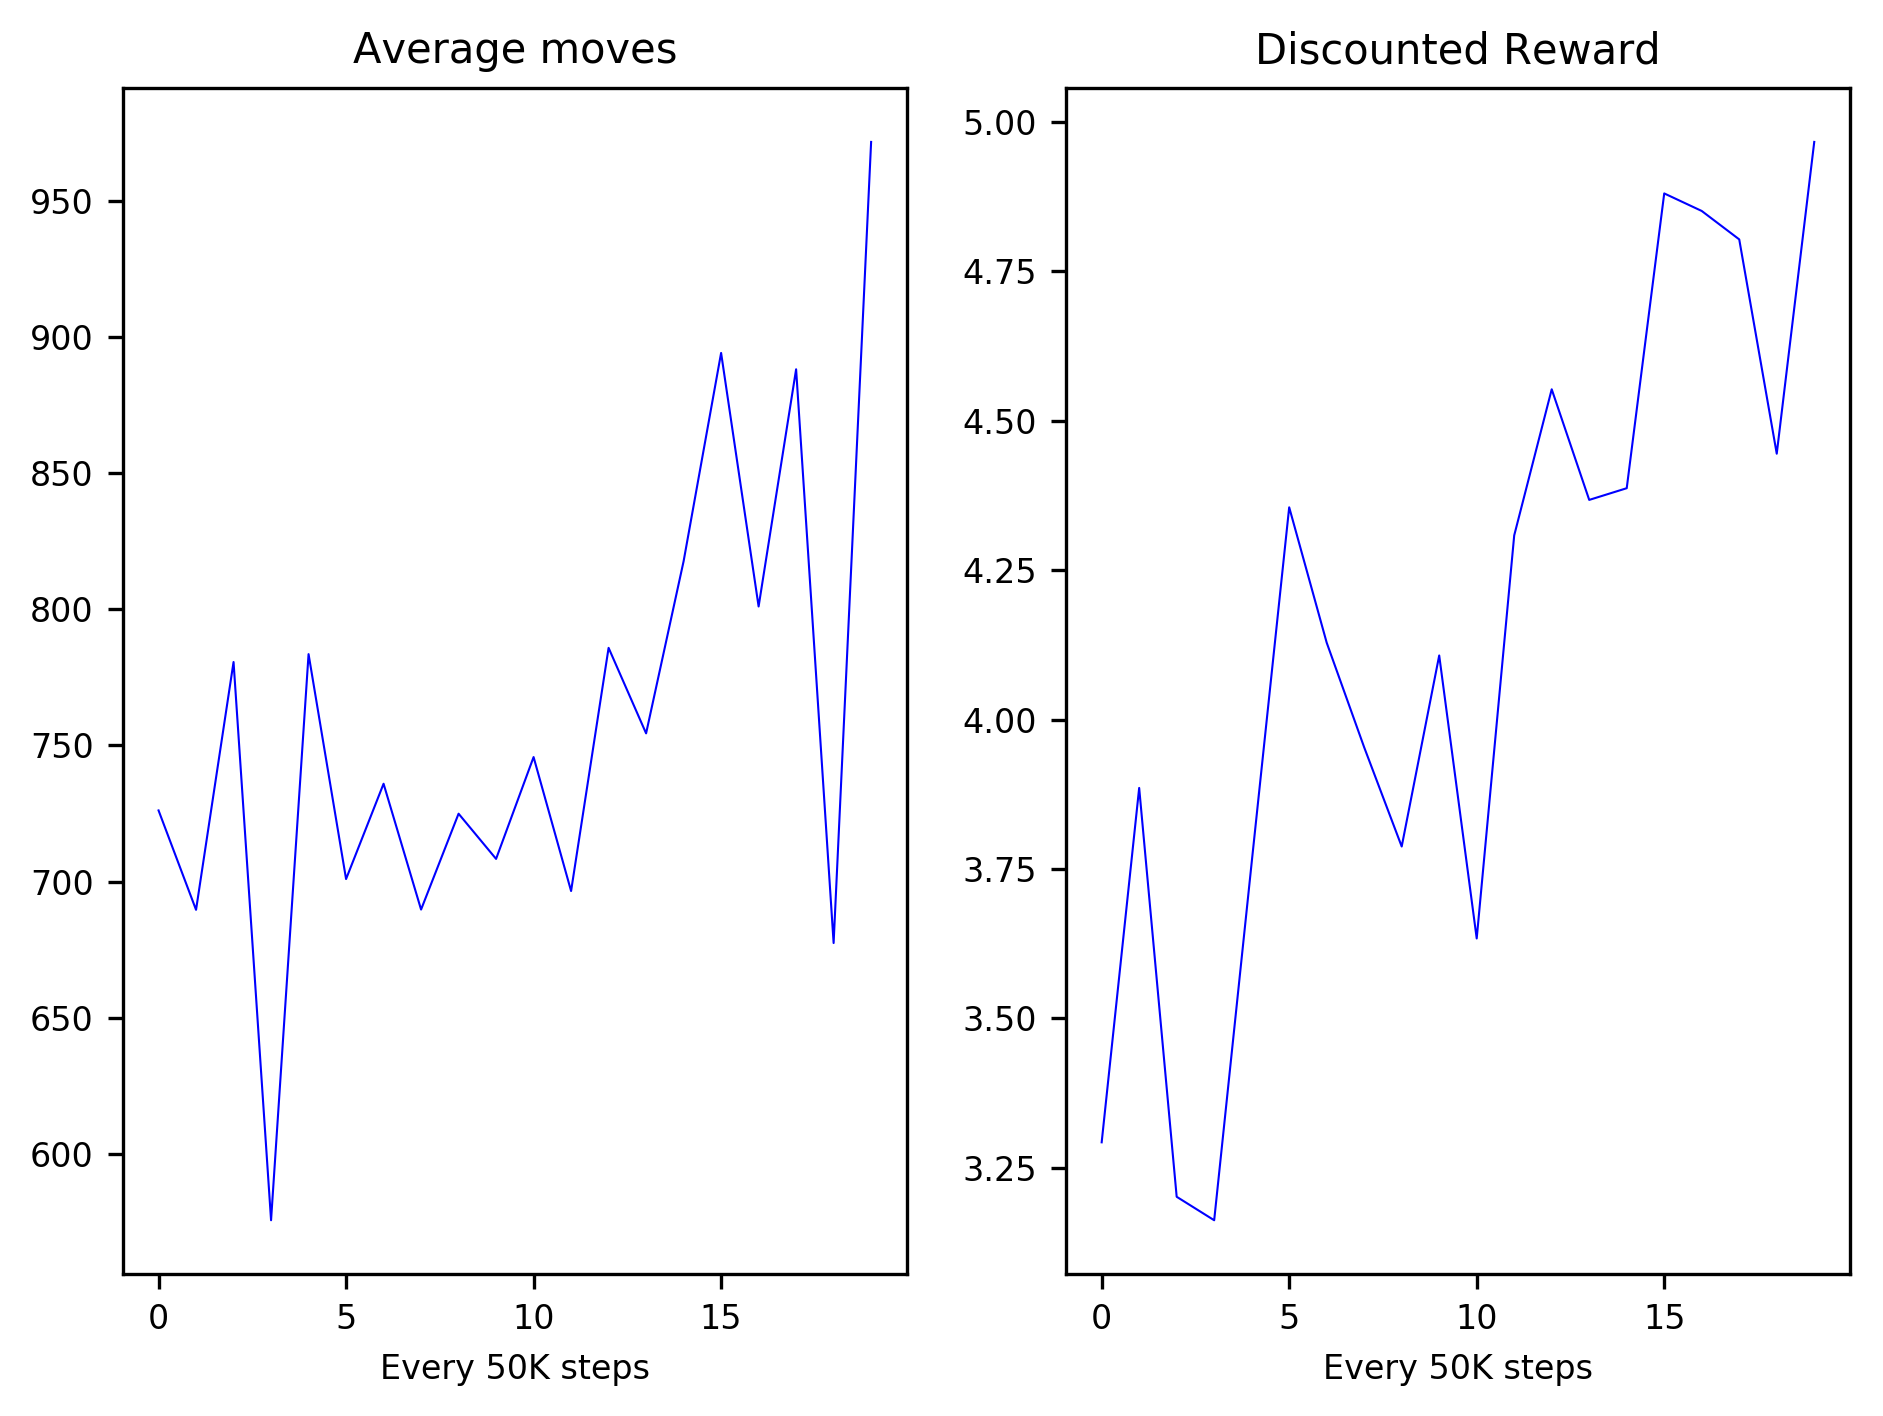
\includegraphics[height=10cm]{{figures/b34_1_0.00001_500000_test}.png}
	\end{center}
\end{figure}

The Ms Pacman agent runs around the maze in different patterns each time. It rarely if ever stops moving; however, it does not seem to be interested in eating pellets all the time.

\subsubsection{Boxing}
The length of an episode is fixed in this game. Also, the discounted reward does not seem to follow a learning trend; however, among all the agents, this one was the only one able to consistently perform better than random. Our final Boxing agent achieves an average discounted reward of 0.7436 over a hundred trials.

\begin{figure}[H]
    \caption{%
		Average episode length and discounted rewards at evaluations every 50,000 steps while learning Boxing.
     }%
	\begin{center}
     	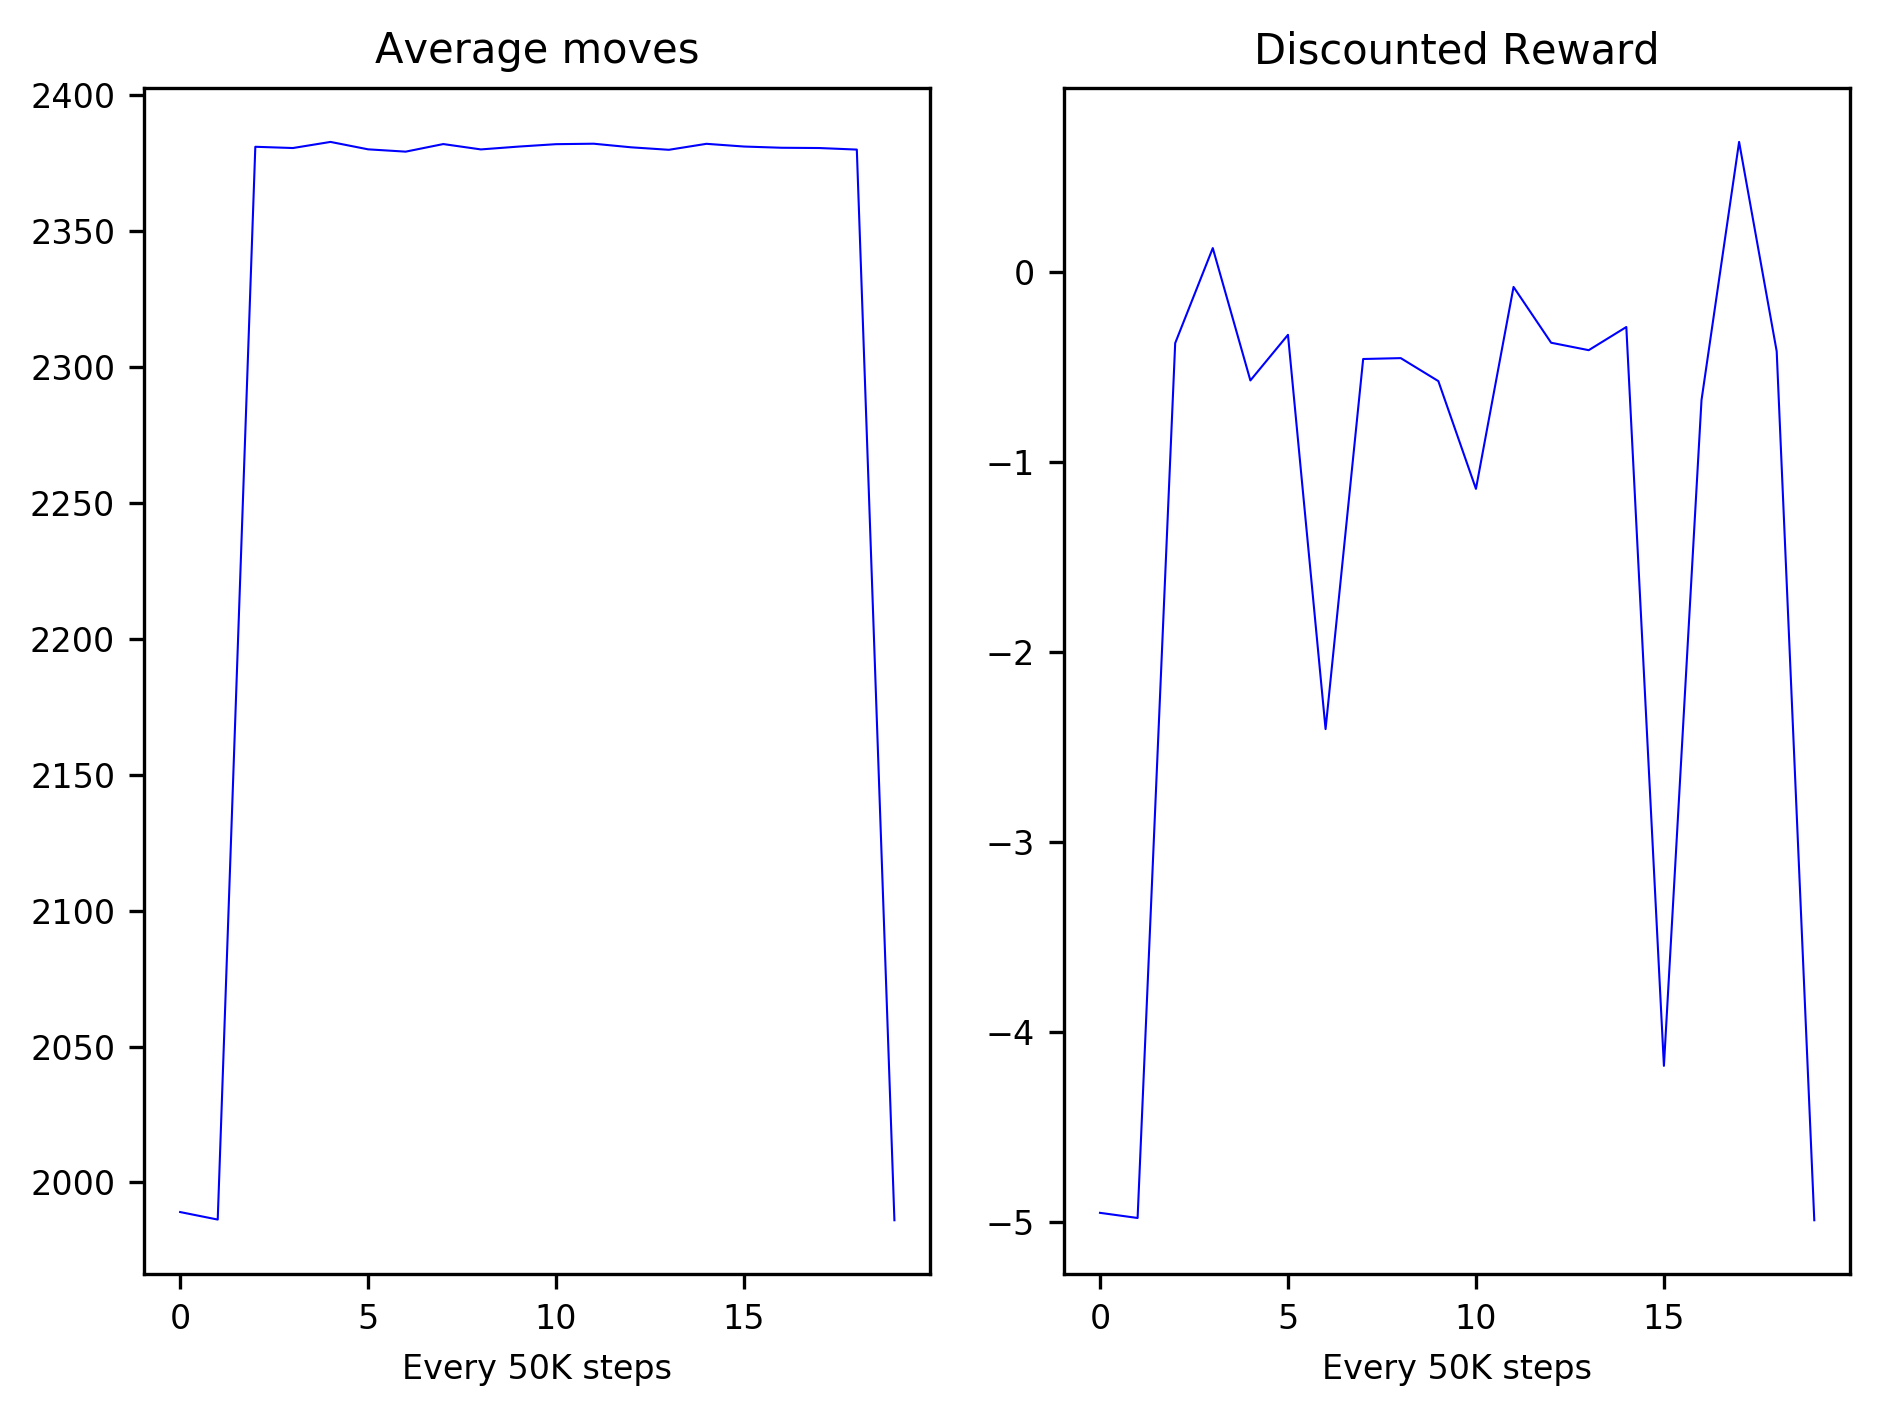
\includegraphics[height=10cm]{{figures/b34_2_0.0001_0_test}.png}
	\end{center}
\end{figure}

The boxing agent usually gets a couple of quick hits early on in the game, allowing it to secure a discounted reward which is positive. It still loses the game almost every time, but sometimes by very close margins. It also blocks the other boxer from making too many hits for the duration of the game.



%----------------------------------------------------------------------------------------

\end{document}